\documentclass[12pt,a4paper,english]{article} 
\batchmode

\voffset -1.0cm
\textheight 23cm
\hoffset -1.2cm
\textwidth 15.6cm

%%\usepackage[T1]{fontenc}
\usepackage[latin1]{inputenc} 
\usepackage{babel} 
\usepackage{setspace}
\usepackage{gromosXX}

%% \usepackage{fancyheadings}
\usepackage{pslatex}
\usepackage{epsfig}
\usepackage{graphicx}
\usepackage{units}
\usepackage{booktabs}

%%\usepackage{cite}
\usepackage{citesort}  
\usepackage{overcite}
%%\usepackage{latexsym}

\usepackage{amsmath}
\usepackage{amsfonts}

\usepackage{listings}

%%\doublespacing

\newcommand{\mbf}[1]{\mathbf{#1}}
\newcommand{\deri}[2]{\frac{\partial #2}{\partial #1}}
\renewcommand{\baselinestretch}{1.5}
\newcommand{\noun}[1]{\textsc{#1}}
\renewcommand{\thetable}{\Roman{table}}

\begin{document}

\title{The \noun{Gromos} software for biomolecular simulation: \noun{Gromos05}}
\date{\today}
\author{Markus Christen, Philippe H. H\"unenberger, Dirk Bakowies, Riccardo
  Baron, \\ Roland B\"urgi$^a$,
  Daan P. Geerke, Tim N. Heinz, Mika A. Kastenholz,
  Vincent Kr\"autler, \\
  Chris Oostenbrink$^b$, Christine Peter$^c$, Daniel
  Trzesniak,\\
  and Wilfred F. van Gunsteren
  \thanks{Corresponding author (wfvgn@igc.phys.chem.ethz.ch)}
}

\lstset{language=C++}

\maketitle
\noindent
    {Laboratory of Physical Chemistry, Swiss Federal Institute of
      Technology Z\"urich, ETH-H\"onggerberg, CH-8093 Z\"urich,
      Switzerland} \\
    Present addresses: \\
    $^a${Swissre, Z\"urich, Switzerland} \\
    $^b${Vrije Universiteit, Pharmaceutical Sciences / Pharmacochemistry, De
      Boelelaan 1083 P262, NL-1081 HV Amsterdam, The Netherlands} \\
    $^c${Max-Planck-Institute for Polymer Research, Ackermannweg 10, D-55128 Mainz, Germany} \\

\newpage

\begin{abstract}
We present the latest version of the Groningen Molecular Simulation
program package, \noun{Gromos05}. It has been developed for the dynamical
modelling of (bio)molecules using the methods of molecular dynamics,
stochastic dynamics, and energy minimisation. An overview of \noun{Gromos05} is
given, highlighting features not present in the last major release,
\noun{Gromos96}. The organisation of the program package is outlined and the
included analysis package \noun{Gromos++} is described. Finally, some
applications illustrating the various available functionalities are presented.
\newline
{\textbf{Keywords:} molecular dynamics simulation, programming, \noun{Gromos},
  biomolecular simulation
}
\end{abstract}

\newpage

\section{Introduction}
Starting with \noun{Gromos80}, the \noun{Gromos} program package has
been developed over the past 25 years to facilitate research efforts
in the field of biomolecular simulation in a university environment. The
\noun{Gromos} software was and is
meant for use in a scientific environment, which may be characterised by
a continuously changing flow of users, who either wish to investigate
and implement new simulation algorithms or intend to carry out
applications of simulation in a variety of fields, ranging from
polymers, glasses
and liquid crystals to crystals and solutions of biomolecules (proteins,
nucleic acids, saccharides and lipids). To this purpose
\noun{Gromos} has been developed based on the following principles:
({\em i}) transparency
of the code, making modifications easy, 
({\em ii}) modular architecture, so
that only parts of it need be modified for the implementation of new
functionalities designed
by users, 
({\em iii}) independence of the
simulation code and the force field, and
({\em iv}) independence of the
simulation code and the
computer hardware. The major releases of the \noun{Gromos}
software are \noun{Gromos87} \cite{G87,MD95.33} developed at the University of
Groningen, \noun{Gromos96}\cite{MD96.40, MD99.11} developed at ETH Z\"urich, and now \noun{Gromos05}.
\noun{Gromos} has found widespread use (hundreds of licences in over 57 countries on all
continents except Antarctica, see \reffig{gromosworld}), triggered by the fact that it
has been designed for ease of 
extendability and that the complete source code is made available to
research establishments for a nominal fee \cite{homepage}. The program code has been
further developed in the group for computational chemistry at ETH
Z\"urich (Switzerland) throughout the recent years, leading now to a new
major release, \noun{Gromos05}. The enhancements were governed by the following
criteria: (1) interest of our research group \cite{MD01.34}, (2) ease of use, (3)
extendability, (4) demonstrated usefulness or efficiency of new methods, (5)
well-defined and correct formulae and algorithms, and (6) computational
efficiency. The second criterium led to a complete rewrite of the
setup and analysis tools, now contained in the \noun{Gromos++} setup and
analysis subpackage, written
in \noun{C++}. The third criterium led to a rewrite in \noun{C++} of the MD
engine,
the part that carries out molecular dynamics (MD) or stochastic dynamics (SD)
simulations as well as energy minimisations (EM), into a new program
called MD++.
In parallel, the original \noun{Fortran} version of the MD engine,
PROMD, was further developed to introduce many new features (some of
which are not yet available in MD++). On the long term (beyond
\noun{Gromos05}), MD++ will entirely replace PROMD.

In the next sections the main features of \noun{Gromos05} are described. In
section 2 new functionalities with respect to \noun{Gromos96} are
highlighted and in section 3 follows the algorithmic description of
selected new functionalities.
In section 4, the organisation of the
code is discussed and an overview of the programs present
in the \noun{Gromos++} analysis subpackage is provided. In section 5, examples of
applications are reported for some of the newer features. Section 6 provides a
summary and conclusions.

\section{Overview of functionalities}

Here, the main features of the two MD engines available in
\noun{Gromos05}, PROMD and MD++ are described.
These two programs share most of the basic functionalities, but still
differ in a number of aspects.The FORTRAN MD engine (PROMD) retains all
features of the \noun{Gromos96} release and adds a number of new
functionalities. The \noun{C++} MD engine (MD++) contains most of the \noun{Gromos96} features
(except four-dimensional and path integral simulations), a subset of the new
functionalities recently introduced into PROMD (since the
\noun{Gromos96} release), and some new features of its own.

A non exhaustive list of the features included is:
\begin{itemize}
\item Molecular dynamics (MD), stochastic dynamics (SD) simulation and
  energy minimisation (EM; steepest descent or conjugate gradient);
\item Periodic boundary conditions (vacuum, rectangular, truncated
  octahedral or triclinic computational box; possibility of performing
  multiple-unit-cell simulations);
\item Temperature control (constraining, weak coupling,
  Nos\'{e}-Hoover or Nos\'{e}-Hoover
  chain; possible coupling of different subsets of degrees of freedom to
  separate temperature baths);
\item Pressure control (weak coupling or Andersen-Parrinello-Rahman:
  isotropic, partially anisotropic
  and fully anisotropic coordinate scaling; atom-based or group-based
  pressure definition);
\item Long-range electrostatic interactions: straight cutoff truncation,
  truncation with Poisson-Boltzmann reaction field (RF) correction and lattice-sum (LS)
  methods, including Ewald summation,
  particle-particle-particle-mesh (P$^3$M);
\item Charge-group based or atom-based cutoff for the non-bonded interactions;
\item Grid based pairlist construction;
\item Non-physical interactions: atom-position, atom-distance, dihedral-angle, NOE and J-value
  restraints as well as atom-position and atom-distance constraints (SHAKE, M-SHAKE, LINCS);
\item Enhanced sampling: local elevation MD, replica exchange MD
  (REMD) and umbrella sampling;
\item Calculation of free energy changes based on the coupling parameter
  ($\lambda$) approach using thermodynamic integration, slow-growth
  or one-step perturbation, possibly including soft-core
  nonbonded interactions;
\item Path integral simulation;
\item MPI and OMP parallelisation;
\end{itemize}

A number of the new features introduced in \noun{Gromos05} are discussed
in section 3.2. Pre-exisiting features have been described in details
elsewhere \cite{MD96.40, MD99.11}. The functionalities of the
pre- and post-processing programs contained
in \noun{Gromos++} are discussed in section 4.3.
A complete description of the available features will be included in the
new \noun{Gromos} manuals.

\section{Algorithms}

\subsection{MD algorithm}

The complete MD algorithm based on the leap-frog scheme as implemented
in \noun{Gromos} is the following \cite{MD96.40}. Given initial atomic positions and
velocities, which satisfy any given geometrical constraints:

\begin{enumerate}
\item Save positions (reset atomic coordinates into the reference computational box
  in case of periodic boundary conditions) and velocities for later analysis.
\item Remove centre of mass motion (if required).
\item Calculate (unconstrained) energies, forces and virial contribution from the potential energy
  function (using the nearest image convention in case of periodic boundary
  conditions). Save these.
\item Enforce any given position constraints by resetting the forces and velocities of
  positionally constrained atoms to zero.
\item Update the velocities using the leap-frog scheme.
\item Apply temperature coupling (constraining, weak coupling,
  Nos\'{e}-Hoover or Nos\'{e}-Hoover chain) by scaling the atom velocities.
\item Update the positions using the leap-frog scheme.
\item Enforce distance constraints (using SHAKE, M-SHAKE or LINCS) both
  for positions and velocities, and calculate the corresponding forces
  and virial contribution. Save these.
\item Calculate the kinetic energy and temperature (possibly on the
  basis of separate subsets of degrees of freedom).
\item Calculate the pressure (atom-based or group-based pressure definition).
\item Apply pressure scaling (weak coupling or Parrinello-Rahman) by
  scaling atomic positions (isotropic, partially anisotropic or
  fully anisotropic scaling).
\item Update the coupling parameter $\lambda$ for (free
  energy) simulations involving $\lambda$ changes (slow growth).
\item Calculate total energies, averages and fluctuations. Save these.
\end{enumerate}

This sequence is repeated for the required number of simulation steps.

\subsection{New features}

\subsubsection{Spatial boundary conditions}

\label{spatial_boundary_cond}
Spatial boundary conditions are defined by 
the shape, size and orientation of the simulated system, 
and the nature of the boundary to its surroundings.
%
The GROMOS05 implementation (both PROMD and MD++)
admits four types of boundary conditions:
($i$) vacuum boundary conditions;
($ii$) periodic boundary conditions based on a rectangular box; 
($iii$) periodic boundary conditions based on a truncated-octahedral box;
($iv$) periodic boundary conditions based on a triclinic box.
%
In the three latter cases, 
the system is confined to a (reference) computational 
box that is surrounded by an infinite number of periodic 
copies of itself.
%


When periodic boundary conditions are applied, 
the shape, size and orientation
of the computational box must be defined.
%
For rectangular and triclinic periodic boundary conditions, 
this is done by specifying the three edge vectors
$\av$, $\bv$ and $\cv$ (defining a right-handed coordinate 
system) of the reference computational 
box. For a truncated-octahedral box, these 
vectors correspond instead to the edges of the cube based on which the 
truncated octahedron is constructed.
%
In practice,
the three vectors are specified by their lengths $a$, $b$ and $c$,
the box angles $\alpha$ (between $\av$ and $\bv$), $\beta$
(between $\av$ and $\cv$) and $\gamma$ (between $\bv$ and $\cv$)
they define among each other
(all in the range $]0;\pi[$), 
and the three 
Euler rotation angles $\phi$, $\theta$ and $\psi$ 
(the two former ones in the range $]-\pi;\pi]$,
the latter one in the range $[-\pi/2;\pi/2]$)
characterising the orientation of the box relative 
to the reference right-handed Cartesian coordinate system 
$(\ev_{x},\ev_{y},\ev_{z})$.
%
To define the Euler angles, 
the three edge vectors are used to define 
a box-linked right-handed Cartesian coordinate system 
$(\ev_{x'},\ev_{y'},\ev_{z'})$ in the following way:
($i$) the $x'$-axis is chosen along and in the direction of $\av$;
($ii$) the $y'$-axis is chosen orthogonal to $\av$ in the plane 
       defined by $\av$ and $\bv$, and oriented in the direction 
       of $\bv$;
($iii$) the $z'$-axis is chosen orthogonal to both $\av$ and $\bv$,
       and oriented in the direction of $\cv$.
%
%
The reference coordinate system can be rotated onto the 
box-linked coordinate system by the following series
of rotations:
%
($i$) a rotation by an angle $\phi$ around the $z$-axis;
($ii$) a rotation by an angle $\theta$ around the new $y$-axis;
($iii$) a rotation by an angle $\psi$ around the new $x$-axis.
%
The angles $\phi$, $\theta$ and $\psi$ thus represent the three 
Euler rotation angles in a $zyx$ or yaw-pitch-roll convention.
%(by analogy with an airplane flying along the 
%$x'$-axis and with its wings along the $y'$-axis,
%where $\phi$, $\theta$ and $\psi$ represent the 
%yaw, pitch and roll of the airplane).
%
The use of a rectangular or truncated-octahedral box 
requires $\alpha=\beta=\gamma=\pi/2$
and is restricted to non-rotated boxes with
$\phi=\theta=\psi=0$.
%
The use of a truncated-octahedral box also 
requires $a=b=c$.
%
In the case of vacuum boundary conditions, the system 
is non-periodic, and $\av$, $\bv$ and $\cv$
need not be specified.



Based on a general triclinic box in an arbitrary orientation,
the position of an atom may be specified 
through coordinates $\rv=(x,y,z)$ 
within the reference Cartesian coordinate system
$(\ev_{x},\ev_{y},\ev_{z})$,
or through oblique fractional coordinates $\tauv=(u,v,w)$
with reference to the box-edge vectors.
%
The two types of coordinates are related by
%
\beq{frac_to_obli}
   \rv = \Lmtr\tauv \ , 
\eeq
%
where the matrix $\Lmtr$ 
contains the components of $\av$, $\bv$ and $\cv$ 
in the reference Cartesian coordinate system
as its columns.
%
The box volume is
\beq{box_volume}
   V = |\Lmtr| \ .
\eeq
%
This matrix can be decomposed as 
%
\beq{lmtr_matrix}
  \Lmtr = 
   \left(\begin{array}{ccc}
    a_x & b_x & c_x \\
    a_y & b_y & c_y \\
    a_z & b_z & c_z 
  \end{array}\right) 
= \Rmtr\,\Smtr
\ ,
\eeq
%
where the orthogonal transformation matrix $\Rmtr$
(rotation between reference and box-linked 
Cartesian coordinate systems) is given by
%
\beq{spacial_transfo_box_linked_to_ref_matrix}
  \Rmtr =
   \left(\begin{array}{ccc}
    \cos\theta\cos\phi & 
    \sin\psi\sin\theta\cos\phi-\cos\psi\sin\phi & 
    \cos\psi\sin\theta\cos\phi+\sin\psi\sin\phi \\
    \cos\theta\sin\phi & 
    \sin\psi\sin\theta\sin\phi+\cos\psi\cos\phi &
    \cos\psi\sin\theta\sin\phi-\sin\psi\cos\phi \\
    -\sin\theta &
    \sin\psi\cos\theta &
    \cos\psi\cos\theta
  \end{array}\right) \ ,
\eeq
%
and the transformation matrix $\Smtr$
(between box-linked Cartesian coordinates and 
oblique fractional coordinates) is given by
%
\beq{spacial_transfo_obl_to_box_linked_matrix}
  \Smtr = 
   \left(\begin{array}{ccc}
    a & b\cos\gamma & c\cos\beta \\
    0 & b\sin\gamma & c\sin\beta\cos\delta \\
    0 & 0 & c\sin\beta\sin\delta
  \end{array}\right) \ ,
\eeq
%
with
%
\beq{spacial_tric_delta_def}
  \cos\delta = \frac{\cos\alpha - \cos\beta\cos\gamma}
                    {\sin\beta\sin\gamma}
  \ \ \ , \ \ \ 
   \delta\in ]0;\pi[ \ .
\eeq
%


As shown by Bekker \cite{BE97.2}, a simulation 
performed in a truncated-octahedral box
can equivalently be performed in a special type of triclinic
box, by applying an appropriate coordinate transformation.
%
%If the edge vectors of the cube based on which the 
%truncated-octahedron is constructed are $\av$, $\bv$ and 
%$\cv$ (recall that $a=b=c$, $\alpha=\beta=\gamma=\pi/2$
%and  $\phi=\theta=\psi=0$ in this case), 
%
A possible choice for 
the edges $\av_t$, $\bv_t$ and 
$\cv_t$ of the transformed triclinic box is
%
\beq{spacial_octa_tric}
  \av_t = \av \ \ \ ,\ \ \ 
  \bv_t = (1/2) (\av+\bv+\cv) \ \ \ \mathrm{and}\ \ \ 
  \cv_t = (1/2) (-\av-\bv+\cv) \ .
\eeq
%
The corresponding box-edge lengths, box angles and Euler angles
are
$a_t=a$,
$b_t=c_t=(\sqrt{3}/2)a$,
$\alpha_t=\mathrm{acos}(-1/3)\approx 109.5^o$,
$\beta_t=\mathrm{acos}(-1/\sqrt{3})\approx 125.3^o$,
$\gamma_t=\mathrm{acos}(1/\sqrt{3})\approx 54.8^o$,
$\phi_t=\theta_t=0$, and 
$\psi_t=45^o$.
%
The mapping of atomic coordinates within a truncated-octahedral 
box to atomic coordinates within the transformed triclinic box
is performed by applying shifts along the 
$\av_t$, $\bv_t$ and $\cv_t$ vectors.
%
This formalism is applied for the gereralisation of 
grid-based pairlist algorithms (section 3.2.7)
and lattice-sum electrostatics (section 3.2.9) 
to truncated-octahedral boxes.
%
Because the truncated-octahedral case can always be 
mapped to the triclinic case, 
subsequent sections will only discuss the case of the triclinic box.
%
% MD++ conceded to reality and implements all boundary conditions
%

%In a general triclinic box, 
%the square length of a vector is given in terms 
%of the corresponding oblique coordinates 
%by 
%%
%\beq{tric_square_len}
%  r^2 =  u^2+v^2+w^2 
%        +2uv\cos\gamma + 2uw\cos\beta 
%     + 2vw \cos\alpha
%\ .  
%\eeq
%
%The volume of a triclinic box is given by
%%
%\beq{tric_volume}
%  V =  abc [ 1-\cos^2\alpha-\cos^2\beta-\cos^2\gamma
%            +2\cos\alpha\cos\beta\cos\gamma]^{1/2} \ ,
%\eeq
%%
%while the volume of a truncated-octahedron box 
%is given by
%%
%\beq{truncoct_volume}
%  V = (1/2) a^3 \ .
%\eeq
%%
%The volume of the triclinic box equivalent to 
%a truncated-octahedral 
%box (\refsec{spacial_bound_cond_ctransf_truncoct}) 
%is identical to that of the original box.
%



%It may be necessary to tranform rank-two tensors 
%(3$\times$3 matrices) among the various coordinate 
%representations.
%
%If a tensor is written $\Omegamtr$ in terms 
%of oblique fractional coordinates
%and $\Wmtr$ in the reference Cartesian coordinate system, 
%the conversion between the different representations
%is given by%
%
%
%
%\beq{spacial_tensor_transfo_1}
%  \Wmtr = \Lmtr \, \Omegamtr\,{}^t\Lmtr \ .
%\eeq
%
%In practice, this transformations are used to interconvert
%the various representations of the virial tensor (section XXX).


\subsubsection{Multiple-unit-cell simulations}

Within the GROMOS05 implementation (both PROMD and MD++), 
it is possible to simulate a periodic 
computational box (rectangular or triclinic only)
consisting of multiple periodic copies 
of a smaller unit cell (referred to here as subcells).
%
This option may be useful when trying to simulate 
a single unit cell of a crystal that is too small to allow 
for the application of a reasonably large cutoff value.
%
The number of subcell boundaries
along the three box-edge vectors $\av$, $\bv$ and $\cv$ 
are $M_a$, $M_b$ and $M_c$, so that the total 
number of subcells is $M=M_a\cdot M_b\cdot M_c$.
%
In this case, the total number of solute molecules 
and the total number of solvent molecules must 
both be integer multiples of $M$.
%

Subcell periodicity within the computational box must 
be fulfilled by the initial coordinates and velocities, 
and will then be maintained throughout the simulation.
%
%The solute and solvent molecules must be grouped by subcells
%(always in the same order), and follow a sequence 
%defined by successive subcells in a line (increasing $m_a$), 
%in a row (increasing $m_b$) and in a plane (increasing $m_c$), 
%taking periodicity into account,
%where $m_a$, $m_b$ and $m_c$ are integers defining the 
%location of the different subcells within the computational box.
%
%More precisely, solute atom number $i$ of the 
%first solute molecule is related 
%by periodicity to its $M$ copies with atom numbers 
%$j=i+(M_aM_bm_c+M_am_b+m_c)\mathrm{NRP}$,
%
%This means that atom $i$ shares identical forces and velocities
%with the $M$ atoms $j$, and that their connecting vector 
%(in units of the lattice defined by the subcells) is the minimum 
%image of $\mv$.
%
%A similar relationship holds for solvent atoms.
%
%
The corresponding periodicity constraints on the forces, 
velocities and coordinates are checked at each step of the 
simulation, with reference to the 
subset of solute and 
solvent molecules with the smallest sequence numbers.
%
%The periodicity constraints on the forces, velocities and 
%coordinates are checked at the beginning of each step.
%
Deviations smaller than user-specified tolerances
(numerical drift) are systematically corrected. 
Deviations larger than the tolerance are reported as an
error.
%XXX
%Any deviation larger than $\Delta_v$ (in absolute value) 
%results in an error message, while any smaller deviation is 
%corrected without warning.
%XXX


Note that the removal of the center of mass motion
(section~3.2.3), whenever 
required, is applied to charge groups and solvent molecules 
gathered
in the individual subcells.
%
Note also that the application of the particle-particle-particle-mesh (P$^3$M) method
to evaluate electrostatic interactions
(section~3.2.9) will only give rise to exactly periodic forces if 
the number of P$^3$M grid subdivisions along each axis
is an integer multiple of the corresponding
number of subcell boundaries.

%% markus
In MD++ only a single subcell is simulated. Only for the non-bonded
interaction calculation the subcell is multiplied to construct the full
reference cell. Energies, forces and virial contributions need only be
calculated for atoms inside the reference subcell, but those are interacting with
all other atoms in the full cell. Because of that, less (non-bonded and
covalent) interactions than in the full reference cell simulation have
to be calculated and the positions and velocities are always exactly periodic.

\subsubsection{Rigid-body motion}

The laws of classical mechanics 
lead to two conserved quantities (besides the total 
energy): 
($i$) the linear momentum $\pv_{sys}$ of the system, 
and ($ii$) the angular momentum $\Lv_{sys}$ of the system 
around its center of mass.
%
In simulations under periodic boundary conditions, 
the two quantities refer to the infinite periodic system. 
%
However, in this case, if the linear momentum $\pv_{box}$ of the
computational box is also conserved, 
the corresponding angular momentum $\Lv_{box}$ is not
(because correlated rotational motions in two adjacent 
boxes exert friction on each other, leading to an exchange of 
kinetic energy with the other degrees of freedom of the system).
%
Furthermore, the quantity $\Lv_{sys}$ must vanish
(because overall uniform rotation of the infinite periodic 
system would lead to non-periodic centrifugal forces).
%
When SD is applied instead of MD, 
the presence of random and frictional forces couple the 
system (or box) linear and angular momenta with the other degrees 
of freedom of the system, so that these quantities are 
no longer conserved. 
%
The inclusion of special (unphysical) forces, such as 
atom-position restraining or constraining forces on a subset
of atoms in the system, may also lead to non-conservation 
of these quantities. 
%
The above observations \cite{MD05.06} are summarised in \reftab{ext_dof}.

The physical properties of a molecular 
system are independent of $\pv_{sys}$ (or $\pv_{box}$).
%
However, for MD simulations
under vacuum boundary conditions, 
they depend on $\Lv_{sys}$, because the rotation of the 
system leads to centrifugal forces.
%
For these reasons, in the GROMOS05 implementation (PROMD only), 
the constraint $\pv_{sys}=\zerovec$ (or $\pv_{box}=\zerovec$) 
is imposed at each timestep throughout any simulation.
%
In addition, the constraint $\Lv_{sys}=\Lv_{sys}^o$, 
where $\Lv_{sys}^o$ is a user-specified reference value,
is imposed throughout any MD simulation
under vacuum boundary conditions. 
%
These two constraints will in particular prevent
the progressive accumulation of kinetic energy into
the uncoupled degrees of freedom due to applying a thermostat by 
velocity scaling (section 3.2.5) and numerical errors, 
giving rise to the well-known (and quite unpleasant) 
``flying ice cube problem'' \cite{HA98.1, CH00.1, MD05.06}.
%
In MD++ roto-translational constraints \cite{Amadei:99} may be applied to the solute
molecule(s) during the simulation. If not, one can 
choose to remove the centre of
mass translational and angular rotational momenta at specified time
intervals during a simulation.


\subsubsection{Instantaneous temperature and pressure}
\label{inst_temp_press}

The instantaneous observables $\tem$ and  $\presmtr$,
the time averages of which determine the system 
macroscopic temperature $T$ and pressure tensor $\Pmtr$, 
are not uniquely defined \cite{MD05.06, RU97.2,BU98.1,MD02.10,MD02.11}.
%
Acceptable alternative definitions differ by any quantity 
with a vanishing equilibrium average.
%
Note, however, that the corresponding equilibrium fluctuations 
depend on the specific definition chosen for the instantaneous 
observable.



In the GROMOS05 implementation (both PROMD and MD++), 
the instantaneous temperature $\tem$ 
is defined using the (atom-based) internal kinetic energy 
of the system, as \cite{MD05.06}
%
%
\beq{bound_temp}
  \tem = \frac{2}{k_BN_{{\mathrm{\em df}}}} \, \kin \ ,
\eeq
%
where $k_B$ is Boltzmann's constant,
$N_{{\mathrm{\em df}}}$ the number of internal (unconstrained) 
degrees of freedom of the system and $\kin$ its 
instantaneous internal kinetic energy.
%
The word ``internal'' is used here to exclude possible 
contributions from the degrees of freedom that are 
``external'', {\em i.e.} uncoupled from the 
system in terms of kinetic energy exchange \cite{GR91.2}.
%
In MD simulations, 
these are the degrees of freedom associated with the system (or box) rigid-body translation 
and, under vacuum boundary conditions, system rigid-body rotation 
(section 3.2.3).
%
The number of internal degrees of freedom is thus
calculated as three times the total number $N$ of 
atoms in the system, minus the number $N_c$ of 
geometrical constraints, minus the number $N_r$ of 
external degrees of freedom (\reftab{ext_dof}), 
{\em i.e.}
%
\beq{bound_ndf}
  N_{{\mathrm{\em df}}} = 3N - N_c - N_r \ .
\eeq
%
%
The instantaneous internal kinetic energy
is defined as
%
\beq{bound_kin_def}
  \kin = \frac{1}{2} 
     \sum_{i=1}^N m_i \dot{\rv}_i^2 \ ,
\eeq
%
where the internal (also called peculiar)
velocities $\dot{\rv}_i$ are obtained from the 
real atomic velocities $\dot{\rv}_i^o$ by excluding
any component along the external degrees of 
freedom (it is assumed that the velocities 
$\dot{\rv}_i^o$ are already exempt of any component 
along possible geometrical constraints).
%
Due to the constraints imposed in the 
GROMOS05 implementation (PROMD only) on the 
system total linear and angular momenta (section 3.2.3), 
the internal velocities only differ from the real ones 
when MD is applied under vacuum boundary 
conditions. In this case, one has
%
\beq{bound_kin_def_no_ext}
  \dot{\rv_i} =
    \dot{\rv}_i^o - \Imtr_{CM}^{-1}(\rv^o)\,\, 
      \Lv_{sys}^o \times (\rv_i^o-\rv_{CM}^o) 
\ ,
\eeq
%
where $\rv_{CM}^o$ is the (constant) coordinate vector of the system 
center of mass, $\Lv_{sys}^o$ the (constant) system angular momentum 
about the CM, and $\Imtr_{CM}$ is the (configuration-dependent) 
inertia tensor of the system relative to 
the CM.
%
The latter quantity is defined as
%
  \beq{tmp_eq_1}
    \Imtr_{CM}(\rv^o) = \sum_{i=1}^N \, m_i \, 
     (\rv_i^o-\rv_{CM}^o)\otimes(\rv_i^o-\rv_{CM}^o)\ ,
  \eeq
%
where $\av\otimes\bv$ denotes the tensor with elements 
$\mu,\nu$ equal to $a_{\mu}b_{\nu}$.
%





In the GROMOS05 implementation (both PROMD and MD++), 
the instantaneous pressure tensor $\presmtr$ 
is related to the group-based virial and 
group-based internal kinetic energy tensor
of the system.
%
The word ``group-based'' refers to a pressure 
definition excluding virial and kinetic-energy
contributions within user-specified groups of 
(covalently-linked) atoms \cite{MD02.10, MD02.11}. 
%
These groups will be referred to as submolecules.
%
Single atoms can be used as submolecules, 
in which case an atom-based pressure definition 
is recovered. 
%
The average pressure is not affected by the 
specific choice of groups, but the pressure 
fluctuations are. 
%
In practice, atom grouping is used to reduce 
these fluctuations. 
%
The pressure is only calculated for systems 
under periodic boundary conditions.
%
Note also that the contribution of special (non-physical)
forces ({\em e.g.} atom-position or atom-distance restraining)
to the pressure is not included.



The instantaneous atom-based pressure 
tensor is computed as
%
\beq{aniso_pres_tensor}
  \presmtr^* = \frac{2}{\vol}(\kinmtr^* - \virmtr^*)
\eeq
%
where
%
\beq{aniso_pres_kin_tensor}
  \kinmtr^*
     = \frac{1}{2} \sum_{i=1}^{N} m_i \, \dot{\rv}_i \otimes
                     \dot{\rv}_i \ ,
\eeq
%
and
%
\beq{aniso_pres_vir_tensor}
  \virmtr^*_{\mu\nu} = \frac{1}{2} \sum_{\lambda}
      \frac{\partial \pot}{\partial L_{\mu\lambda}}
      L_{\nu\lambda}
\eeq
%
are the instantaneous 
atom-based internal kinetic energy and virial 
tensors, $\vol$ and $\pot$ being the instantaneous volume 
and total potential energy of the system, 
$\Lmtr$ the matrix defined by \refeq{lmtr_matrix}
and $\dot{\rv}_i$ the internal velocities introduced above.
%
The corresponding isotropic (scalar) quantities 
are related to the tensor quantities 
through 
%
\beq{aniso_pres_scal_from_tens}
  \kin^* = \mbox{Tr}[\kinmtr^*] \ ,\ \ \ 
  \vir^* = \mbox{Tr}[\virmtr^*] \ \ \ \mbox{and}\ \ \ 
  \pres^* = (1/3)\mbox{Tr}[\presmtr^*] \ ,
\eeq
%
where $\mathrm{Tr}$ returns the trace of a matrix,
$\kin^*$ is equivalent to $\kin$ in \refeq{bound_kin_def}
and $\vir^*$ is defined as
%
\beq{aniso_pres_w_def_def}
  \vir^* = \frac{3\vol}{2}\frac{\partial \pot}{\partial \vol} \ .
\eeq
%


%Using the result
%
%\beq{aniso_pres_scal_vector}
%  \sum_{\lambda}
%      \frac{\partial \rv}{\partial L_{\mu\lambda}}
%      L_{\nu\lambda} 
%     = r_{\nu}\ev_{\mu} \ ,
%\eeq
%
%where $\ev_{\mu}$ is a unit vector along the Cartesian
%axis $\mu$, one shows easily 

It is possible to show
that \cite{MD94.39, MD95.10}:
%
($i$) the contribution to the atom-based virial tensor 
      of a potential energy term that solely depends
      on the scalar products or determinants 
      defined by a set of interatomic 
      vectors is symmetric;
($ii$) the contribution to the atom-based virial tensor 
      of a potential energy term that solely depends
      on the angles defined by a set of vectors is 
      (in addition) traceless.
%
The first observation implies that 
all covalent (bond-stretching or constraint, bond-angle bending, 
proper and improper dihedral-angle) and 
pairwise non-bonded force-field terms
lead to a symmetric 
contribution to the atom-based virial.
%
The second observation implies that 
covalent bond-angle bending as well as proper and improper 
dihedral-angle (but not bond-stretching or constraint
and pairwise non-bonded) terms lead to a traceless contribution 
to the atom-based virial
({\em i.e.} no contribution to the scalar atom-based pressure).
%
However, these results are generally not valid for the 
corresponding group-based tensor (see below).



In the special case of a pairwise-additive
interaction term $\pot_p$ depending 
on minimum-image interatomic distances
and without explicit dependence on the box dimensions
(bond-stretching or constraint and pairwise non-bonded terms;
but not reciprocal-space lattice-sum interactions \cite{MD02.10, MD02.11}, section 3.2.9),
\refeq{aniso_pres_vir_tensor} leads to a virial contribution
%
\beq{aniso_pres_vir_tensor_from_forces}
  \virmtr^*_{p} = 
       - \frac{1}{2} \sum_{i}^N \sum_{j>i}^N
       \Fv_{p,ij} \otimes \overline{\rv}_{ij}
\eeq
%
where $\rv_{ij}=\rv_i-\rv_j$ is the vector connecting 
$j$ to $i$, $\overline{\rv}_{ij}$ the corresponding 
minimum-image vector and $\Fv_{p,ij}$ the 
pairwise force exerted by atom $j$ on atom $i$.
%
This equation is easily generalised to 
interaction terms involving more than two atoms
(bond-angle bending, proper and improper dihedral-
angle terms).
%
The atom-based virial contribution of all covalent 
(including bond constraints) and non-bonded 
(excluding reciprocal-space lattice-sum inseractions) terms is calculated using 
\refeq{aniso_pres_vir_tensor_from_forces} or one of
its generalisations.




The GROMOS05 implementation (both PROMD and MD++) includes the possibility 
of using a group-based pressure definition
(corresponding to any arbitrary repartition of 
subsets of covalently-linked atoms into submolecules
% [COMMENT: this happens very often! is it not just that it should not be
%  within the cutoff? then what for the LS methods?]
%;it is assumed that no submolecule exceeds half the 
%box dimensions in size
), instead of the atom-based one.
%
In this case, the intra-group contribution to the kinetic energy
as well as the contribution of intra-group forces to the virial
are removed from the pressure definition (which affects 
the fluctuations of this quantity, but not its average value).
%
As shown elsewhere \cite{MD02.10, MD02.11} (the equations reported 
therein should be altered by halving the virial and replacing 
$\rv_{ij}$ by $-\rv_{ij}$ to match the present conventions),
the group-based virial tensor can be calculated from the 
corresponding atom-based tensor by adding a simple correction term 
which depends on the overall atomic forces and on the submolecule
definitions.
%
More precisely, the group-based virial tensor 
is given by
%
\beq{grp_vir_from_at_vir}
  \virmtr = \virmtr^* 
          + \frac{1}{2} \,
            \sum_{I\alpha} \, \Fv_{I\alpha} \otimes \dv_{I\alpha}\ ,
\eeq
%
where 
$I\alpha$ denotes atom $\alpha$ in submolecule $I$,
$\Fv_{I\alpha}$ the overall force on atom $I\alpha$,
and 
$\dv_{I\alpha}$ the coordinate vector of atom $I\alpha$ 
relative to the center of mass of the gathered
submolecule $I$ containing this atom.
%
The ``gathered'' representation of the submolecule is 
generated by selecting the nearest image of each atom 
following the covalent connectivity.
%
The group-based pressure tensor is then 
calculated as
%
\beq{aniso_pres_tensor_aniso}
  \presmtr = \frac{2}{\vol}(\kinmtr - \virmtr) \ ,
\eeq
%
where $\kinmtr$ is the group-based internal
kinetic energy tensor, defined as
%
%
\beq{aniso_pres_kin_tensor_aniso}
\kinmtr
= \frac{1}{2} \sum_{I=1}^{N_s} 
\left(\sum_{\alpha=1}^{N_a(I)}  m_i\right)^{-1}
\left(\sum_{\alpha=1}^{N_a(I)}  m_i \dot{\rv}_i \right)
\otimes
\left(\sum_{\alpha=1}^{N_a(I)}  m_i \dot{\rv}_i \right) \ ,
\eeq
%
where $N_s$ is the number of submolecules 
and $N_a(I)$ the number of atoms in submolecule $I$.



Although the atom-based pressure tensor 
$\presmtr^*$ is typically symmetric, this is
generally not the case for the group-based 
pressure tensor $\presmtr$ (although the anti-symmetric contribution to
this tensor should vanish upon time averaging).
%
When applying a barostat algorithm (section 3.2.6), 
the antisymmetric component of $\presmtr$ should induce 
an overall rotation of the computational box
(which would alter the box angular momentum), while 
the symmetric component results in a 
deformation of the box (which conserves the 
box angular momentum).
%
In practice, the overall rotation of the box is rather a 
nuisance, and is avoided by symmetrising the
tensor ($\presmtr\rightarrow (1/2)[\presmtr+{}^t\presmtr]$) 
prior to application of the barostat algorithm \cite{PA96.1},
where the ``t'' pre-superscript indicates the transpose of the matrix.


\subsubsection{Thermostat algorithms}



MD simulation relies on integrating 
the classical (Newtonian) equations of motion for a
molecular system and thus, samples a microcanonical 
(constant-energy) ensemble by default.
%
However, for compatibility with experiment, it is 
often desirable to sample configurations 
from a canonical (constant-temperature) ensemble instead.
%
A modification of the basic MD scheme 
with the purpose of maintaining the temperature 
constant (on average) is called a thermostat 
algorithm \cite{MD05.06}. 
%
Note that in contrast, SD 
automatically generates a canonical 
ensemble, at a temperature determined by the
balance between the magnitudes of the random
and frictional forces. 
%


In the GROMOS05 implementation (both PROMD and MD++), 
four different thermostat algorithms
are available:
%
($i$) temperature constraining (Woodcock thermostat \cite{WO71.1});
($ii$) temperature relaxation by weak-coupling (Berendsen 
   thermostat \cite{BE84.1});
($iii$) temperature relaxation by an extended-system method 
   (Nos\'e-Hoover thermostat \cite{NO84.2,HO85.1});
($iv$) temperature relaxation by the Nos\'e-Hoover-chain 
   thermostat \cite{MA92.1}.
%
%
In all cases, the instantaneous temperature
$\tem$ is calculated as described in section 3.2.4,
and relaxed towards a temperature $T_o$ associated 
with the heat bath to which the system is coupled.
%
The three latter algorithms also involve the 
specification of the characteristic time $\tau$
for this relaxation. 
%
All the above thermostat algorithms rely 
on a scaling of the atomic velocities after 
each integration timestep.
%
This scaling should only operate on the internal 
velocities, excluding
any component along the external degrees of 
freedom
%system rigid-body translation and, under 
%vacuum boundary conditions, rigid-body rotation, 
(section 3.2.4).
%
Due to the constraints imposed in the 
GROMOS05 implementation on the 
system total linear and angular momenta (section 3.2.3), 
the internal velocities only differ from the real ones 
when MD is applied under vacuum boundary 
conditions.
%
In this case, the velocity scaling is 
applied on the internal velocities $\dot{\rv}_i$
%
and the real velocities $\dot{\rv}_i^o$ can be recovered 
through the inverse of \refeq{bound_kin_def_no_ext}, 
namely
%
\beq{bound_kin_def_no_ext_inv}
  \dot{\rv}_i^o = 
    \dot{\rv}_i
      + \Imtr_{CM}^{-1}(\rv^o)\,\, \Lv_{sys}^o \times (\rv_i^o-\rv_{CM}^o) 
\ .
\eeq
%
%





When simulating molecular systems involving distinct sets 
of degrees of freedom with either
($i$) very different characteristic frequencies 
or ($ii$) very different heating (or cooling) rates caused by 
algorithmic noise (e.g. electrostatic cutoff, application of
atom-distance constraints),
the joint coupling of all degrees of freedom 
to a single thermostat may lead to different effective temperatures
for the different sets of degrees of freedom (due to 
a too slow exchange of kinetic energy).
%
A typical example is the so-called ``hot solvent - cold solute problem''
in simulations of macromolecules.
% [COMMENT: reference?]
%
Because the solvent 
is often more significantly affected by algorithmic noise 
(heating due to the use of an electrostatic cutoff), the coupling 
of the whole system to a single thermostat may cause the 
average solute temperature to be significantly 
lower than the average solvent temperature.
%
In the GROMOS05 implementation (both PROMD and MD++), this problem may be  
alleviated by separately coupling different 
subsets of degrees of freedom ({\em e.g.} solute, counter-ions, 
co-solvent and solvent) to different independent thermostats.
%


The prototype of most
isothermal equations of motion is 
%
\beq{bound_newton_no_stoch}
  \ddot{\rv}_i(t) 
   = 
   m_i^{-1} \Fv_i(t) - \gamma(t) \dot{\rv}_i(t) \ .
\eeq
%
The function $\gamma(t)$ controls the heat exchange between 
the system and the heat bath.
%
A negative value indicates that heat flows to the system, 
while a positive value indicates a heat flow in the opposite 
direction.
%
Practical implementations of \refeq{bound_newton_no_stoch}
rely on the stepwise integration of Newton's second law 
(\refeq{bound_newton_no_stoch} with $\gamma(t)=0$), 
altered by the scaling of the atomic velocities after 
each iteration step.
%
In the context of the leap-frog integrator \cite{HO70.1}
used in GROMOS05, this can be written as
%
%
\beq{bound_newton_integ_scale}
  \dot{\rv}_i(t+\frac{\Delta t}{2}) 
   = 
   \lambda(t;\Delta t) \, \dot{\rv}_i'(t+\frac{\Delta t}{2})
   = 
   \lambda(t;\Delta t) \,
      \scalebox{1.2}{[}\, 
   \dot{\rv}_i(t-\frac{\Delta t}{2}) + m_i^{-1} \Fv_i(t) \Delta t
    \, \scalebox{1.2}{]} \ ,
\eeq
%
where $\lambda(t;\Delta t)$ is a time- and timestep-dependent 
velocity scaling factor.
%
Imposing the constraint $\lambda(t;0) = 1$,
one recovers \refeq{bound_newton_no_stoch} 
in the limit of an infinitesimal timestep $\Delta t$,
with
%
\beq{bound_newton_no_stoch_fac}
\gamma(t) = 
%- \lim_{\Delta t\rightarrow 0}
%    \frac{\lambda(t;\Delta t)-1}{\Delta t}
%  =
- \frac{\partial\lambda(t;\Delta t)}{\partial(\Delta t)}
\scalebox{1.8}{$\mid$}_{\Delta t=0} \ .
\eeq
%

The Woodcock thermostat \cite{WO71.1} (also known as temperature constraining
thermostat; see also the Hoover-Evans thermostat \cite{HO82.1, EV83.3})
aims at fixing the instantaneous temperature $\tem$ exactly 
at the reference heat-bath value $T_o$, without
allowing for any fluctuations.
%
In this case, the quantity $\lambda(t;\Delta t)$
in \refeq{bound_newton_integ_scale} 
is found by imposing 
$\tem(t+\frac{\Delta t}{2})=\frac{g}{N_{\mathrm{{\em df}}}}T_o$,
leading to 
%
\beqa{bound_woodcock_2} 
  \lambda(t;\Delta t)
=
 \scalebox{1.5}{[}
   \frac{g}{N_{\mathrm{{\em df}}}}
    \frac{T_o}
         {\tem'(t+\frac{\Delta t}{2})}
 \scalebox{1.5}{]}^{1/2} \ .
\eeqa
%
where $\tem'(t+\frac{\Delta t}{2})$ is 
the temperature evaluated from the 
velocities $\dot{\rv}_i'(t+\frac{\Delta t}{2})$
in \refeq{bound_newton_integ_scale}.
%
The corresponding 
quantity $\gamma(t)$ in \refeq{bound_newton_no_stoch}
is given by
%
\beq{bound_woodcock_gamma}
  \gamma(t) =    \scalebox{1.2}{(}
           g k_B  T_o
   \scalebox{1.2}{)}^{-1}
\,
      \sum_{i=1}^N \dot{\rv}_i(t) \cdot \Fv_i(t) \ .
\eeq
%
%
Although $g=N_{\mathrm{{\em df}}}$ seems to be the obvious choice,
it turns out that $g=N_{\mathrm{{\em df}}}-1$ is the approptiate one
for the algorithm to generate a canonical distribution of 
configurations (though obviously not of momenta) at 
temperature $T_o$ \cite{HO82.1, NO84.2, MD05.06}.
%
%
%In other words, canonical sampling 
%of configurations is only achieved with 
%$\langle\tem(t)\rangle=\frac{N_{df}-1}{N_{df}}T_o\neq T_o$,
% {\em i.e.} when simulating at a temperature that is 
%slightly lower than the reference temperature.
%
The reason is that constraining the 
temperature effectively removes one degree of freedom from 
the system.
%
Note, however, that the absence of kinetic energy fluctuations
may lead to inaccurate dynamics, especially in the context of the 
microscopic systems typically considered in simulations.





The Berendsen thermostat \cite{BE84.1} (also known as weak-coupling 
thermostat) aims at relaxing the 
instantaneous temperature $\tem$ 
to the reference heat-bath value $T_o$ 
based on a first-order (weak-coupling) scheme with 
a characteristic time $\tau_B$, 
{\em i.e.} as
\beq{bound_temp_micro_relax}
  \dot{\tem}(t) = \tau_B^{-1} [T_o-\tem(t)] \ .
\eeq
%
In this case, 
the quantity $\lambda(t;\Delta t)$
in \refeq{bound_newton_integ_scale} 
is found by imposing 
$\tem(t+\frac{\Delta t}{2})
=\tem(t-\frac{\Delta t}{2})+\tau_B^{-1}\Delta t \frac{g}{N_{\mathrm{{\em
	df}}}}\,
[T_o-\tem(t-\frac{\Delta t}{2})]$,
where in principle $g=N_{\mathrm{{\em df}}}$,
leading to 
%
\beqa{bound_berendsen_2} 
  \lambda(t;\Delta t)
 &=& 
 \scalebox{1.8}{\{}
    \frac{\tem(t-\frac{\Delta t}{2})}
         {\tem'(t+\frac{\Delta t}{2})}
    +
    \tau_B^{-1}\Delta t \,
     \frac{\frac{g}{N_{\mathrm{{\em df}}}} T_o-\tem(t-\frac{\Delta t}{2}))}{\tem'(t+\frac{\Delta t}{2})}
 \scalebox{1.8}{\}}^{1/2} 
\nn
 &\approx&
 \scalebox{1.8}{\{}
    1 +
    \tau_B^{-1}\Delta t
  \,\scalebox{1.2}{[}\frac{\frac{g}{N_{\mathrm{{\em df}}}}\,
       T_o}{\tem'(t+\frac{\Delta t}{2})} - 1 
   \scalebox{1.2}{]}
 \scalebox{1.8}{\}}^{1/2} \ .
\eeqa
%
%
In GROMOS05, the algorithm is implemented following the
second (approximate) expression.
%
For either of the two expressions, 
the corresponding 
quantity $\gamma(t)$ in \refeq{bound_newton_no_stoch}
is given by
%
\beq{bound_berendsen_4}
  \gamma(t) =  \frac{1}{2} \tau_B^{-1} 
    \scalebox{1.2}{[} \frac{g}{N_{df}} \frac{T_o}{\tem(t)} - 1 
   \scalebox{1.2}{]} \ .
\eeq 
%
%
In practice, $\tau_B$ is used as an empirical parameter 
to adjust the strength of the coupling to the heat-bath. 
%
In the limit $\tau_B=\Delta t$, the Berendsen algorithm 
is equivalent to the Woodcock algorithm (and thus generates
a canonical distribution of configurations, but not of momenta). 
%
In the limit $\tau_B\rightarrow\infty$,
the thermostat becomes inactive and the Newton equation of 
motion is recovered (which samples a microcanonical ensemble).
%
However, except in the former limit (and only 
for the configurational part), 
the ensemble generated by the 
Berendsen equations of motion
is not a canonical ensemble \cite{MO00.1}.







The Nos\'e-Hoover thermostat \cite{NO84.2, HO85.1} aims at relaxing the 
instantaneous temperature $\tem$ 
to the reference heat-bath value $T_o$ 
based on an extended-system approach
with a characteristic time $\tau_{NH}$.
%
%The original idea of such a thermostat 
%is due to Nos\'e \cite{NO84.1}.
%
In the original Nos\'e algorithm \cite{NO84.1},
the real system is extended by addition of 
an artificial $(N_{\mathrm{{\em df}}}+1)^{th}$ (positive) 
dynamical variable $s$ (associated with 
a "mass" $Q>0$ as well as a velocity $\dot{s}$), 
that plays the role of a time-scaling parameter.
%
Through an appropriate choice for the extended-system 
Lagrangian, a microcanonical MD trajectory
% generated by performing MD
in the extended-system 
can be mapped onto a canonical trajectory in the real 
system.
%
However, the Nos\'e thermostat 
leads to sampling of the real-system trajectory 
at uneven time intervals, which is quite impractical.
%
This inconvenience is alleviated by 
rewriting the equations of motion
in terms of the real-system
variables, as was later shown 
simultaneously by Nos\'e \cite{NO84.2} and Hoover \cite{HO85.1}.
%
In the Nos\'e-Hoover algorithm, the quantity 
$\gamma(t)$ in \refeq{bound_newton_no_stoch}
is not uniquely determined 
by the instantaneous microstate of the system, but
is a dynamical variable
which derivative is determined by this instantaneous microstate through
%
\beq{tmp_eq_17}
    \dot{\gamma} = 
    -\tau_{NH}^{-2} \frac{\tem}{T_o} \,
   \scalebox{1.2}{(} \frac{g}{N_{\mathrm{{\em df}}}} \frac{T_o}{\tem} - 1 
   \scalebox{1.2}{)} \ ,
\eeq
%
where 
the effective coupling time $\tau_{NH}$ 
is related to the (less intuitive) 
effective mass $Q$ in the Nos\'e thermostat through
%
\beq{bound_nh_effect_time}
  \tau_{NH} = (N_{\mathrm{{\em df}}}k_BT_o)^{-1/2}Q^{1/2} \ .
\eeq
%
%
When $\gamma$ is negative, 
heat flows from the heat bath into the system due to 
\refeq{bound_newton_no_stoch}.
%
  When the system temperature increases above $T_o$,
  the time derivative of $\gamma$ 
  becomes positive in \refeq{tmp_eq_17}
  and the heat flow 
  is progressively reduced (feedback mechanism).
%
  Conversely, when $\gamma$ is positive, 
  heat is removed from the system until 
  the system temperature decreases below $T_o$ and the heat transfer
  is slowed down.
%
%
%
In practice, \refeq{tmp_eq_17} is discretised 
(based on the simulation timestep $\Delta t$) and 
integrated simultaneously with the equations of motion for the atomic
coordinates and velocities based on the leap-frog scheme.


It can be proven \cite{HO85.1, MD05.06}
that the Nos\'e-Hoover equations of motion sample 
a canonical ensemble (in both coordinates and momenta) provided that 
$g=N_{\mathrm{{\em df}}}$ and that $\tau_{NH}$ 
is finite, this irrespective of the actual 
value of $\tau_{NH}$ and of the initial
conditions for the atomic velocities
and for the $\gamma$ variable.


In practice $\tau_{NH}$
is used as an empirical parameter 
to adjust the strength of the coupling
to the heat-bath. 
%
Too large values of $\tau_{NH}$ (loose coupling) may cause
a poor temperature control (the limiting case of the Nos\'e-Hoover 
thermostat with $\tau_{NH}\rightarrow\infty$ and $\gamma(0)=0$ is
MD, which generates a microcanonical ensemble).
%
%Although any finite (positive) value is 
%sufficient to guarantee in principle
%the generation of a canonical ensemble,
%if $\tau_{NH}$ is too large, the canonical
%distribution will only be obtained after very long simulation 
%times.
%
%In this case, systematic energy drifts due to accumulation of 
%numerical errors may interfere with the thermostatization.
%
On the other hand, too small values (tight coupling) may cause 
high-frequency temperature oscillations 
leading to the same effect.
%




The Nos\'e-Hoover-chain thermostat \cite{MA92.1}
aims at relaxing the 
instantaneous temperature $\tem$ 
to the reference heat-bath value $T_o$ 
based on a chain of successive 
thermostat variables.
In this case
the single thermostat 
variable $\gamma$ of the Nos\'e-Hoover scheme is replaced
by a chain of variables applying a thermostat to each other in sequence.
%
This algorithm has been introduced to 
alleviate the two main 
drawbacks of the Nos\'e-Hoover 
algorithm: ($i$) the presence of 
temperature oscillations,
and ($ii$) the non ergodicity
of the sampling for small or stiff systems,
or systems at low temperatures \cite{HO85.1, PO86.1, JE89.1, HA90.1,
  TO90.2, CA02.1, DA02.2}.
%
The \noun{Gromos05} implementation follows the formalism described in
the original article \cite{MA92.1}.

\subsubsection{Barostat algorithms}

\label{barostat}
For compatibility with experiment, it is 
often desirable to sample configurations 
from the isothermal-isobaric ensemble
(constant temperature and pressure).
%
Thermostat algorithms have been described above (section 3.2.5).
%
A modification of the basic MD scheme 
with the purpose of maintaining the pressure
constant (on average) is called a barostat
algorithm.
%


The use of a barostat is only applicable to simulations 
under periodic boundary conditions. 
%
In the GROMOS05 implementation (both PROMD and MD++), 
the various options for the variations of the box parameters 
(and the associated scaling of atomic coordinates) involved in the
use of a barostat
% in a simulation under periodic boundary conditions (section~XXX)
are:
%
($i$) no variations of the box parameters;
($ii$) isotropic scaling, {\em i.e.}
       identical relative variations of the box-edge lengths only;
($iii$) partially anisotropic scaling, {\em i.e.}
    independent relative variations of the box-edge lengths only;
($iv$) fully anisotropic scaling, {\em i.e.}
    independent variations of all box parameters (box-edge lengths, 
    box angles and Euler angles).
%
For a truncated-octahedral box, only the first two 
options are allowed.
%
For a rectangular box, only the first three options are allowed.
%
For a triclinic box, all options are allowed.
%
In the latter case, variations in the box shape are accompanied by
variations in the box Euler angles, so as to guarantee that the barostat
does not introduce a rigid - body rotational component to the box
orientation. Note, however, that the location of the box center of mass
is affected by any type of coordinate scaling.

Two different barostat algorithms
will be available
%
($i$) pressure relaxation by weak-coupling (Berendsen 
barostat \cite{BE84.1});
($ii$) pressure relaxation by extended-system method 
(Andersen-Parrinello-Rahman barostat \cite{AN80.1,PA80.1, PA82.1,
  RY83.1, NO83.1, HE83.1, NO84.1, NO84.2}; implementation in progress).


\subsubsection{Pairlist construction}


The evaluation of the non-bonded interactions
in \noun{Gromos} relies on the application of the twin-range 
method \cite{FI78.1, ST78.2, VA90.1, CH92.1}.
%
The GROMOS05 implementation (both PROMD and MD++) of this approach
includes an increased amount of flexibility,
and relies on the definition of:
($i$) a short-range pairlist distance $R_p$;
($ii$) a corresponding cutoff distance $\tilde{R}_p\le R_p$ (optional);
($iii$) a lower-bound for the intermediate-range pairlist distance $R_s$;
($iv$) a corresponding cutoff distance $\tilde{R}_s\ge R_s$ (optional);
($v$) an upper-bound for the intermediate-range pairlist distance $R_l$;
($vi$) a corresponding cutoff distance $\tilde{R}_l\le R_l$ (optional);
($vii$) a short-range pairlist update frequency $N_s$;
($viii$) an intermediate-range pairlist update frequency $N_l$.
%
Short-range interactions are computed every 
timestep based on a short-range pairlist containing pairs 
in the distance range $[0;R_p]$, or a filtered 
subset of this list corresponding to pairs currently
({\em i.e.} at the given timestep) in the distance 
range $[0;\tilde{R}_p]$.
%
The short-range pairlist is reevaluated every $N_s$ 
timesteps.
%
It can be generated either on the basis of distances 
between charge-groups (groups of covalently linked
atoms defined in the system topology) or 
of distances between individual atoms.
%
In the former case, the filtering (based on the distance $\tilde{R}_p$) 
may be based either on distances beween charge-groups or on
distances between atoms. 
%
In the latter case, only atom-based filtering is possible.
%
Intermediate-range interactions are computed every 
$N_l$ timesteps based on all pairs in the distance range 
$[R_s;R_l]$, or a filtered subset of these pairs in the distance
range $[\tilde{R}_s;\tilde{R}_l]$ at the time of the evaluation of these
interactions.
%
Only an atom-based filtering is possible here, 
and it is only meaningful when the initial 
set of pairs is generated on the basis of distances 
between charge-groups.
%
The energy, forces and virial contributions associated 
with intermediate-range interactions are assumed constant 
between two updates ({\em i.e.} during $N_l$ steps).
%

The evaluated interaction includes Lennard-Jones and electrostatic
components. The latter component may include a reaction-field
contribution (section 3.2.8) or the real-space contribution to
a lattice-sum method (section 3.2.9). Note that the real-space
contribution to a lattice-sum method may only be computed within the
short-range contribution to the interaction.

%%
% [MARKUS: trying to fit all possible pairlist generators in; great fun]
The pairlist construction may be performed in four different ways:
($i$) using the standard double-loop algorithm included in the GROMOS96
program \cite{MD96.40} (merely extended to include the possibility of an
atom-based cutoff and of filtering);
($ii$) using an optimised version
which improves processor cache usage;
($iii$) using
a grid-based pairlist algorithm introduced recently \cite{MD04.24}
(PROMD only);
($iv$) using a slight variation of the above grid-based algorithm
\cite{MD04.24} which permits easier
parallelisation and avoids periodicity corrections during the
interaction evaluation (MD++ only).

\paragraph{Pairlist construction with optimised processor cache usage}
An improved version of the standard double-loop algorithm is
implemented in PROMD that tries to optimise processor cache
usage. \reffig{dirk} illustrates the basic idea for a coordinate
set of N = 10 atoms (or charge groups). In a double loop running over
atom indices, the standard algorithm of \noun{Gromos96}
scans the atom pair matrix row by row to
decide whether a given pair of atoms needs to be included in the
pairlist (unshaded box). For very large $N$, the fast but small
processor
cache obviously needs to be reloaded many times.
If we assume that this
cache can hold the coordinates of
$N_{cache}$ atoms at a time, then a total of $N_{cache} - 1$ atom pairs
can be treated per cache reload. Scanning the atom-pair matrix with
quadratic (light grey shade) or rhombic (dark grey shade) windows is
obviously more efficient, since $O(N_{cache}^2)$ atom pairs can be treated
per cache reload. The triangular matrix of atom pairs
(\reffig{dirk}, top) can be reordered into a rectangular one
% (suited to the use of a rhombic window)
by simply aligning every row to the left, chopping off the right half and
appending each of its columns to the rows of the lower portion of the
matrix as shown in \reffig{dirk} (bottom). In practice, the same
rectangular matrix is more conveniently generated from two coordinate
vectors, the second one
being twice as long as the first one and containing, consecutively, two
identical copies of the first one ({\em i.e.}
1,2,3,...,N-1,N,1,2,3,...,N-1,N).
To generate the entire rectangular matrix, one
simply needs to shift the two vectors with respect to each other, by 1
for the first column, by 2 for the second, and so on.
The formerly rhombic window
% in the original matrix
 becomes quadratic in
the reordered matrix, and all rows are of equal length which makes the
algorithm simpler. 
Some consideration is necessary to handle the last column adequately,
because for even N it contains each atom pair in
duplicate.
The new algorithm requires somewhat more memory than the traditional
implementation as it maintains three copies of the same coordinate
set. In principle, however, it can handle a total of $(N_{cache}+1)^2/9$
atom pairs (rather than $N_{cache} - 1$) in a given amount of fast
processor cache. In practice, along with additional code optimisation
but also additional post-processing necessary to generate properly
ordered pairlists, we observe speedup factors of about 2-3 for the pairlist 
construction in applications to medium-sized and large systems on personal
computers (see \reftab{benchmarks} for overall efficiency; timings are
given for complete simulations including pairlist construction and
force calculation). 
A shared-memory OpenMP \cite{OpenMP} - style parallel
version of the algorithm has also
been implemented which distributes the workload, window by window, over
several processors.

\paragraph{Grid-based pairlist construction.}

PROMD includes a recently introduced \cite{MD04.24} grid - based pairlist
algorithm that permits the fast construction of
cutoff--based non--bonded pairlists in molecular simulations under
periodic boundary conditions based on an arbitrary box shape
(rectangular, truncated-octahedral or triclinic).
%
The key features of this algorithm are:
%
($i$) the use of a one--dimensional mask array (to determine which grid
cells contain interacting atoms) that incorporates the effect of 
periodicity, and
($ii$) the grouping of adjacent interacting cells of the mask array into
stripes, which permits the handling of empty cells with a very low
computational overhead.
%
Testing of the algorithm on water systems of different sizes 
(containing about 2000 to 11000 molecules) has shown that the method: 
($i$) is about an order of magnitude more efficient compared to a standard
    (double--loop) algorithm, 
($ii$) achieves quasi--linear scaling in the number of atoms,
($iii$) is weakly sensitive in terms of efficiency to the chosen number 
of grid cells.


MD++ includes a slightly modified version of this
grid-based pairlist algorithm following ideas similar to those of a published
pairlist algorithm \cite{Bekker:92, Bekker:thesis}. 
In an effort to reduce the number of
nearest image determinations during the pairlist generation (or filtering)
and the non-bonded force calculation, the system gets extended on all
sides before the pairlist construction. The additional atom or
charge-group positions are obtained by simple shifts of the original
positions by the box vectors. To allow for more efficient
(distributed-memory) parallelisation and  to save memory, the central
computational box is divided into $N$ layers. Each of the $P$ parallel
processes only has to extend over $N/P$ layers. After every extension, the
atom pairs consisting of one atom within the layer and a second atom
from one of the above (not extended) layers are added to the respective
pairlist (using a one dimensional mask array). Filtering or energy and
force evaluation can then be carried out right away (without nearest image
determinations owing to the pre-shifted atomic positions), or at a later
stage with the information on the shift vectors 
encoded into the pairlist, thus enabling a fast reconstruction of the
shifted positions.


\subsubsection{Reaction-field electrostatics}


When cutoff truncation is applied to the Coulombic interactions
within a molecular system, the mean effect of the omitted electrostatic 
interactions beyond the (long-range) cutoff distance $R_l$ (section 3.2.7) 
may be approximately
reintroduced through a so-called reaction-field 
correction term \cite{BA73.1, BA94.1, TI95.1, HU98.1}. 
%
This approximation relies on assuming that the medium 
beyond the cutoff sphere of each particle 
({\em i.e.} beyond a specified distance $R_{RF}$, typically set equal to
$R_l$) is 
a linearised-Poisson-Boltzmann continuum characterised by a 
relative dielectric permittivity $\epsilon$ and 
an inverse Debye screening length $\kappa$.
%
In the present context, these two parameters may be combined 
into an effective permittivity \cite{HU98.1}
%
\beq{new_rf_eff_perm}
   \epsilon_{RF}
  = \left[\,
    1\,+\,\frac{(\kappa R_{RF})^2}{2(\kappa R_{RF}+1)}
    \,\right]\,\epsilon \ .
\eeq
%



In the GROMOS05 implementation (both PROMD and MD++), the corresponding
overall electrostatic energy 
(Coulomb plus reaction-field term) is then written \cite{MD03.15}
%
\beqa{new_rf_elec_ene}
  \pot_{el}^{CB+RF} &=& 
\frac{1}{4\pi\epsilon_o}\left\{
   \sum_{i} \sum_{j>i,j\notin \mbox{\scriptsize {\em excl}}(i),
             \overline{r}_{ij}<R_l} 
       q_i q_j 
            \left(
            {\overline{r}}_{ij}^{\,-1}  
            + \frac{2(\epsilon_{RF}-1)}{2\epsilon_{RF}+1}
              \frac{\overline{r}_{ij}^2}{2 R_{RF}^3}
            - \frac{3\epsilon_{RF}}{2\epsilon_{RF}+1}
              \frac{1}{R_{RF}}
           \right)
\right.
%\psi_{RF}(\overline{r}_{ij})
\nn && 
%
+   \sum_{i} \sum_{j>i,j\in \mbox{\scriptsize {\em excl}}(i)} 
       q_i q_j             \left(
             \frac{2(\epsilon_{RF}-1)}{2\epsilon_{RF}+1}
              \frac{\overline{r}_{ij}^2}{2 R_{RF}^3}
            - \frac{3\epsilon_{RF}}{2\epsilon_{RF}+1}
              \frac{1}{R_{RF}}
           \right)
\nn && 
\left.
  - \frac{1}{2}\, 
             \frac{3\epsilon_{RF}}{2\epsilon_{RF}+1}
              \frac{1}{R_{RF}}
%\tilde{\psi}_{RF}(0)\,
   \scalebox{1.5}{[}
         \sum_{i}  q_i^2 
 - \epsilon_{RF}^{-1}
         \scalebox{1.2}{(}
            \sum_{i}  q_i \scalebox{1.2}{)}^2
    \scalebox{1.5}{]}
\right\}
\ ,
\eeqa
%
where $\epsilon_o$ is the permittivity of vacuum,
$\overline{\rv}_{ij}$ is the minimum-image vector
corresponding to $\rv_{ij}=\rv_i-\rv_j$, 
and {\em excl}$(i)$ denotes the exclusion 
list of atom $i$ (including its first and second covalent neighbours;
the distance between any two
excluded atoms is assumed to be smaller than $R_l$).
%
Note that current simulation programs ({\em e.g.} GROMOS96 \cite{MD96.40}
and \noun{Gromacs} \cite{BE95.7}) typically restrict the implementation of 
the reaction-field method to the first term in 
\refeq{new_rf_elec_ene}.
%
The second term is explicitly included here
because excluded neighbours
should only be exempted from the 
direct (Coulombic) interaction and 
not from the solvent-mediated (reaction-field)
interaction \cite{MD03.15}.
%
The form of the third term has been chosen
for consistency in the context of small molecules
(compared to the cutoff radius and box size).
%
For such a small molecule (or ion) gathered by periodicity around its 
center, $\overline{r}_{ij}$ can be replaced by $r_{ij}$
and the cutoff truncation involved in the first 
summation of \refeq{new_rf_elec_ene} can be omitted.
%
In this case, it can be shown \cite{MD03.15} that 
the reaction-field contribution 
to $\pot_{el}^{CB+RF}$ for a neutral 
molecule matches the correct Onsager expression for 
the solvation of a dipolar molecule 
in a spherical cavity \cite{ON36.1} (for $\kappa=0$).
%
For a monoatomic ion, the last term can also 
be shown \cite{MD03.15} to represent a (first-order) 
correction to the error in solvation free energy caused
by the use of effective (non-Coulombic) 
interactions. 
%
%XXX
%In the specific case of a single ion, the inclusion of 
%such a self-energy term 
%substantially should reduce 
%the error on ionic solvation free 
%energies computed from explicit-solvent simulations
%with finite cutoff distances.
%XXX
%
Intuitively, this last term may 
be interpreted as the reversible 
work required to individually 
charge the atoms when they are 
at infinite separation. 
%
This contribution only affects the energy of the 
system, but does not induce atomic forces. 
%
However, it may be essential to include it in free-energy 
calculations involving alterations of the atomic partial charges and
comparisons between different media ($\epsilon$).
%

\subsubsection{Lattice-sum electrostatics}

%\paragraph{Principles}

Lattice-sum methods for evaluating electrostatic interactions in
simulations under periodic boundary conditions (only available in PROMD)
rely on two key principles:
%
($i$) the treatment of electrostatic interactions as
exactly periodic within the periodic system \cite{MD99.29, MD99.32, MD00.06, MD04.02};
%
($ii$) the splitting of these interactions into a short-range
component, evaluated by direct summation over atom pairs, 
and a long-range component, evaluated by
Fourier series \cite{MD99.32, MD00.26, A437}.



From a physical point of view, 
the straight application of lattice-sum methods 
(with so-called tinfoil boundary conditions, {\em i.e.} omitting 
any extrinsic potential contribution)
implicitly relies on four modifications of electrostatic interactions 
compared to the naive picture of assembling an infinite number of copies
of the reference 
computational box in vacuum \cite{A437}:
%
($i$) inclusion of a homogeneous background charge 
      density within the infinite periodic system
      (of magnitude related to the net charge of 
      the computational box),
      that enforces a vanishing net charge in the system \cite{MD99.29};
%
($ii$) inclusion of a surface charge (with a distribution 
      related to the box dipole moment relative to its center) 
      at the surface of the 
      infinite periodic system, that enforces a vanishing 
      average electric field within the system;
%
($iii$) inclusion of a homogeneous surface dipole layer (of magnitude 
        related to the trace of the box quadrupole moment relative to 
        its center) at the surface of the infinite periodic system, 
        that enforces a vanishing 
        average potential within the system;
%
($iv$) suppression of the orientational preferences resulting from a
       fluid--vacuum interface at the surface of the 
       system, which is effectively equivalent to the 
       inclusion of a compensating homogeneous 
       dipole layer at the surface of the infinite periodic system.
%
These physical modifications have subtle consequences on the simulated 
properties of molecular systems, which 
can be altered (on the basis of physical arguments)
by the introduction of a so-called extrinsic potential 
contribution (consisting of a uniform electric field and a 
constant potential offset).
%
However, the appropriate form for this extrinsic term is 
still matter of considerable debate \cite{RE72.1, EU75.1, RE75.1, ST78.1, LE80.1,
LE80.2, LE81.1, ST83.1, LE83.1, al87.1, KU90.1, CA94.1, RO94.1, RO95.1, BO97.1,
CH97.1, BO99.1, BO99.2, VO99.1, hu99.4, PE02.1, MD99.32, MD04.02, A437, 
MIKA:05}. The PROMD 
implementation for this term is discussed elsewhere \cite{A437}.
%

The splitting of the electrostatic interactions into a 
short-range and a long-range component
relies on the use of a charge-shaping function 
$a^{-3}\gamma(a^{-1}r)$ of width $a$.
%
The charge-shaping functions implemented in PROMD are
the Gaussian and optimised truncated polynomials of orders 
0 to 10 \cite{MD00.26}, as listed in 
\reftab{shaping}. The specific choice of a function 
must be made before compiling the program (macro definition).
%

%&&&&&&&&&& TABLE &&&&&&&&&&&&&





The two lattice-sum methods available
differ in the way they evaluate the reciprocal-space 
interactions \cite{MD99.32}.
%
The Ewald method \cite{EW21.1}
is based on a direct summation over 
reciprocal-space lattice vectors, while the 
particle-particle--particle-mesh (P$^3$M)
method \cite{ho81.1} makes use of 
grid discretisation and fast Fourier transform (FFT) 
algorithms.
%
In the PROMD implementation, both 
lattice-sum methods can also be applied 
to emulate truncated electrostatic 
interactions with a reaction-field correction, 
according to the lattice sum emulated reaction field (LSERF) scheme
\cite{A437}.


\paragraph{Reciprocal lattice.}

In the triclinic case, the reciprocal-lattice 
vectors $\tilde{\av}$, $\tilde{\bv}$ and $\tilde{\cv}$ 
associated with the box 
edge vectors $\av$, $\bv$ and $\cv$ (section \ref{spatial_boundary_cond}) 
are defined by 
%
\beq{spacial_reci_lattice_def}
  \tilde{\av} = V^{-1}\bv\times\cv \ \ \ ,\ \ \ 
  \tilde{\bv} = V^{-1}\cv\times\av \ \ \ \mathrm{and}\ \ \ 
  \tilde{\cv} = V^{-1}\av\times\bv \ ,
\eeq
%
where $V$ is the box volume.
%
The matrix containing in its columns the components 
of $\tilde{\av}$, $\tilde{\bv}$ and $\tilde{\cv}$
in the reference Cartesian coordinate system
$(\ev_{x},\ev_{y},\ev_{z})$
is easily shown to be
%
\beq{lmtr_matrix_reciprocal}
   \left(\begin{array}{ccc}
    \tilde{a}_x & \tilde{b}_x & \tilde{c}_x \\
    \tilde{a}_y & \tilde{b}_y & \tilde{c}_y \\
    \tilde{a}_z & \tilde{b}_z & \tilde{c}_z 
  \end{array}\right)  =  {}^t\Lmtr^{-1}
   = \Rmtr\,{}^t\Smtr^{-1}
 \ .
\eeq
%
% where the ``$t$'' pre-superscript indicates the transpose of a matrix.


%
A reciprocal-space vector $\kv$ is defined by 
%
\beq{spacial_reci_vect_def}
  \kv = 2\pi (  l_{a} \tilde{\av}
        + l_{b} \tilde{\bv}
        + l_{c} \tilde{\cv}) \ ,
\eeq
%
where $\lv=(l_{a},l_{b},l_{c})$ 
is a vector with integer 
(positive or negative) components.
%
Based on a general triclinic box in an arbitrary orientation,
a reciprocal-space vector may be specified 
through the integer vector $\lv$,
through oblique fractional coordinates $\chiv=(\chi_u,\chi_v,\chi_w)$
with reference to the reciprocal-lattice vectors,
or through coordinates $\kv=(k_x,k_y,k_z)$ 
within the reference Cartesian coordinate system.
%
The different coordinates are related through
%
\beq{spacial_coord_rela_rec_0}
   \chiv = 2\pi \lv \ \ \ \mathrm{and}\ \ \ 
  \kv = {}^t\Lmtr^{-1}\chiv  = 2\pi  {}^t\Lmtr^{-1}\lv \ .
\eeq
%
Scalar products between real- and 
reciprocal-space vectors can be 
formulated equivalently in 
the different coordinate 
representations, {\em i.e.}
%
\beq{spacial_scal_prod}
  \kv\cdot\rv = \chiv\cdot\tauv \ .
\eeq
%


%It may be necessary to tranform reciprocal-space
%rank-two tensors (3$\times$3 matrices) among the various coordinate 
%representations.
%


%If the tensor is written $\tilde{\Omegamtr}$ 
%in terms of reciprocal-space oblique fractional 
%coordinates, 
%the conversion between the different representations
%is given by
%
%
%\beq{spacial_tensor_transfo_1_reci}
%  \Wmtr = {}^t\Lmtr^{-1}\,\tilde{\Omegamtr}\,\Lmtr^{-1}
%\eeq
%%
%In practice, this transformations are used to interconvert
%the various representations of the virial tensor (section XXX).
%



\paragraph{Definitions}


The following discussion considers a periodic system of $N_q$ charges
$q_i$ at positions $\rv_i$ within a general triclinic
computational box with arbitrary 
orientation (section \ref{spatial_boundary_cond}).
%
It is convenient to define the 
the box overall charge
%
\beq{latsum_q_sum}
  S = \sum_{i=1}^{N_q}\,q_i \ ,
\eeq
%
and the box overall square charge 
%
\beq{latsum_q_sum_2}
  \tilde{S}^2 = \sum_{i=1}^{N_q}\,q_i^2 \ .
\eeq
%


Lattice-sum methods rely on the use of the charge-shaping function 
$a^{-3}\gamma(a^{-1}r)$ of width $a$ (\reftab{shaping})
to split the electrostatic
potential into a
real-space contribution and a reciprocal-space contribution, 
plus a constant.
%
The charge-shaping function is normalised to
satisfy the condition
%
\beq{ewa_shapefct_norm}
  4\pi \, a^{-3} \, \int_{0}^{\infty} \, dr \,r^2\, \gamma(a^{-1}r) = 1\ .
\eeq
%
The following definitions are related to the 
charge-shaping function.
%
The Fourier coefficients of (a lattice sum of) the 
charge-shaping function are given by
%
\beq{latsum_gamma_ft}  
  \gammahat(ak) =   
  \left\{
  \begin{array}{ll}
       4\pi k^{-1}\,a^{-3}\, 
   \int_0^{\infty} dr \, r\, \sin (kr) \,  \gamma(a^{-1}r)
     & \ \ \ \mbox{for}\ \ k\neq 0 \\
      1 & \ \ \ \mbox{for}\ \ k=0 
  \end{array}
  \right.
\ .
\eeq  
% 
%
The switch function $\eta(a^{-1}r)$ associated with the 
charge-shaping function 
is defined by
%
\beqa{eta_function_def}
    \eta(a^{-1}r) =
        4\pi \, a^{-3} \,\int_r^{\infty} \, 
         d\rho \, \rho \, (\rho - r)\,\gamma(a^{-1}\rho) \ .
\eeqa
%
Finally, the constants $A_1$, $A_2$ and $A_3$ are defined as
%
\beq{latsum_a1_def}
  A_1   =  -4\pi \, V^{-1} 
            \int_{0}^{\infty} dr\,r\,\eta(a^{-1}r)
\ ,
\eeq
%
\beq{latsum_a2_def}
  A_2 = 4\pi\,V^{-1}\,\sum_{\lv\in\Zens^3\,,\,l\ne 0}\,
               k^{-2}\,  \gammahat(ak) 
\ ,
\eeq
%
%
%
%
\beq{latsum_a3_def}
% \mbox{and} \hspace{1cm}
  A_3 = \lim_{r\rightarrow 0}\,[\,\sum_{\nv\in\Zens^3}\, 
  \norm{\rv+\Lmtr\,\nv}^{-1}\, \eta(a^{-1}\norm{\rv+\Lmtr\,\nv}) \ \  
    - \ \ r^{-1}\,]\ .
\eeq
%
In the (common) case where 
%
\beq{approx_a3_term}
  \gamma(a^{-1}r) = 0 \ \ \mbox{for}\ \  
   r \geq  \mbox{min}\{L_x,L_y,L_z\}
\eeq
%
is (exactly or approximately) valid, 
\refeq{latsum_a3_def} becomes 
%
\beq{a3_simpl}
   A_3 =
   \lim_{r\rightarrow 0}\,r^{-1}\,[\eta(a^{-1}r) \ \  - \ \ 1\,]\ .
\eeq
%
In this case, $A_1$ and $A_3$ have analytical expressions
for a given charge-shaping function.
%
%
The above derived quantities \cite{MD99.32,MD00.26} are listed in 
\reftabs{switch}, \reftabn{fcoeff} and 
\reftabn{acst} for the charge-shaping functions 
of \reftab{shaping}.


%&&&&&&&&&& TABLE &&&&&&&&&&&&&


\paragraph{Electrostatic interaction energy.}


The electrostatic reversible-charging (free) energy
$\pot_{el}^{LS}$ of the periodic system of charges
under tinfoil boundary conditions can be 
computed as \cite{MD99.32}
%
%
\beq{chg_fe_all}
  \pot_{el}^{LS} = \pot_{\gamma} + \pot_{\eta} + \pot_A + 
     \pot_{\mathrm{\it slf}} \ ,
\eeq
%
with
%
\beq{e_gamma}
\pot_{\gamma}  = (2\epsilon_o\,V)^{-1}\,
   \sum_{i=1}^{N_q}\,
    \sum_{j=1}^{N_q}\,q_i q_j\,
    \sum_{\lv\in{}\Zens^3\,,\,l\neq 0}\,
    k^{-2}\gammahat(ak)\,\cos (\kv\cdot\rv_{ij})
\ ,
\eeq
%
\beq{e_eta}
\pot_{\eta} = (4\pi\epsilon_o)^{-1}\,
            \sum_{i=1}^{N_q}\,\sum_{j > i}^{N_q}\,
             q_i\,q_j\, 
             \sum_{\nv\in\Zens^3}\, \norm{\rv_{ij}+\Lmtr\,\nv}^{-1}\,
             \eta(a^{-1}\norm{\rv_{ij}+\Lmtr\,\nv})
\ ,
\eeq
%
\beq{e_a_def}
\rule{0mm}{6mm} 
\pot_A = (8\pi\epsilon_o)^{-1}\,[A_1\,S^2 - (A_1+A_2)\,\tilde{S}^2] \ ,
\eeq
%
and
%
\beq{e_slf}
\rule{0mm}{0.65cm}
  \pot_{\mathrm{\it slf}} = (8\pi\epsilon_o)^{-1}\,(A_1+A_2+A_3)\,\tilde{S}^2\ .
\eeq
%



The interpretation of the different contributions 
to $\pot_{el}$ in \refeq{chg_fe_all}
is given below, with reference to the following 
terminology for charge densities (which can be added to or 
subtracted from one another): 
point charge ($p$), $\gamma$-shaped charge ($\gamma$),
and homogeneous background charge ($b$).
%
The term $\pot_{\gamma}$ represents the electrostatic 
energy (including self interaction) of 
a set of $(p-b)$-charges
of magnitude $\{q_i\}$
at positions $\{\rv_i\}$
in the potential generated 
by the corresponding periodic system of $(\gamma-b)$-charges.
%
Since this potential is a
non-singular and generally smooth function of position, 
$\pot_{\gamma}$ is conveniently evaluated in 
reciprocal space, using the
Ewald method \cite{EW21.1} or the 
P$^3$M method \cite{ho81.1}.
%
The term $\pot_{\eta}$ 
represents the electrostatic energy 
(excluding self interaction)
of a set of $(p-b)$-charges
of magnitude $\{q_i\}$
at positions $\{\rv_i\}$
in the potential generated 
by the corresponding periodic system of $(p-\gamma)$-charges.
%
With an appropriate choice of charge-shaping function,
the function $\eta(a^{-1}r)$ can be made a quickly decreasing
function of distance, in which case
$\pot_{\eta}$ is conveniently evaluated 
by direct (real-space) summation over the charge pairs.
% 
%
The terms $\pot_A$ and $\pot_{\mathrm{\it slf}}$
are configuration-independent.
The term $\pot_A$ eliminates the self-energies present in 
$\pot_{\gamma}$
and contains a small correction due to the constraint of zero 
average potential within the periodic system.
%
The term $\pot_{\mathrm{\it slf}}$ 
accounts for the 
self-energy of set 
of $(p-b)$-charges
of magnitude $\{q_i\}$
in the potential generated 
by the corresponding periodic system of 
$(p-b)$-charges
(Wigner 
term \cite{WI38.1, FE85.1, NI88.1}).
%
%



\paragraph{Constant and self-energy terms.}


The constant term $\pot_A$ and the 
self-energy term $\pot_{\mathrm{\it slf}}$
are given by  \refeqs{e_a_def} and \refeqn{e_slf}, 
respectively, where the $A$-constants are defined by 
\refeqs{latsum_a1_def},
\refeqn{latsum_a2_def} and \refeqn{latsum_a3_def} or \refeqn{a3_simpl}.
%
Note that these terms give rise to no force contribution
(but a virial contribution).

%A1 and (generally also) A3 are analytical (Subsection XXX).

In the general case, the constant $A_2$ must be computed numerically 
by direct summation. In the PROMD implementation, this is done by evaluating
%
\beq{latsum_a2_calc}
  A_2(l_{max}) 
      = 4\pi\,V^{-1}\,
    \sum_{\lv\in\Zens^3\,,\,l\ne 0\,,\,l_x,l_y,l_z\leq l_{max}}\,
               k^{-2}\,  \gammahat(ak) 
\eeq
%
for increasing values of $l_{max}$, until a user-specified 
relative tolerance is reached.
%
In the specific case of a cubic unit cell of edge $L$,
this evaluation is replaced by \cite{MD99.32, NI88.1}
$A_2 \approx \xi_{EW} L^{-1} - A_1 - A_3$
with $\xi_{EW}\approx -2.83792748$.
%
The calculation of $A_2$ with a reasonably high precision is somewhat
expensive and may be either
($i$)  omitted;
($ii$) performed once at the beginning of the simulation;
($iii$) performed whenever an energy output is required;
($iv$) performed every step.
%
With the first choice, $A_2$ is set to zero
and the $A_2$ contributions are omitted 
in the evaluation of both $\pot_A$ and $\pot_{\mathrm{\it slf}}$
(\refeqs{e_a_def} and \refeqn{e_slf}).
%
As a consequence, the splitting between pairwise and self contributions 
becomes arbitrary, but the sum of the two quantities (and thus 
the overall electrostatic energy) remains correct (within 
the approximation $A_2\approx \tilde{A}_2$, see below).
%
The second choice is intended for constant-volume simulations.
%
The two last choices are for constant-pressure simulations,
the latter one being the more accurate (but also computationally
more expensive).



The quantity $A_2$ calculated through \refeq{latsum_a2_calc}
represents the exact (in the limit of large $l_{max}$) 
value of $A_2$ used in the calculation of $\pot_{\mathrm{\mathrm{\it slf}}}$
(\refeq{e_slf}). 
%
However, because the reciprocal-space interaction 
energy is evaluated with a finite precision
({\em i.e.} through the Ewald or P$^3$M method), 
this value of $A_2$ will 
only approximately
remove the reciprocal-space self-energy
when included in $\pot_A$ (\refeq{e_a_def}).
%
Although for most practical purposes, this approximation 
is sufficient, it is possible to compute a more accurate 
method-dependent 
value $\tilde{A}_2$ to be used in the evaluation of $\pot_A$,
{\em i.e.}
%
%
\beq{e_a_def_corrected}
\rule{0mm}{6mm} 
   \pot_A = (8\pi\epsilon_o)^{-1}\,[A_1\,S^2 - (A_1+\tilde{A}_2)\,
   \tilde{S}^2] 
\ ,
\eeq
%
The calculation of this quantity
is feasible for either
the Ewald or P$^3$M method, as detailed 
elsewhere \cite{MD02.10}.
%- not detailed here

%HERE, I DO NOT GIVE THE CORRESPONDING
%VIRIAL CONTRIBUTION. I GUESS THIS WOULD BE TOO MUCH.

\paragraph{Real-space contribution.}

In the most general form, the 
real-space contribution to the electrostatic 
interactions is given by \refeq{e_eta}, 
together with the corresponding 
forces and virial contribution.
%
In practice, it is assumed that the 
charge-shaping function satisfies the 
condition
%
%
\beq{approx_rcut}
  \gamma(a^{-1}r) = 0 \ \ \mbox{for}\ \  r \geq  R_p \  
  \ \ \ \mbox{with}\ \ \ 
  R_p\leq (1/2)\,\mbox{min}\{L_x,L_y,L_z\}\ ,
\eeq
%
where $R_p$ is the short-range cutoff distance 
applied to real-space interactions (section 3.2.7),
which implies that the switch function 
$\eta(a^{-1}r)$ also vanishes beyond $R_p$.
%
In this case,
and taking into account that Coulombic 
interaction between minimum-image pairs of 
excluded covalent neighbours should be 
removed, one may rewrite \refeq{e_eta} as
%
\beqa{e_eta_approx}
  \pot_{\eta} &=& (4\pi\epsilon_o)^{-1}\,
            \sum_{i=1}^{N_q}\,\sum_{j>i\,,\,
             j \notin excl(i)\,,\,\overline{r}_{ij}<R_p}^{N_q}\,
             q_i\,q_j\,
             \overline{r}_{ij}^{\,\,-1}\,\eta(a^{-1}\overline{r}_{ij})
\nn && +
    (4\pi\epsilon_o)^{-1}\,
            \sum_{i=1}^{N_q}\,\sum_{j>i\,,\,
            j\in excl(i)}^{N_q}\,
             q_i\,q_j\,
             \overline{r}_{ij}^{\,\,-1}\,[\eta(a^{-1}\overline{r}_{ij})-1]\ ,
\eeqa
%
where the distance between any two 
excluded atoms is assumed to be smaller than $R_p$.
%
%
When using a truncated-polynomial charge-shaping function \cite{MD00.26}, 
the evaluation of $\pot_{\eta}$ is exact provided that 
all atom pairs within a distance smaller than $a$ are 
included into the short-range pairlist at any timestep.
When using a Gaussian function, it is always approximate
%
%Note that no real-space interaction is calculated in 
%intermediate range of charge-group or atom pairs 
%with distances between $R_p$ and $R_l$ (input parameter RCUTL).
%
%YYY
%
%The width parameter $a$ should be smaller than the short-range 
%cutoff $R_p$ (section XXX).
%
%For truncated polynomial functions, the optimal width in terms 
%of accuracy is $a=R_p$ (which will provide exact real-space interactions 
%if the pairlist contains all pairs in the range $[0;R_p]$ at any timestep).
%
%For the Gaussian function, $a$ should be smaller
% 
%YYY
(in practice $a\approx R_p/3$ is a reasonable choice).

%HERE, I DO NOT GIVE THE CORRESPONDING
%FORCE AND VIRIAL CONTRIBUTIONS. 
%I GUESS THIS WOULD BE TOO MUCH.

%The force on atom $i$ corresponding to \refeq{e_eta_approx}
%is given by
%
%\beqa{e_eta_approx_force}
%  \Fv_{\eta,i} &=&
% (4\pi\epsilon_o)^{-1}\,
%             \sum_{j=1\,,\, j\neq i\,,\,
%             \overline{r}_{ij}<R_p\,,\,j \notin Exc(i)}^{N_q}\,
%             q_i\,q_j\,
%            [\overline{r}_{ij}^{\,-1}\eta(a^{-1}\overline{r}_{ij})
%            - a^{-1}\eta'(a^{-1}\overline{r}_{ij})]
%             \overline{r}_{ij}^{\,-2}\overline{\rv}_{ij} 
%\nn && +
%    (4\pi\epsilon_o)^{-1}\,
%            \sum_{i=1}^{N_q}\,\sum_{j=1\,,\, j>i\,,\,
%            j\in Exc(i)}^{N_q}\,
%             q_i\,q_j\,
%            \{\overline{r}_{ij}^{\,-1}[\eta(a^{-1}\overline{r}_{ij})-1]
%            - a^{-1}\eta'(a^{-1}\overline{r}_{ij})\} 
%             \overline{r}_{ij}^{\,-2}\overline{\rv}_{ij} \ .
%\eeqa
%
%The derivatives $\eta'$ of the switch functions corresponding to 
%the charge-shaping functions implemented
%are listed in \reftab{switch_prime}.
%%
%The corresponding atomic virial contribution is obtained as described
%in \refsec{vir_real}.
%

\paragraph{Reciprocal-space contribution via Ewald}

In the Ewald method \cite{EW21.1}, the reciprocal-space contribution 
$\pot_{\gamma}$ defined by \refeq{e_gamma}, as well as the 
corresponding forces and virial, are evaluated 
by direct summation over reciprocal-lattice vectors.

For improved computational speed the triple-sum
(over $\lv$, $i$ and $j$) in \refeq{e_gamma}
is rewritten as a double-sum (over $\lv$ and $i$) and truncated at a
given reciprocal-space cutoff $l_c$, as
%
%
\beq{e_gamma_ewald}
 \pot_{\gamma} =      (2\epsilon_o V)^{-1}\, 
     \sum_{l < l_c}\,
        k^{-2}\,\gammahat(ak)\,
        [\, C^2(\kv) + S^2(\kv) \, ]\ ,
\eeq
%
with the definitions
%
\beq{c_and_s_fcts_def}
  C(\kv) = \sum_{i=1}^{N_q}\,q_i\,\cos\kv\cdot\rv_i
\hspace{1cm}\mbox{and}\hspace{1cm}
  S(\kv) = \sum_{i=1}^{N_q}\,q_i\,\sin\kv\cdot\rv_i\ .
\eeq
%
%
%
%The trigonometric functions involved in the 
%two latter quantities can be written as
%
%\beqa{sumcos_ewald}
%  \cos\kv\cdot\rv_i
%&=& 
%    c_{x,i,l_x} c_{y,i,l_y} c_{z,i,l_z}
%  - c_{x,i,l_x} s_{y,i,l_y} s_{z,i,l_z}
%\nn &&      		   	       
%  - s_{x,i,l_x} c_{y,i,l_y} s_{z,i,l_z}
%  - s_{x,i,l_x} s_{y,i,l_y} c_{z,i,l_z}
%\eeqa
%
%and
%
%
%\beqa{sumsin_ewald}
%  \sin\kv\cdot\rv_i
%&=& 
%  - s_{x,i,l_x} s_{y,i,l_y} s_{z,i,l_z}
%  + s_{x,i,l_x} c_{y,i,l_y} c_{z,i,l_z}
%\nn &&         		   	       
%  + c_{x,i,l_x} s_{y,i,l_y} c_{z,i,l_z}
%  + c_{x,i,l_x} c_{y,i,l_y} s_{z,i,l_z} \ ,
%\eeqa
%
%with 
%
%\beq{s_c_func_ew_def}
%  c_{\mu,i,l} = \cos 2\pi L_{\mu}^{-1} l r_{i,\mu}
%\ \ \ \mbox{and}\ \ \ 
%  s_{\mu,i,l} = \sin 2\pi L_{\mu}^{-1} l r_{i,\mu} \ .
%\eeq
%
%In practice, the quantities defined by \refeq{s_c_func_ew_def}
%are precomputed by recursion
%and stored into an array
%for all the allowed positive values.
%
%
A further increase in computational efficiency can be 
obtained by noting that the terms in the 
$\lv-$sum involved in \refeq{e_gamma_ewald}
% and \refeqn{ewald_reci_force}
are invariant
upon changing $\kv$ to $-\kv$.
%
Thus, the summation can be restricted to a half-space
and the resulting energies, forces 
and virial contribution multiplied by two.
%
In the case of a rectangular box, further symmetry 
considerations allow to restrict the summation 
to a single octant.




%HERE, I DO NOT GIVE THE CORRESPONDING
%FORCE AND VIRIAL CONTRIBUTIONS. 
%I GUESS THIS WOULD BE TOO MUCH.




\paragraph{Reciprocal-space contribution via P$^3$M}

In the P$^3$M method \cite{ho81.1}, the reciprocal-space 
contribution $\pot_{\gamma}$ defined by 
\refeq{e_gamma}, as well as the 
corresponding forces and virial, are evaluated 
by discretisation of the triclinic computational box by means of a grid
(mesh) and use of a FFT algorithm.
%
%
The number of grid subdivisions along each 
of the box axes must be even.


The algorithm consists of six steps \cite{MD99.32}:
%
($i$) assignment of the charge density associated with the atomic partial 
      charges to the grid points
      by means of an assignment function;
%
($ii$) conversion of the charge density grid to reciprocal space 
      by means of a three-dimensional fast Fourier transform (3D-FFT);
%
($iii$) solution for the reciprocal-space electrostatic potential 
      via multiplication by an optimised influence function;
%
($iv$)  conversion of the reciprocal-space potential grid to 
      real space by means of a 3D-FFT;
%
($v$) evaluation of the electrostatic field on the grid by 
     means of a finite-difference operator;
%
($vi$) interpolation of the field at the location of the atomic
     partial charges
     by means of the same assignment function used in the 
     first step.
%
In the $ik$-differentiation variant \cite{DE98.2, DE98.1}, the fifth and sixth steps 
are replaced by: 
%
($v$) evaluation of the reciprocal-space field through multiplication 
     by $i\kv$;
%
($vi$)  conversion of the reciprocal-space field grid to 
      real space by means of three 3D-FFTs, one for each field 
      component.
%



The influence function describes the electrostatic potential 
generated at the different grid points by a unit $(\gamma-b)$-charge 
at the origin. It is stored in the form of its corresponding 
value at each of the reciprocal-space grid points.
%
A key to the accuracy of the algorithm is to preoptimise this function 
so that it compensates for errors inherent to the discretisation
process, the use of an approximate assignment function and 
the use of an approximate finite-difference operator \cite{ho81.1}.
%
When the virial is to be calculated (section \ref{inst_temp_press}
or when
the box dimensions may vary in the course of a 
simulation (section \ref{barostat}), 
six grids are computed simultaneously, 
containing the relevant derivatives
of the optimal influence function with respect 
to the box parameters \cite{MD02.10}.
%
The optimisation of the influence function (and the evaluation of 
its derivatives when required) is computationally expensive. 
%
In simulations without variations of the box parameters, however, 
this function is constant (as well as its derivatives) 
and the calculation needs 
to be performed only once 
at the beginning of a simulation.
%
In simulations involving a variation of the box parameters,
the accuracy of the influence function may 
progressively deteriorate with time as the box changes shape and size.
%
Two mechanisms are then used to improve the accuracy of the current 
influence function at reasonable computational costs. 
%
First, the derivative information computed together with the 
optimised influence 
function is used to apply a first-order correction to the 
current influence function upon variation of the box parameters \cite{MD02.10}.
%
Second, the accuracy of the algorithm \cite{DE98.2}
may be reevaluated at periodic intervals, and 
a reoptimisation of the influence function 
(and recalculation of its derivatives) 
undertaken when this accuracy falls below a user-specified threshold.
%

%An accuracy reevaluation through \refeqs{q_calc_2} 
%occurs every $N_{ev}$ steps 
%in MD simulations (including step zero if the influence 
%function is read from file).
%%
%If the estimated r.m.s. force error is larger than the threshold
%$\Delta F_{ev}$, the influence function 
%is reoptimized (together with its derivatives if required).
%%
%In addition, 
%any calculation of the influence function 
% (in the first step unless the function was read from file,
%or subsequent during reoptimizations after accuracy reevaluation) 
%is accompanied by an accuracy evaluation 
%through \refeq{optim_q}.
%
%In this case, if the estimated r.m.s. force error is larger than 
%$\Delta F_{ev}$, the program stops with an error message.
%XXX

In the following paragraphs, the P$^3$M algorithm is described in more details.

A general triclinic box may be discretised by means of 
a grid $G$, defined by the number of subdivisions 
$N_a$, $N_b$ and $N_c$ along the $\av$, $\bv$ and $\cv$ 
box-edge vectors (section \ref{spatial_boundary_cond}).
%
%
It will be convenient to introduce 
the diagonal matrix $\Nmtr$
with elements
$N_a$, $N_b$ and $N_c$
%
%\beq{spacial_subdivision_n_matrix}
%  \Nmtr = 
%   \left(\begin{array}{ccc}
%    N_a & 0 & 0 \\
%    0 & N_b & 0 \\
%    0 & 0 & N_c 
%  \end{array}\right) \ .
%\eeq
%
The matrix $\Hmtr$ is then defined as
% 
%
\beq{h_matrix_def}
 \Hmtr =
   \left(\begin{array}{ccc}
    N_a^{-1}a_x & N_b^{-1}b_x & N_c^{-1}c_x \\
    N_a^{-1}a_y & N_b^{-1}b_y & N_c^{-1}c_y \\
    N_a^{-1}a_z & N_b^{-1}b_z & N_c^{-1}c_z 
  \end{array}\right)
   = \Lmtr\,\Nmtr^{-1}  
\ .
\eeq
%
The volume of a grid cell is noted $V_G=\mid\Hmtr\mid$.
%


Each point of the real-space grid $G$
is associated with an index 
$\nv=(n_{a},n_{b},n_{c})$,
with $n_a\in[0;N_a-1]$, $n_b\in[0;N_b-1]$
and $n_c\in[0;N_c-1]$.
%
Points outside this range 
are periodic copies of points within the range.
%
%
The real-space vector corresponding to a grid point $\nv$
may be written in the different representations 
(section \ref{spatial_boundary_cond})
%
\beq{spacial_vec_on_real_grid}
  \tauv_{\nv} = \Nmtr^{-1}\nv 
\ \ \ \mathrm{and}\ \  
  \rv_{\nv} = \Hmtr\nv \ .
\eeq
%
Similarly, 
each point of the reciprocal-space grid $G$
is associated with an index 
$\lv=(l_{a},l_{b},l_{c})$,
with $l_a\in[-N_a/2+1;N_a/2]$, $n_b\in[-N_b/2+1;N_b/2]$
and $n_c\in[-N_c/2+1;N_c/2]$. Points outside this range 
are periodic copies of points within the range.
%
The reciprocal-space vector corresponding to a recipocal-space grid
point $\nv$
may be written in the different 
representations (section \ref{spatial_boundary_cond})
%
\beq{spacial_vec_on_reciprocal_grid}
  \chiv_{\lv} = 2\pi\lv 
\ \ \ \mathrm{and} \ \ \ 
  \kv_{\lv} = 2\pi {}^t\Lmtr^{-1} \lv \ .
\eeq
%
All gridded functions, {\em i.e.} real- or reciprocal-space 
functions that only take
a value at a grid point of $G$, will be indicated
with a ``$g$'' subscript.
%




The forward 3D-FFT operation
converts 
a gridded function $f_g(\rv_{\nv})$ 
on the grid G into its finite Fourier
coefficients 
$\fhat_g(\kv_{\lv})$ on 
the same grid, as
%
\beq{forw_fft}
  \fhat_g(\kv_{\lv}) = V_G\,\sum_{\nv\in G}\,
                 f_g(\rv_{\nv})\,\,e^{-i\kv_{\lv}\cdot\rv_{\nv}} \ .
\eeq
%
%where $\kv_{\lv}= 2\pi{}^t\Lmtr^{-1}\lv$ 
%with $\lv\in G$.
%
The backward 3D-FFT performs the reverse operation,
namely
%
\beq{back_fft}
  f_g(\rv_{\nv}) = 
  V^{-1}\,\sum_{\lv\in G}\,\fhat_g(\kv_{\lv})\,
   e^{i\kv_{\lv}\cdot\rv_{\nv}} \ .
\eeq
%




The P$^3$M algorithm starts by distributing
the $N_q$ atomic partial charges $q_i$ 
at locations $\rv_i$ within the computational box
onto the neighbouring grid points
(taking periodicity into account),
so as to generate the charge-density grid $s_g$.
%
%
This assignment is performed as
\beq{assign_p3m}
   s_g(\rv_{\nv}) = \sum_{i=1}^{N_q} \, q_i \, 
   \sigma_g(\rv_{\nv};\rv_i)
\eeq
%
with 
%
\beq{assign_p3m_2}
  \sigma_g(\rv_{\nv};\rv) = P(\rv_{\nv}-\rv) \ ,
\eeq
%
%
where $P$ is a so-called assignment function
(discussed in more details in the next subsection).
%
%
The charge density grid
% (\refeq{assign_p3m}) 
is then converted to its (complex) 
reciprocal-space representation $\shat_g(\kv_{\lv})$ 
by applying a forward 3D-FFT to $s_g(\rv_{\nv})$.
%



The reciprocal-space potential, {\em i.e.} the potential
generated by the corresponding gridded ($\gamma$-b)-charges
is then computed in reciprocal space as
%
\beq{pot_from_dens_p3m}
    \Phihat_{\gamma,g}(\kv_{\lv}) = 
         \epsilon_o^{-1}\,\Ghat_{g}^{\dagger}(\kv_{\lv})\,
         \shat_g(\kv_{\lv}) \ ,
\eeq
%
where $\Ghat_{g}^{\dagger}$ represents the 
Fourier coefficients of the influence function.
%
If all charges were located exactly at grid points
or if the grid spacing was infinitesimal,
the quantity $\Ghat_g^{\dagger}$
would be given by $k_{\lv}^{-2}\,\gammahat(ak_{\lv})$.
%
However, 
in practice,
a significant gain in accuracy is reached
by optimising $\Ghat_g^{\dagger}$ to compensate for 
errors linked with the discretisation procedure,
taking into account possible variations in the 
shape and size of the computational box.
%
To this purpose, the influence function $\Ghat_g^{\dagger}$
is defined as \cite{MD02.10}
%
\beq{gammahat_upd}  
  \Ghat_g^{\dagger}(\kv_{\lv}) =   
    \Ghat_{g}^o(\kv_{\lv})   
    - \mathrm{Tr}
          [\Gammamtrhat_g^o(\kv_{\lv})({}^t\Lmtr^o)^{-1}
           ({}^t\Lmtr-{}^t\Lmtr^o)] \ ,
\eeq
%
where $\Ghat_{g}^o$ is the 
influence function optimised for a given set $\Lmtr^o$
of box parameters and $\Gammamtrhat_g^o$ contains the 
corresponding first-order 
derivative information in the form
%
\beq{gammahat_def_as_deri}
  \Gammamtrhat_g^o(\kv_{\lv})
    = -\frac{\partial \Ghat_{g}^o(\kv_{\lv})}{\partial \Lmtr^o} \,  {}^t\Lmtr^o \ .
\eeq
%
The calculation of the quantities 
$\Ghat_{g}^o$ and $\Gammamtrhat_g^o$ 
is described in more details in the next subsection.
%
The optimal influence function $\Ghat_g^o$ is only optimal for a 
specific set $\Lmtr^o$ of box parameters $\Lmtr$. 
%
When the shape and size of the computational box may
vary, the second term in \refeq{gammahat_upd} includes a 
first-order correction to the influence function optimised at 
$\Lmtr^o$, based on the derivative information 
calculated simultaneously.
%


The reciprocal-space contribution $\pot_{\gamma}$ to the total 
electrostatic energy (\refeq{e_gamma}) is given by
%
\beq{e_gamma_pairwise_p3m}
\pot_{\gamma}  = (2\epsilon_o\,V)^{-1}\,
   \sum_{i=1}^{N_q}\,
    \sum_{j=1}^{N_q}\,
   \sum_{\lv\in{}G\,,\,l\neq 0}\,
    q_i\, \sigmahat_g(\kv_{\lv};\rv_i) \,
    q_j\, \sigmahat_g^*(\kv_{\lv};\rv_j) \,
    \Ghat_g^{\dagger}(\kv_{\lv}) \ .
\eeq
%
For computational efficiency, this pairwise sum 
is evaluated as a single sum, through
%
\beq{e_gamma_pairwise_p3m_onesum}
\pot_{\gamma}  = (2\epsilon_o\,V)^{-1}\,
   \sum_{\lv\in{}G\,,\,l\neq 0}\,
    \Ghat_g^\dagger(\kv_{\lv}) \mid \shat_g(\kv_{\lv}) \mid^2 \ .
\eeq
%



The (approximate) forces associated with the energy 
contribution $\pot_{\gamma}$
% (\refeq{e_gamma_pairwise_p3m_onesum}) 
are obtained through the evaluation of the gridded field $\Ev_g$
and its interpolation at the location of the charges.
%
The reciprocal-space force on atom $i$ is then written as
%
%
\beq{force_from_field_p3m}
  \Fv_{\gamma,i}=q_i\,\Ev(\rv_i)
\eeq
%
with
%
\beq{force_interpol}
  \Ev(\rv) = V_G\,\sum_{\nv\in G}\,P(\rv-\rv_{\nv})\,\Ev_g(\rv_{\nv}) \ .
\eeq
%
The same assignment function $P$ should be used here
and for the charge assignment (\refeq{assign_p3m_2}), 
to ensure conservation of the total linear 
momentum during the dynamics \cite{ho81.1}.
%
The gridded field $\Ev_g$ to be used in \refeq{force_interpol}
can be obtained in either of two ways.
%



The first method (finite-difference) relies on 
performing a backward 3D-FFT of the potential
to obtain the (real) real-space potential,
and using a finite-difference approximation 
to compute the gridded field as
%
\beq{finite_diff}
    \Ev_g(\rv_{\nv}) =
       - \sum_{\nv'\in G}\,i\,V_G\,
       \Dv_g(\rv_{\nv}-\rv_{\nv'})\,\Phi_{\gamma,g}(\rv_{\nv'})
\eeq
%
where $i\,V_G\,\Dv_g$
is is a so-called finite-difference operator
(discussed in more details in the next subsection).


The second method ($ik$-differentiation)
relies on computing the exact gridded field in reciprocal-space as
\cite{DE98.2, DE98.1}
%
\beq{exact_diff}
  \Evhat_{g}(\kv_{\lv}) = - i \kv_{\lv}\, 
    \Phihat_{\gamma,g}(\kv_{\lv}) \ .
\eeq
%
One then performs three 
backward 3D-FFTs (one for each Cartesian component) 
to obtain the corresponding (real) quantity $\Ev_g$ in real-space.
%


%HERE, I DO NOT GIVE THE CORRESPONDING
%FORCE AND VIRIAL CONTRIBUTIONS. 
%I GUESS THIS WOULD BE TOO MUCH.


\paragraph{Quantities involved in the P$^3$M algorithm.}

%
The assignment function $P$ of order $p$ 
(\refeqs{assign_p3m_2} and \refeqn{force_interpol})
performs the distribution (interpolation) of a 
continuous function at an arbitrary location 
onto (from) values at the neighbouring $p^3$ grid points.
%
This function is defined as \cite{MD99.32}
%  
\beq{wei_product}  
   P(\rv) \,=\,  V_G^{-1}\,\sum_{\nv\in\Zens^3}\,
  \tilde{P}(\rv+\Lmtr\nv)  
\eeq
%
with
%
\beq{wei_product_2}
   \tilde{P}(\rv) =    
     w_p([\Hmtr^{-1}\rv]_a)
     w_p([\Hmtr^{-1}\rv]_b)
     w_p([\Hmtr^{-1}\rv]_c) \ . 
\eeq  
%  
Here, $w_p(\xi)$ is a normalised one-dimensional function  
vanishing for $\abs{\xi} \geq p/2$.
%
These functions are listed in \reftab{weigh_func}.
%
The assignment 
scheme is formulated in terms of oblique coordinates.
%
Thus, in the general case, the distribution (interpolation)
of the function from (at) an arbitrary location onto (from)
the neighbouring grid points is not necessarily correlated 
with the Cartesian distance between the 
points (this is only the case for a rectangular 
computational box).
%



%
%&&&&&&&&&& TABLE &&&&&&&&&&&&&
%
%
The Fourier coefficients $\Phat$ of the assignment function 
$P$ are given by
%
%
\beq{wei_coef}  
   \Phat(\kv) = \what_p([{}^t\Hmtr\kv]_a)
      \what_p([{}^t\Hmtr\kv]_b)\what_p([{}^t\Hmtr\kv]_c) \ ,
\eeq  
%
% with ${}^t\Hmtr\kv=2\pi\Nmtr^{-1}\lv$,
%
where $\what_p(\kappa)$ is the continuous Fourier transform 
of $w_p(\xi)$, which evaluates to 
%
\beq{wei_coef_contrib}
  \what_p(\kappa) = [2\kappa^{-1} \sin(\kappa/2)]^p (1-\delta_\kappa)
    \ \ +\ \  \delta_\kappa \ .
\eeq
%




The finite-difference operator $iV_G\Dv_g$ of order $q$
(\refeq{finite_diff}) estimates the gradient of a given function 
at a grid point based on the values of the function 
at the $6q$ neighbouring grid points along the three box axes. 
%
The operator $\Dv_g$ is defined as \cite{MD99.32}
%  
%
\beq{d_general}
   \Dv_g(\rv_{\nv}) = \sum_{j=1}^{q}\,c_j\,\dv_{g,j}(\rv_{\nv}) \ .
\eeq
%
In this expression, the centered-difference 
operator $iV_G\dv_{g,j}$ 
generates the gradient contribution 
evaluated from the function at the 6 neighbouring points 
distant from the grid point by $\pm jN_a^{-1}a$, 
$\pm jN_b^{-1}b$ and $\pm jN_c^{-1}c$ along the three
box axes.
%
The operator $\dv_{g,j}$ is given by
%
\beq{d_m_compon}
  \dv_{g,j}(\rv_{\nv}) = \Rmtr\,\Smtr \ev_{g,j}(\rv_{\nv}) \ ,
\eeq
%
where $\Rmtr$ and $\Smtr$ are the matrices defined in
\refeqs{spacial_transfo_box_linked_to_ref_matrix} and
\refeqn{spacial_transfo_obl_to_box_linked_matrix}, $\ev_{g,j}$ is the
corresponding 
operator in terms of oblique fractional coordinates, {\em i.e.}
%
\beq{d_m_compon_2}
  e_{g,j,a}(\rv_{\nv}) 
  = i \, V_G^{-1} \, (2 j N_a^{-1}a)^{-1} \,
    \delta_{n_b}\delta_{n_c}\,
    \sum_{m\in\Zens}\,
    (\delta_{n_a-j+N_a m}-\delta_{n_a+j+N_a m}) \ ,
\eeq
%
with similar expressions for the $b$ and $c$ components.
%
% Note that $iV_G\Dv_g$ is a real quantity.



The Fourier coefficients $\Dvhat_g$ 
of the operator $\Dv_g$ are given by
%
\beq{d_general_ft}
   \Dvhat_g(\kv_{\lv}) = 
   \sum_{j=1}^{q}\,c_j\,\dvhat_{g,j}(\kv_{\lv}) \ ,
\eeq
%
where
%
\beq{d_four_coef}
  \dvhat_{g,j}(\kv_{\lv}) = \Rmtr\,{}^t\Smtr^{-1}\,
     \evhat_{g,j}(\kv_{\lv})
\eeq
%
and
%
\beq{d_four_coef_2}
  \ehat_{g,j,a}(\kv_{\lv}) = 
     (j N_a^{-1}a)^{-1} \sin(j [{}^t\Hmtr\kv_{\lv}]_a) \ ,
\eeq
%
with similar expressions for the $b$ and $c$ components.
%
Taken together, \refeqs{d_general_ft}, \refeqn{d_four_coef}
and \refeqn{d_four_coef_2} may be written 
%
%
\beq{d_general_ft_overall}
   \Dvhat_g(\kv_{\lv}) = 
   {}^t\Hmtr^{-1}
   \sum_{j=1}^{q}\,c_j\,
    j^{-1}\,\left(
     \begin{array}{l}
        \sin(j [{}^t\Hmtr\kv_{\lv}]_a)\\
        \sin(j [{}^t\Hmtr\kv_{\lv}]_b)\\
        \sin(j [{}^t\Hmtr\kv_{\lv}]_c)\\
     \end{array}
   \right) \ .
\eeq
%
%with ${}^t\Hmtr\kv_{\lv}= 2\pi\Nmtr^{-1}\lv$.
%
%
%
%In reciprocal space, \refeq{finite_diff}
%can be written
%
%\beq{finite_diff_reci}
%    \Evhat_g(\kv_{\lv}) = 
%      -i\Dvhat_g(\kv_{\lv})\,\Phihat_{\gamma,g}(\kv_{\lv}) \ .
%\eeq
%
%Comparing this expression with 
%\refeq{exact_diff} shows that the 
Note that the exact difference operator (as used in $ik$-differentiation)
corresponds to
%
\beq{exact_dif_op}
 \Dvhat_g(\kv_{\lv}) = \kv_{\lv} \ .
\eeq
%
%In this specific case, 
% $\Dvhat_g$ 
%retains the same symmetry 
%properties as the finite-difference 
%operators with
%respect to the components of $\lv$,
%but is no longer periodic. 
%
For a given finite-difference operator of 
order $q$, the coefficients $c_j$ 
in \refeq{d_general} may be selected so as to 
minimise the difference between the corresponding 
finite-difference operator and the exact-difference 
operator.
%  \cite{DE98.1, MD99.32}
%
In reciprocal space, this leads to the requirement
%
\beq{optim_fin_dif_coeff}
   {}^t\Hmtr^{-1}
   \sum_{j=1}^{q}\,c_j\,
    j^{-1}\,\left(
     \begin{array}{l}
        \sin(2\pi jN_a^{-1}l_a)\\
        \sin(2\pi jN_b^{-1}l_b)\\
        \sin(2\pi jN_c^{-1}l_c)\\
     \end{array}
   \right)   \approx  \kv_{\lv} \ .
\eeq
%
%for any $\lv$ or, equivalently,
%
%
%\beq{optim_fin_dif_coeff_1}
%   \sum_{j=1}^{q}\,c_j\,j^{-1}\,
%       \sin(2\pi j x) \approx 2\pi x
%\eeq
%
%for any $x$.
%
%Differentiating with respect to $x$ and dividing by $2\pi$
%gives
%
%\beq{optim_fin_dif_coeff_2}
%   \sum_{j=1}^{q}\,c_j\, \sin(2\pi j x) \approx 1 \ .
%\eeq
%
%Expanding the left-hand side in Taylor series around 
%$x=0$ up to order 
%$2q-2$, equating the coefficients of power $m$ to 
%$\delta_{m}$, and solving the resulting system of equations
%results in the optimal coefficients listed in \reftab{fd_coef}.
%
Solving the resulting system of equations
results in the optimal coefficients listed in \reftab{fd_coef}.

%
%&&&&&&&&&& TABLE &&&&&&&&&&&&&
%
%


For a given set of box parameters characterised by 
the matrix $\Lmtr^o$, the influence function 
that optimally 
compensate for discretisation errors
can be computed as \cite{ho81.1}
%
\beq{optim_influ}  
  \Ghat_g^o(\kv_{\lv})  
    =
 \frac{\Dvhat_g(\kv_{\lv})\,\cdot\,
  [\sum_{\mv\in \Zens^3}\kv_{\lv,\mv}k_{\lv,\mv}^{-2}
   \gammahat(ak_{\lv,\mv})\Phat^2(\kv_{\lv,\mv})]}  
  {\Dvhat_g^2(\kv_{\lv}) \, 
    [\sum_{\mv\in \Zens^3} \Phat^2(\kv_{\lv,\mv})]^2}  
\ ,
\eeq  
%  
where
%
\beq{alias_def}
  \kv_{\lv,\mv}
    = \kv_{\lv+\Nmtr\,\mv} 
    = \kv_{\lv}+ 2\pi{}^t\Hmtr^{-1}\mv
\eeq
%
is an alias vector of $\kv$ (with $\mv\in \Zens^3$).
%
\refeq{optim_influ} is valid for $\lv\in G$ and $\lv\neq \zerovec$,  
together with $\Ghat_{g}(\zerovec)=0$.  
%
In practice, the summation over alias vectors is restricted 
to $\mv$ vectors with integer components in the range
$[-m_{max}...m_{max}]$. A value of 2 or 3 for $m_{max}$
is usually sufficient to reach convergence.
%
The quantity $\Phat$ is given in by \refeq{wei_coef},
the quantity $\Dvhat_g$ by \refeqs{d_general_ft_overall} 
(finite-difference) or \refeqn{exact_dif_op} ($ik$-differentiation),
and the quantity $\gammahat$ by \refeq{latsum_gamma_ft} (see \reftab{switch}).
%
%
%In practice, the sum in the denominator of \refeq{optim_influ} is
%evaluated analytically as
%
%\beq{sum_what_ana}
%  \sum_{\mv\in \Zens^3} \Phat^2(\kv_{\lv,\mv})
%  = \prod_{\mu=x,y,z} \omega_p(H_{\mu k_{\mu}})
%\eeq
%
%with 
%
%
%\beq{sum_what_ana_2}
% \omega_p(\kappa) 
%   = - [ \sin(\kappa/2) ]^{2p} \, 
%       \frac{1}{(2m-1)!} \, \frac{d^{2p-1}}{dx^{2p-1}}\,\cot 
%      \theta\mid_{\theta=\kappa/2}\ .
%\eeq
%
%The values of the $\omega_p(\kappa)$ functions 
%are reported in \reftab{omega_func}
%
%
The negative derivative of the optimal influence function with 
respect to the box parameters $\Lmtr^o$,
amplified on the right by ${}^t\Lmtr^o$
(\refeq{gammahat_def_as_deri}) may be calculated 
simultaneously with the influence function as
%using \refeq{spacial_diffe_k_lmat_scal_prod_rewr}
%and noting that $\Phat$ is independent of $\Lmtr^o$
%
%  
\beqa{big_gammahat_def}  
 \Gammamtrhat_g^o(\kv_{\lv}) &=&
  \frac{1}{\Dvhat_g^2(\kv_{\lv}) \, 
      [\sum_{\mv\in \Zens^3}\Phat^2(\kv_{\lv,\mv})]^2}  
   \sum_{\mv\in\Zens^3} \frac{\Phat^2(\kv_{\lv,\mv})}  
    {k_{\lv,\mv}^2}  
\scalebox{1.5}{\{}  
\scalebox{1.2}{\{}  
  k_{\lv,\mv}\otimes \Dvhat_{g}(\kv_{\lv})  
+ \Dvhat_{g}(\kv_{\lv}) \otimes k_{\lv,\mv}
\nn &&  
\hspace{0.5cm}  
  - \frac{2 
   [\kv_{\lv,\mv}\cdot\Dvhat_g(\kv_{\lv})]
   \kv_{\lv,\mv}\otimes \kv_{\lv,\mv}}
       {k_{\lv,\mv}^2}  
  - \frac{2 
   [\kv_{\lv,\mv}\cdot \Dvhat_g(\kv_{\lv})]
    \Dvhat_{g}(\kv_{\lv}) \otimes  \Dvhat_{g}(\kv_{\lv})}
      {\Dvhat_g^2(\kv_{\lv})}  
\scalebox{1.2}{\}}   
\gammahat(ak_{\mv})  
\nn &&
+  
 \frac{[\kv_{\lv,\mv}\cdot
   \Dvhat_g(\kv_{\lv})]k_{\lv,\mv} \otimes k_{\lv,\mv} }{k_{\lv,\mv}^2}\,  
\,a k_{\lv,\mv}\, \gammahat'(a k_{\lv,\mv})  
\scalebox{1.5}{\}}\hspace{1cm}\mbox{}  
%
\eeqa  
%  
with 
$\gammahat'(\kappa)= d\gammahat(\kappa)/d\kappa$
% (\reftab{fcoeff_prime}),
valid for $\lv\in G$ and $\lv\neq \zerovec$,  
together with $\Gammamtrhat_{g}^o(\zerovec)=\mtr{0}$.  
%  

\subsubsection{Replica-exchange simulation}

To obtain canonical distributions for complex molecular systems, efficient sampling
of the configurational space is necessary. Finding the global minimum on
the typically rough potential energy landscape of a peptide or protein  is
likewise difficult. In recent years, the replica-exchange method
\cite{Hukushima:96, Hukushima:96.2, Swendsen:86, Geyer:91, Tesi:96,
  Marinari:98} (also known as parallel tempering
\cite{Marinari:98}) has received much attention.
A number of non-interacting replicas are simulated simultaneously at
different conditions ({\em e.g.} different temperatures). After a given
simulation time, an exchange between two replicas is attempted, followed by
another (individual) simulation period.
The method has been applied to biomolecular systems
\cite{Irback:95, Hansmann:96, Irback:97, Hansmann:97}, using Monte-Carlo
techniques and molecular dynamics (REMD) to propagate the individual replicas.
The probability of each state $x = (\mbf{r},\mbf{p})$ in the canonical ensemble at temperature T
is proportional to the weight factor
\begin{equation}
  W(x) = exp\left(-\beta H(\mbf{r}, \mbf{p})\right).
\end{equation}
\noindent
where $H$ is the Hamiltonian and $\beta = 1 / k_B T$, $k_B$ being Boltzmann's constant.
The weight factor for the global state X determined by the states of the
M replicas is the
product of the single weights, {\em i.e.}
\begin{equation}
  \label{eq:W_rem}
  W_{REM}(X) = exp\left( - \sum_{i=1}^{M} \beta _{i}
  H(\mbf{r}_i,\mbf{p}_i) \right).
\end{equation}

After a fixed number of
MD integration steps, a Monte-Carlo (MC) exchange between two replicas
is attempted (changing from state X to state X').
In order to sample canonical ensembles at each temperature, the detailed
balance condition on the transition probability $w(X \rightarrow X')$
\begin{equation}
  \label{eq:detailed_balance}
  W_{REM}(X) w(X \rightarrow X') = W_{REM}(X') w(X' \rightarrow X)
\end{equation}
has to be fulfilled. This can be satisfied, for instance, by the usual
Metropolis criterion
\begin{equation}
  p(X \rightarrow X') = 
  \frac{w(X \rightarrow X')}{w(X' \rightarrow X)} =
  \left\{
  \begin{array}{ll}
    1 & \mathrm{for}\ \  \Delta \le0, \\
    exp(-\Delta) & \mathrm{for}\ \  \Delta > 0 \\
  \end{array}
  \right. \ ,
\end{equation}
with
\begin{equation}
  \Delta = (\beta_i - \beta_j)(U(\mbf{r}_j) - U(\mbf{r}_i)).
\end{equation}
where $U(\mbf{r})$ is the potential energy associated with the configuration
$\mbf{r}$.
%
If the exchange was succesful, the momenta of the exchanged replicas
are scaled to correspond to their new temperatures.

An extension of the replica-exchange method to sample the
isothermal-isobaric ensemble has been suggested
\cite{Okabe:00}. In this case, an additional term incorporating the pressure and
volume change appears in the exchange probability
\begin{equation}
  \Delta = (\beta_i - \beta_j)(U(\mbf{r}_j) - U(\mbf{r}_i)) +
  (\beta_i P_i - \beta_j P_j)(V_j - V_i).
\end{equation}

Unfortunately, the application of the method to explicit solvent simulations, though
successful for small systems, is
rather difficult \cite{Zhou:01, Garcia:01, Garcia:02, Pitera:03,
  Yang:03, Swope:04, Swope:04.2}. Since the exchange probability between
two states
decreases with increasing system size, explicit-solvent simulation requires many
more states (replicas) separated by small temperature differences. This
problem may be alleviated by not exchanging a thermodynamic property like the
temperature between the replicas, but rather altering specific
interactions \cite{Sugita:00, Fukunishi:02, DiIorio:05}.
%
% do something here!
%
Then, the replicas are distinguished by their Hamiltonians
\begin{equation}
  H_i(\mbf{r}_i,\mbf{p}_i) = K(\mbf{p}_i) + U_i(\mbf{r}_i)
\end{equation}
using for each replica a different potential energy function $U_i$.
In MD++ the different Hamiltonians $H_i$ are defined using a coupling
parameter $\lambda$ and a perturbation topology. The replica with
$\lambda_i = 0$ corresponds to state A (normal topology) in a
perturbation simulation, the
replica at $\lambda_i = 1$ to state B (fully perturbed state; with, {\em
  e.g.} scaled down non-bonded
  or bonded interaction terms. The other replicas are distributed in
between these two ($0 < \lambda_i < 1$).

Inserting the individual $H_i$ into \refeq{W_rem}, leads to
\begin{equation}
  W_{REM}(X) = exp\left( - \sum_{i=1}^{M} \beta_i H_i (\rv_i,\pv_i)
  \right) \ ,
\end{equation}
%
and, using the detailed balance criterion (\refeq{detailed_balance}) to
\begin{equation}
  p(X \rightarrow X') = 
  \frac{w(X \rightarrow X')}{w(X' \rightarrow X)} =
  \left\{
  \begin{array}{ll}
    1 & \mathrm{for}\ \  \Delta \le0, \\
    exp(-\Delta) & \mathrm{for}\ \  \Delta > 0 \\
  \end{array}
  \right. \ ,
\end{equation}
with
\begin{equation}
  \Delta = \beta_i (U_i(\mbf{r}_j) - U_i(\mbf{r}_i))
  - \beta_j (U_j(\mbf{r}_j) - U_j(\mbf{r}_i)).
\end{equation}
%
where the potential energy of the two configurations $\mbf{r}_i$ and
$\mbf{r}_j$ needs to be evaluated twice, with Hamiltonians $H_i$ and $H_j$.

The replica exchange method was implemented in MD++ based on MPI
\cite{MPI} as communication
protocol. A server distributes the short MD runs corresponding to the different replicas to a
(dynamical) number of clients. After the given number of simulation steps
has been carried out,
the client reports back to the server the final (potential) energies
(evaluated using the Hamiltonian $H_i$ and the Hamiltonian $H_j$ (if
different), the server then calculates the switching probability $p(i
\rightarrow j)$, draws a
random number and, if the switch is successful, exchanges the states.
As soon as a client is free, the next replica gets assigned to it.

Replicas can differ in the temperature and in the coupling parameter
$\lambda$. A replica-exchange state consists of replicas for all
possible $\lambda_i$ values at each temperature $T_i$ ($M = N_\lambda \cdot N_T$
replicas). The Monte-Carlo exchange attempt is alternated between exchanges of
(neighbouring) $\lambda$'s and temperatures $T$.

\subsubsection{Coarse-grained simulation}

Most molecular simulations are making use of atom-level (AL) models.
% {\em i.e.} atomic degrees of freedom are simulated. 
This limits the time
scale of such simulations for solvated macromolecules to the nanosecond
range. Longer time scales
can be reached by treating molecules or molecular fragments as single
particles or beads, whose motion is simulated using a simple force field
describing inter-bead interactions. When the energy function of such a
coarse-grained (CG) model is chosen to be smooth and short-ranged, the
efficiency of CG simulations can be orders of magnitude ($10^3-10^5$)
higher than the corresponding AL simulations, be it at the expense of
the loss of atomic detail and some accuracy \cite{Smit:90,
  Baschnagel:00, Shelley:00, Muller:03, Tozzini:05}.

A recently proposed CG model \cite{MD04.22} for liquid simulations has the same
functional form as the \noun{Gromos} force field \cite{MD96.40,
  MD04.28}, except for the 
use of a switching function \cite{gromacs} for the non-bonded Lennard-Jones and
electrostatic interactions at distances just below the cutoff
distance. This CG model was implemented into \noun{Gromos05} (MD++ only),
however with a slightly different switching function, because the GROMACS
one \cite{gromacs} appeared to be discontinuous and led to non-conservation of
energy in MD simulation.

%In \noun{Gromos} we have implemented the following shifting or switching
%function for the non-bonded interactions of the CG model of
%\cite{MD04.22}. 
In the absence of switching, the
non-bonded interaction energy between particles i and j can be written as
($\mathbf{r}_{ij} = \mathbf{r}_i - \mathbf{r}_j$)

\begin{equation}
\label{eq:CG-Hamiltonian}
V(\mbf{r}_{ij}) = \sum _{\alpha = 1,6,12} V_{\alpha}(\mbf{r}_{ij})
= \sum _{\alpha = 1,6,12} c_{\alpha} \Phi_{\alpha}(\mbf{r}_{ij})
\end{equation}
\noindent with ($r = \left|\mathbf{r}\right|$)
% [COMMENT: link between $\Phi _{\alpha}(r)$ and $\Phi _{\alpha}(\rv)$ is missing]
\begin{equation}
\label{eq:cg-r-dep}
\Phi _{\alpha}(r) = r^{-\alpha}
\end{equation}
\noindent and
\begin{eqnarray}
\nonumber
c_1 & = & \frac{q_i q_j}{4\pi \epsilon_0\epsilon_1} \\
\nonumber
c_6 & = & -4 \epsilon_{ij} \sigma _{ij} ^6 = -C_6(i,j) \\
c_{12} & = & + 4 \epsilon_{ij} \sigma_{ij}^{12} = +C_{12}(i,j)
\end{eqnarray}
\noindent where standard notations for atomic charges ($q_i$) and van der
Waals interaction parameters ($C_{6}$ and $C_{12}$) have been used. In the CG model all
non-bonded interactions are smoothly switched to zero over the range
$[R_{sw},R_c]$, where $R_{sw}$ denotes the start of the switching and $R_c$
the cut-off radius. In this model \cite{MD04.22} one has $R_c = 1.2\,nm$
and $R_{sw} = 0\,nm$
for the Coulomb interaction and $R_{sw} = 0.9\,nm$ for the van der Waals
interactions. The non-bonded interaction energy function including
switching reads for the three terms in \refeq{CG-Hamiltonian}
% [COMMENT: change $R_s$ to $R_{sw}$]
%
\begin{eqnarray}
  \label{eq:cg-potential-energy}
  \Phi_{\alpha}^{s}(r) =
  \left\{
  \begin{array}{lr}
    \Phi_{\alpha}(r) & r \le R_{sw} \\
    \Phi_{\alpha}(r) + S_{\alpha}(r) &  R_{sw} \le r \le R_c \\
    0 & r \ge R_c
  \end{array}
  \right.
\end{eqnarray}
\noindent
Requiring that the functions $S_{\alpha}(r)$ switch the energy,
the force and the derivative of the force smoothly (without
discontinuities) to zero at $r=R_c$, yields the conditions
\begin{equation}
  \label{eq:cg-smooth-switch}
  S_{\alpha}(R_{sw}) = S_{\alpha}^{'}(R_{sw}) = S_{\alpha}^{''}(R_{sw}) = 0
\end{equation}
and
\begin{equation}
  \label{eq:cg-smooth-phi}
  \Phi_{\alpha}^s(R_c) = \Phi_{\alpha}^{s'}(R_c) =
  \Phi_{\alpha}^{s''}(R_c) = 0 \ .
\end{equation}
%
The conditions of \refeq{cg-smooth-switch} are satisfied by a fourth-degree
polynomial
\begin{equation}
S_{\alpha}(r) = - \textstyle\frac{1}{3}\displaystyle
 A\left(r-R_{sw}\right)^3 -
 \textstyle\frac{1}{4}\displaystyle
B\left(r-R_{sw}\right)^4 - C \ .
\end{equation}
The conditions \refeq{cg-smooth-phi} determine the constants
\begin{eqnarray}
A & = & \frac{\alpha\left[\left(\alpha+1\right) R_{sw} - \left( \alpha + 4 \right)
    R_c\right] }
{R_c^{\alpha+2} \left( R_c - R_{sw} \right) ^ 2} \ , \\
B & = & -\frac{\alpha \left[\left(\alpha + 1 \right) R_{sw} -
    \left(\alpha+3\right)R_{c}\right]}
{R_c^{\alpha+2}\left(R_c-R_{sw}\right)^3} \ , \\
C & = & \frac{1}{R_c^{\alpha}} - \textstyle\frac{1}{3}\displaystyle
  A\left(R_c-R_{sw}\right)^3 - \textstyle\frac{1}{4}\displaystyle
  B\left(R_c-R_{sw}\right)^4 \ .
\end{eqnarray}

The expression for the shifted or switched force on particle $i$ by
particle $j$ for the three non-bonded interaction terms
$V_{\alpha}^s(r_{ij})$ is then
\begin{equation}
\label{eq:cg-forces}
\mbf{f}_{\alpha i}^s(\mbf{r}_{ij}) = -\frac{\partial
  V_{\alpha}^s\left(\mbf{r}_{ij}\right)}{\partial r_{ij}} \frac{\partial
  r_{ij}}{\partial \mbf{r}_{i}} = -c_{\alpha}
  \Phi_{\alpha}^{s'}(r_{ij})\frac{\mbf{r}_{ij}}{r_{ij}} \ ,
\end{equation}
%
\noindent with
\begin{equation}
\Phi_{\alpha}^{s'}(r) = \left\{
\begin{array}{lr}
\Phi_{\alpha}^{'}(r) & r \le R_{sw} \\
\Phi_{\alpha}^{'}(r) + S_{\alpha}^{'}(r) & R_{sw} \le r \le R_c \\
0 & r \ge R_c
\end{array}
\right. \ ,
\end{equation}
%
\begin{equation}
  \Phi_{\alpha}^{'}(r) = \frac{-\alpha}{r^{\alpha + 1}}
\end{equation}
\noindent and
\begin{equation}
  S_{\alpha}^{'}(r) = -A\left(r-R_{sw}\right)^2 - B\left(r-R_{sw}\right)^3 \ .
\end{equation}

We note that the switched potential energy determined by \refeq{cg-potential-energy}
and forces from \refeq{cg-forces} are only correct for a distance dependence of the
potential energy function of the form of \refeq{cg-r-dep}. So, it cannot
be used in the presented form if the soft-core interaction or
reaction-field forces as defined in \noun{Gromos} are to be used.

% [COMMENT: if $R_{sw}=0$, both soft-core and RF would be
%  compatible. since already $R_{sw,coulomb}=0$, why not do that?]

\subsubsection{Free-energy through one-step perturbation}

The calculation of relative binding free energies of many ligands to a
common receptor is of relevance for drug design and screening puposes,
and for obtaining a better understanding of interactions governing
molecular complexation in general. The one-step perturbation technique
\cite{MD94.12}
allows for the calculation of a great many relative free energies from a
single simulation of a (not necessarily physically meaningful) reference
state \cite{MD96.15, MD99.24, MD01.42, MD03.17, MD04.03, MD04.25,
  MD05.15, A419}. The idea behind the method is to simulate a
judiciously chosen reference compound {\em R} generating an ensemble of
structures that contains conformations representative for many
physically relevant compounds. The free energy difference between any
real ligand {\em A} and the reference compound {\em R} can be obtained
from the perturbation formula
\begin{equation}
\label{eq:1step-dg}
\Delta G_{AR} = \Delta G_{A} - \Delta G_{R} = -k_BT ln\left<
e^{-\left(H_A - H_R\right) / k_B T} \right>_R,
\end{equation}
where the angular brackets indicate the ensemble average of the
configurations generated in a simulation of {\em R}. {\em $H_A$} and
{\em $H_R$} are the Hamiltonians for the real compund ({\em A}) and the
reference compound ({\em R}), respectively. Because this expression
involves the difference between two Hamiltonians, only interactions that
differ between compounds {\em A} and {\em R} need to be reevaluated over
the ensemble. This allows for the calculation of thousands \cite{A419} to
millions \cite{MD04.25} of relative free energies from a handful of simulations
of reference states {\em R}.

The success of the method critically depends on the choice of the
reference state {\em R}, it should allow wide sampling, but not so wide
that insufficient statistics is obtained. One of the key elements that
allow wide sampling is the use of soft-core non-bonded interactions,
which allows for a spatial
overlap between these atoms. In \noun{Gromos96}, the soft-core
non-bonded interaction was chosen to be
of the form \cite{MD94.12, MD96.40, MD99.11}
% [COMMENT: why give it in $\sigma$ and $\epsilon$?]
\begin{eqnarray}
\nonumber
V^{sc}(r_{ij}) & = & \frac{4\epsilon_{ij}\sigma_{ij}^6}
{s_{LJ}(i,j)\lambda^2\sigma_{ij}^6+r_{ij}^6}
\left[\frac{\sigma_{ij}^6} {s_{LJ}(i,j) \lambda^2 \sigma_{ij}^6 +
    r_{ij}^6} - 1 \right] \\
& & + \frac{q_i q_j}{4\pi \epsilon_0 \epsilon_1}
\left[
  \frac{1}{\left(s_C(i,j) \lambda^2 + r_{ij}^2
    \right)^{\textstyle\frac{1}{2}\displaystyle}} -
    \frac{\textstyle\frac{1}{2}\displaystyle C_{rf} r_{ij}^2}
    {\left(s_C(i,j) \lambda^2 + R_{rf}^2
    \right)^{\textstyle\frac{3}{2}\displaystyle}} -
    \frac{1-\textstyle\frac{1}{2}\displaystyle C_{rf}}{R_{rf}}
\right].
\end{eqnarray}

\noindent
In \noun{Gromos96} the soft-core parameters $s_{LJ}$ and $s_{C}$ were taken
equal for all soft-core atom pairs. In \noun{Gromos05} (MD++ only) $s_{LJ}(i,j)$ and
$s_{C}(i,j)$ are calculated by combining the distinct softness parameter
specified per atom, allowing fine-tuning of the
reference state, {\em i.e.}
\begin{eqnarray}
  s(i,j) = \left\{
  \begin{array}{lr}
    \textstyle\frac{1}{2}\displaystyle\left(s(i)+s(j)\right) & s(i) \neq
    0, s(j) \neq 0 \\
    s(i) & s(i) \neq 0, s(j) = 0 \\
    s(j) & s(i) = 0, s(j) \neq 0 \\
    0 & s(i) = 0, s(j) = 0.
  \end{array}
  \right.
\end{eqnarray}

% [COMMENT: maybe mention that the form of the soft-core term might still
%  change in \noun{Gromos05}?, maybe give the new form as well?]

The \noun{Gromos++} post-processing programs {\tt pt\_top} (to generate a real topology
from a topology and a perturbation topology) and {\tt ener}
(to recalculate the interaction energy of specified atoms) or {\tt
  m\_pt\_top} and {\tt m\_ener} (to do the same for multiple physical
compounds at the same time), and {\tt dg\_ener} (to calculate the relative
free energies) may be used to analyse the reference state ensemble.

\subsection{Features under construction}

A number of algorithmic and force-field developments are currently
investigated and only provisionally implemented in
\noun{Gromos05}. These are not yet part of the standard software.

\subsubsection{Polarisability}

During the past decade, the accuracy of the \noun{Gromos} force field
could still be improved by reparametrising it to reproduce
the thermodynamic properties of small molecules \cite{MD98.2, MD01.26,
  MD04.28}. The latest
parameter set, \noun{53A6}, reproduces the free energies of apolar
(cyclohexane) and of polar (water) solvation for typical biomolecules
to within $1-2\,kJ\,mol^{-1}$ (about $k_BT/2$) \cite{MD04.28}. However,
this study indicated that the lack of explicit electronic polarisability is limiting a
further increase in the accuracy of non-polarisable force fields.
Various possibilities to explicitly account for polarisability in MD
simulations have been reviewed \cite{A418}. In our view the most
promising approach in terms of
striking a balance between accuracy on the one hand and simplicity and
computational efficiency on the other is the so-called charge-on-spring
(COS) type of models \cite{Straatsma:90}. A COS model for polarisable water that
is, in principle, compatible with the \noun{Gromos} type of force fields has
been developed \cite{MD03.2, MD04.40} and a \noun{Gromos} software version with COS
polarisation is in its test phase, based on the implementation previously
sketched \cite{A418}.

\subsubsection{Enhanced one-step perturbation}

The efficiency of the one-step perturbation technique can be enhanced
along two lines. First, because the choice of the non-physical reference state {\em
  R} is completely free, even non-atomic reference compounds can be used
\cite{MD05.15}. Using the concept of soft-core atoms, one may use atoms of dual
character in the reference compound: atom $i$ may interact through a
soft-core interaction with atom $j$, but through a normal interaction with
atom $k$. In this manner the part of the system that is softened to
enhance the sampling can be restricted such that no unnecessary softness
is introduced that aggravates the sampling.
%
Second, when evaluating the difference {\em $H_A - H_R$} in
\refeq{1step-dg}, the Hamiltonian {\em $H_A(\mbf{r}_R)$} or energy of the
real compound {\em A} is to be calculated using the ensemble
{$\mbf{r}_R$} of configurations of the reference compound {\em R} in the
trajectory of {\em R}. This requires a definition of the interaction
sites of {\em $H_A$} in terms of atom (mass) positions of {\em $H_R$},
which should be the same for all configurations of the trajectory of
{\em R}. However, because \refeq{1step-dg} is independent of
translation and rotation of the coordinate system that is used to define
{\em $H_A$}, additional sampling in the form of translation and rotation
of the real compound with respect to the trajectory configurations of
the reference compound {\em R} can be carried out \cite{MD01.42}, {\em e.g.} through
limited translation and rotation.
%
Furthermore, if the reference compound is composed of atomic soft sites
on each of which more than one real ligand atom can be superimposed, the
calculation of {\em $H_A - H_R$} for the many combinations of real
ligand atoms at the different soft sites can be decomposed in single
soft-site calculations, of which the contributions to {\em $H_A - H_R$}
can be added. This allows a considerable increase in efficiency.

\section{Code organisation, implementation}

\subsection{MD engine in FORTRAN: PROMD}

The FORTRAN MD engine (PROMD) is an enhancement of the \noun{Gromos96} MD
engine. It is written in \noun{Fortran77} except for the use of
include files and macro preprocessing. Macros are in particular used to
get rid of unnecessary features (such as four-dimensional simulation,
unused periodicity code or unused perturbation code) so as to improve
the performance for specific applications through the use of a
specialised code.
To facilitate performance tuning, timing routines have been included,
and the time spent within various components of the program is reported
at the end of each simulation. Major additional algorithmic features
(with respect to \noun{Gromos96}) have been described in section 3.

\subsection{MD engine in \noun{C++}: MD++}

The \noun{C++} MD engine (MD++) has been written from scratch. The major
motivation was to further increase the modularity and therefore the
extendability of the MD program. The code is split into two parts, the
first one being an MD library containing basic functions necessary to run an
MD simulation, the second one being the actual MD program. This second part
is very small. It is therefore easy to write other specialised MD programs
that make use of a subset of the functions provided in the library or
apply them in a different order. The source code of the library is in turn
split up into nine different parts: {\em{math}}, {\em{simulation}}, {\em{topology}},
{\em{configuration}}, {\em{algorithm}}, {\em{interaction}}, {\em{io}},
{\em{util}} and {\em{check}} (represented as \noun{C++} {\em namespaces}).

\begin{itemize}
  \item {\em{math}} contains classes for vectors, matrices and vector arrays,
    mathematical operations, physical constants and periodic boundary
    treatment.
  \item {\em{simulation}} contains the simulation parameters supplied to run
    an MD or SD simulation or an EM.
  \item {\em{topology}} contains the topology of the simulated system,
  possibly also including a perturbation topology.
  \item {\em{configuration}} contains the state of a system: its coordinates,
    velocities, forces, restraints data and so on.
  \item {\em{algorithm}} contains classes that use information from {\em
    simulation}
    and {\em topology} to act upon a {\em configuration}. All steps
    during an MD or SD
    simulation or EM can be carried out using an {\em algorithm}.
  \item {\em{interaction}} contains the largest algorithm: the
    energy, forces and virial evaluation. Here, all interaction terms and their
    parameters are defined. Because of its size, {\em interaction} is a
    seperate part, though it formally belongs to {\em algorithm}. The {\em
    interaction} part is further split into {\em bonded}, {\em nonbonded}
    and {\em special} interactions.
  \item {\em{io}} contains classes to read in or write out information. All
    file access is block oriented and human readable.
  \item {\em{util}} contains a few extra classes that are necessary to set
    up a simulation but which do not exactly belong to it. Parsing of
    command line arguments, generation of initial velocities or setting of
    debug levels are examples of classes found herein.
  \item {\em{check}} contains test routines. Testing includes the automatic calculation of
    energies under different conditions as well as the calculation of forces,
    virial tensor and energy $\lambda$-derivatives and their comparison to values
    obtained by finite difference calculations.
\end{itemize}

One step of an MD or SD simulation or EM consists of several {\tt Algorithm}s
(\reffig{gXX-algorithm}) applied to the {\tt Configuration} in the
right order.
%
The {\tt{Algorithm\_Sequence}} class (\reffig{gXX-algorithmseq}) is a
container for all these algorithms. When a simulation is set up, they are inserted in the
correct order into the {\tt Algorithm\_Sequence}. Before the start of a
simulation, all algorithms will be initialised (by calling the {\tt
  init()} function). During an MD step ({\tt
  Algorithm\_Sequence::run()}), the algorithms are applied (by
calling {\tt Algorithm::apply()}). 
%
The {\tt forcefield} itself is also an {\tt algorithm},
which, when applied, calculates the energies, forces and virial contribution of
all force-field terms for the complete system. The force-field terms
themselves are {\tt Interaction} classes. The {\tt Forcefield} is therefore a container
to store the different {\tt Interaction} objects (in analogy to the {\tt
  Algorithm\_Sequence} and {\tt Algorithm} classes). When the force field is
applied, it calls {\tt calculate\_interactions()} on all interaction
objects. There are distinct interaction objects for the covalent interactions (bond-length,
bond-angle, improper-dihedral and torsional-dihedral interactions), the non-bonded
interactions (pairlist construction, long-range interactions and
short-range interactions) and the non-physical interactions
(atom-position, atom-distance, dihedral-angle, NOE or J-value
restraints).
It is very easy to add a custom {\tt Interaction} class to calculate a
non-standard interaction.

The classes corresponding to the steps in the MD, SD or EM algorithm are shown in
Table (\ref{tab:MD-classes}) and an overview of the (non-bonded)
interaction classes is given in \reffig{gXX-classes}. The {\tt
  Nonbonded\_Sets} contain independent subsets of the non-bonded
interactions. Their {\tt calculate\_interactions()} method may be called
in parallel (using either {\em shared} or {\em distributed} memory
parallelisation). The {\tt Nonbonded\_Sets} share (through the {\tt
  Nonbonded\_Interaction}) a pairlist construction algorithm, which they
call to create the part of the complete pairlist relevant to them. These
different parts of the pairlist stay together with the {\tt
  Nonbonded\_Set} and need never be assembled into the complete
pairlist. To gain flexibility, the calculation of the individual atom -
atom pair interaction is further split up into a {\tt Nonbonded\_Outerloop} (loops
over the atom - atom pairs), a {\tt Nonbonded\_Innerloop} (prepares the
parameters necessary to calculate the interaction) and a {\tt
  Nonbonded\_Term} (calculates the atom - atom pair interaction energy,
force and virial contribution). The {\tt Storage} class provides
directly accessible (local) memory for each {\tt Nonbonded\_Set}.

\subsubsection{Efficiency}

The main goal for writing a new \noun{C++} MD engine was to further improve on
modularity (using some object-oriented features) and extendability
(using clear and common interfaces between the modules). Nevertheless,
a simulation code has to be reasonably efficient to be of practical use. The complete
code is written in standard \noun{C++} \cite{C++standard}, no language
extensions or machine-specific parts are used anywhere, resulting in a
highly portable
program. This means that the compiler has to do all machine specific
optimisations. 
%
We believe that the absence of any machine specific parts of code, which
require duplication to be able to run on different machines, facilitates
future modification.
%
Furthermore, current compilers are getting ever better at producing fast
programs, making use of the specific features available on the machine.
%

In the inner loops of the interaction calculation, {\tt template}s are used to
generate specialised code. There are, for instance, specialised periodicity classes for
the different implemented types of periodic boundary conditions (vacuum,
rectangular, truncated octahedral and triclinic). The {\tt Innerloop}
methods are called with the boundary type as a template argument. Thus the
compiler will generate a different specialised version of the inner loops
for different boundary conditions automatically. In the same manner,
the interaction function term of the non-bonded interaction can also be chosen
({\em e.g.} with or without switching function for non-bonded
interactions) without any {\em if} statement required in the compiled
inner loop. An example code fragment is shown in \reffigs{templates} and
\reffign{templates2}.
The same technique is used to implement perturbation simulations and
different definitions of the virial tensor.

Some algorithms do rely on information from the previous integration step. To help
implementing those kind of algorithms, the complete current and old
state (positions, velocities, forces, energies, restraint and constraint
data, averages, and so on) of the simulation are stored.
During the leap-frog algorithm, the
current state becomes the old state and the updated information is
stored in the new current state. This transfer is done by a simple (and
fast) pointer exchange. This slightly increases memory usage (but the
required space is still small compared to that used to store the pairlists).

A comparison of the efficiency of the \noun{C++} code with respect to the
\noun{Gromos96} MD engine (in \noun{Fortran})
is given in \reftab{benchmarks}. 
%
This comparison shows that MD++, using the standard pairlist algorithm
(std) is approximately a factor two slower than \noun{Gromos96}
(standard pairlist algorithm),
improved algorithms (like a grid-based pairlist
construction) may have a large impact on the performance reducing the
time spent to two third for the membrane and even by a factor of three
for the protein system. 
Note that the optimised pairlist construction algorithm implemented in
the \noun{Fortran} MD engine (PROMD) only benefits from more efficient
processor cache usage but still scales as $O(N^2)$ with system
size. Still, for the systems tested here, it achieves equal overall
efficiency as the $O(N)$ scaling grid-based pairlist algorithm in MD++.
%
The future will
show whether the improved extendability of MD++ will, through improved
algorithms, lead to a faster \noun{C++} code than the \noun{Fortran}
(PROMD) code or whether slightly inferior performance is the price to
pay for a more structured code layout.

%

\subsubsection{Debugging information}

It is often difficult to figure out what is going on during an MD or SD
simulation or an EM and many users tend to use the program as a {\em black
  box}. MD++ tries to improve this situation by enabling the user to
select a tuneable amount of information to be printed out during the
simulation.
Every (output or debugging) message is associated with a debugging
level, and the message is printed only if the requested debugging level
is high enough.
Additionally, every code section belongs to a {\em module} and a {\em
  submodule}. 
Different debug levels can be specified for all combinations of {\em
  modules} and {\em submodules}. In that way, fine grained
control is achieved on how much information from which part of the MD++
code should be printed.

\subsubsection{Parallelisation}

Computationally, the interaction calculation is by far the most expensive
part of an MD or SD simulation or an EM, while the non-bonded interactions constitute
the bulk of the effort. Again, MD++ is focused on achieving
parallelisation without complicating the code. The non-bonded interaction
is split up into {\tt Nonbonded\_Set}s, each containing its own storage space
for a pairlist, energies, forces, and virials. In this way, the
standard code is ready for shared and distributed memory parallelisation
without any need for code duplication.
%
If the system is using distributed memory, the (updated) positions have to be copied from the
master to all other processes before the next interaction calculation.
%
While composing the pairlist in parallel, only a subset of atoms is
considered per process, so that each processor creates its own partial
and local pairlist.
The interactions are calculated from this partial pairlist and stored
in local arrays. This ensures synchronisation for shared memory
machines and replicated data parallelisation for distributed memory
systems.
%
After the partial interaction calculations have finished, the energies, forces,
and virials of all non-bonded sets
are summed up and stored in the {\tt Configuration} of the master
process.

MD++ can use {\tt OpenMP} \cite{OpenMP} for shared memory and
{\tt MPI} \cite{MPI} for
distributed memory parallelisation.
%
Reasonable parallelisation (using a small number of parallel processes) 
can be achieved with only a few lines of
code (almost) completely separate from the non-bonded routines (see
\reftab{benchmarks}).

\subsection{Analysis modules: \noun{Gromos++}}

All the \noun{Fortran} analysis programs of \noun{Gromos96} have been rewritten in \noun{C++}. They accept a
standard set of command line arguments to specify input. It is easy to
add new analysis programs using the functionality provided within the
\noun{Gromos++} library. Following is a short description of the existing
programs.

\subsubsection{Setup of simulations (pre-processing)}

\begin{itemize}
\item {\tt make\_top} builds a topology from a building block sequence.
\item {\tt com\_top} combines two topologies.
\item {\tt con\_top} converts topologies to a different force-field parameter set.
\item {\tt red\_top} reduces topologies by specified parts.
\item {\tt pt\_top} combines topologies with perturbation topologies to
  produce new topologies or perturbation topologies.
\item {\tt pert\_top} creates a perturbation topology to perturb specified 
  atoms to dummies.
\item {\tt check\_top} checks topologies for common mistakes.
\item {\tt pdb2g96} converts a pdb (Protein Data Bank) structure into
  \noun{Gromos} coordinates.
\item {\tt build\_box} builds a simulation box containing $N$ molecules at a
  specified density.
\item {\tt ran\_box} builds a simulation box containing $N$ molecules at a
    specified density, placing and orienting them randomly.
\item {\tt bin\_box} builds a simulation box containing a binary mixture at
  a specified density.
\item {\tt sim\_box} puts a simulation box around a molecule and fills it with
  solvent molecules from an equilibrated solvent configuration.
\item {\tt ran\_solvation} builds a simulation box around a molecule and
  fills it randomly with solvent molecules.
\item {\tt check\_box} checks box properties (size).
\item {\tt copy\_box} multiplies a box in any direction.
\item {\tt explode} increases inter-molecule distances to vacuum conditions.
\item {\tt cry} applies rotations and translations to a system to create
  a crystal unit cell.
\item {\tt ion} replaces a specified number of solvent molecules by ions.
\item {\tt gch} generates hydrogen atom coordinates for a molecule.
\item {\tt gca} generates atomic Cartesian coordinates from a set of
  internal coordinates.
\item {\tt mk\_script} prepares an MD, SD or EM job script.
\end{itemize}

\subsubsection{Analysis of trajectories (post-processing)}

\begin{itemize}
\item {\tt tstrip} removes solvent from a trajectory.
\item {\tt filter} filters out specified atoms from a trajectory.
\item {\tt cog} calculates centre of geometries for specified atoms.
\item {\tt tser} calculates time series of specified properties (distances,
  angles, torsions, order parameters, etc.).
\item {\tt tcf} calculates time correlation functions of time series.
\item {\tt dist} calculates distributions of specified properties.
\item {\tt ditrans} monitors dihedral-angle transitions.
\item {\tt propertyrmsd} calculates root-mean-square differences for a set
  of properties.
\item {\tt dipole} calculates dipole moments with respect to the centre of molecules.
\item {\tt rmsd} calculates atom-positional root-mean-square differences between
  structures.
\item {\tt rmsf} calculates atom-positional root-mean-square fluctuations for
  specified atoms.
\item {\tt ene\_ana} calculates averages, fluctuations and error estimates
  for energies, pressure and volume.
\item {\tt epsilon} calculates the dielectric permittivity for liquids.
\item {\tt visco} calculates the shear viscosity of liquids.
\item {\tt rgyr} calculates the radius of gyration.
\item {\tt rdf} calculates the radial distribution function for selected atoms.
\item {\tt mdf} gives the time series of the closest particle index to a selected atom.
\item {\tt m\_widom} performs widom particle insertion.
\item {\tt sasa} calculates the solvent accessible surface area (SASA)
  for a specified part of a molecule.
\item {\tt hbond} analyses hydrogen bonding.
\item {\tt dssp} analyses secondary structure elements.
\item {\tt prep\_noe} prepares for an NOE calculation.
\item {\tt noe} calculates NOE distances.
\item {\tt post\_noe} analyses NOE distances.
\item {\tt oparam} calculates order parameters for lipids in membranes.
\item {\tt nhoparam} calculates N-H order parameters.
\item {\tt diffus} calculates the diffusion coefficient of specified atoms.
\item {\tt rmsdmat} calculates the rmsd between all structure-pairs in a trajectory.
\item {\tt cluster} analyses an rmsd-matrix to separate the structures into clusters.
\item {\tt postcluster} analyses the cluster output for lifetimes, folding
  pathways and central-member structures.
\item {\tt iondens} calculates ion densities.
\item {\tt edyn} performs an essential dynamics analysis.
\item {\tt rot\_rel} calculates the rotational relaxation time for
  solvent molecules.
\item {\tt ener} calculates any energy for a system.
\item {\tt espmap} calculates the vacuum electrostatic potential on a grid
  around selected molecules of a given configuration from the partial
  charges in the topology.
\end{itemize}

\subsubsection{Miscellaneous}

\begin{itemize}
\item {\tt frameout} converts trajectories into other formats or
  extracts snapshots from trajectories.
\item {\tt inbox} puts the solute into the centre of the box.
\item {\tt atominfo} prints (topological) information on specified atoms.
\item {\tt shake\_analysis} analyses a specified configuration.
\item {\tt cmt\_list} lists atoms within a specified distance from a
  given atom.
\end{itemize}

\section{Examples of application}

\subsection{Local-elevation simulation of glucose}

The technique of local-elevation (LE) MD has been developed to enhance
the searching of the configurational space of a molecule by progressively
elevating the
local potential energy of the configurations that are visited during an
MD trajectory \cite{MD94.38}. The total potential energy function consists of
two terms, the standard physical terms $V_{phys}\left(\mbf{r}(t)\right)$
and the local-elevation term $V_{LE}\left(\mbf{r}(t),t\right)$ which
depends also explicitly on the time $t$. When the molecule is trapped in
a low energy basin of the potential energy hypersurface, the LE
algorithm gradually elevates the bottom of this basin using additional
Gaussian-shaped energy functions, which will eventually force the
molecular system out of the basin into a neighbouring
basin of the energy hypersurface. In this way, the energy surface is much
more efficiently sampled than using standard MD. For low-dimensional
systems LE-MD will lead to a flat potential energy as soon as all parts
of the LE configuration space have been visited \cite{MD94.38}. If
\begin{equation}
  \label{eq:LEMD-surface}
  V_{phys}\left(\mbf{r}(t)\right) + V_{LE}\left(\mbf{r}(t),t\right)
\end{equation}
\noindent
is flat after a (long) time $t_l$, by construction of the local-elevation
potential energy term, $V_{LE}(\mbf{r}, t_l)$ represents the negative of
the free-energy
surface or potential of mean force for the LE degrees of freedom of the
molecule.

LE-MD was already implemented in \noun{Gromos96} \cite{MD96.40, MD99.11}. Here, we
illustrate its sampling efficiency using as an example the conformational
sampling of a glucose molecule (\reffig{glucose}) solvated
in SPC water \cite{MD81.4}. The time course of the six exocyclic torsional dihedral
angles of the sugar ring are shown for a standard MD and for LE-MD simulation in
\reffig{glucose-LE}. In the
standard MD at $300\,K$ and $1\,atm$, no conformational transitions are
observed on a 1 ns timescale,
while the LE-MD simulation with an energy weight factor that is raised by
$2\,kJmol^{-1}$ every time a configuration is revisited already leads to a
first conformational transition after $200\,ps$. After $500\,ps$ many
transitions are observed, indicating that the potential energy surface
\refeq{LEMD-surface} is becoming flat, the free-energy surface can then
be obtained
in the form of $-V_{LE}\left(\mbf{r}, t>1000\,ps\right)$.

\subsection{Replica-exchange simulation of butane}

500 butane molecules, all in trans-configuration have been simulated
at 273 K. The force constant of the torsional angle has been increased
by a factor 3. The time to reach the equilibrium state of {\em gauche} and
{\em trans} butane can be determined by monitoring the width of the
torsional-angle distribution. The potential energy barrier between the
{\em trans} and the {\em gauche} configuration is too high ($\approx 18\,$kJ/mol)
to overcome at 273 K
. REMD is applied to increase the sampling of
configurational space at 273 K. To this effect, 11 replicas of the
system with changed torsional-angle force constants (scaled by 1.0, 0.9,
0.8, 0.75, 0.7, 0.65, 0.6, 0.55, 0.5, 0.45 and 0.4, respectively) were
simulated simultaneously. Every 0.5 ps, an exchange between two
neighbouring replicas was attempted. \reffig{re-lambda} shows the path in
$\lambda$ - space for all replicas. The overall exchange probability
during the simulation was 0.25. The time series of the root-mean-square
deviation (rmsd) from the
average of the torsional angle of all butane molecules is depicted in
\reffig{re-rmsd}. The larger the rmsd is, the more torsional
angle transitions from {\em trans} to {\em gauche} have
happened. Through replica exchange, also the simulation running at
$\lambda = 0$ contains butane molecules in {\em gauche} conformation,
unlike the simulation carried out without replica exchange.
Note that the rmsd is dependent on the width of the valleys, so it is
dependent on the force constant. This in turn means that the equilibrium
value of the rmsd is different for the different replicas.


\subsection{Coarse-grained simulation of alkanes}

Coarse-grained (CG) models allow for much more efficient sampling of the
molecular configurational space than atomic-level (AL) models
(at the expense of loss of atomic detail). Yet
a CG model should be able to reproduce the properties of an AL model,
assuming that the latter is correct. To illustrate this requirement for
CG models, some properties (conformational distributions
and configurational entropies) of n-alkanes in the liquid phase
\cite{baron} have been compared. The main results are summarised here in
the context of  hexadecane, where the AL model was the standard
\noun{Gromos 45A3}
force field \cite{MD01.26} and the CG model the one discussed before
\cite{MD04.22}. For the AL model 128 hexadecane molecules were simulated at
$323$ K and $1$ atm in a periodic box over $25$ ns. For the CG
model $512$ molecules were simulated over $1000$ ns under the
same conditions. In the AL model, a hexadecane molecule consists of
a linear chain of $16$ united atoms. In the CG model, four united
atoms are represented by one bead, so that hexadecane consists of $4$
beads. In order to compare AL configurations of united atoms with
CG configurations of beads, the AL trajectories were mapped to the
CG level by considering only the centres of mass of the four united
atoms that represent one bead at the CG level. This mapping of the
atomic level onto the coarse-grained level is indicated by the
symbol MAP.

\reffig{cg-dist} shows the distribution of the values of the two pseudo bond
angles and the one pseudo torsional angle of the hexadecane molecules at the CG
level for the MAP (grey) and CG (black) trajectories. The difference
in torsional-angle distribution can be explained from the absence of
torsional potential energy terms in the CG model \cite{MD04.22}.
\reftab{cg-entrop} shows the configurational entropies of the four
united atom fragments of the hexadecane molecules at the atomic level
(AL) and at the CG level (MAP), together with those obtained from the
CG simulations (CG). At the CG level the configurational entropies
of MAP and CG models agree very well, to within $2$ Jmol$^{-1}$K$^{-1}$.

These data illustrate that the CG model \cite{MD04.22} is able to reproduce
the properties of the \noun{Gromos} AL model rather well.

\subsection{One-step perturbation calculations on the free energy of
  ligand binding to the estrogen receptor}

The one-step approach to calculate relative free energies of
complexation or ligand binding is particularly efficient when many
structurally not too different ligands are to be considered. Previously
\cite{MD04.03}, the Gibbs free energy of binding for $17$
polychlorinated biphenyls to the estrogen receptor were calculated from two MD
simulations of an unphysical reference compound, one when bound to the
protein and one free in solution. Here, the efficiency of
the one-step technique is illustrated by calculating 
more than
% $10^6$
$2000$ binding free energies
from the two simulations.

\reffig{1step-biphenyl} shows the biphenyl ligand with the $9$ atoms
that are made soft atoms in the unphysical reference state. 
At these nine soft sites, five different real substituents (H, F, Cl, Br
and CH$_3$) can be placed, yielding $5^9-1 = 1953124$ relative binding
energies for the ligands. Here, we calculated free energies for all
possible polyfluorinated, polychlorinated, polybrominated, and
polymethylated ligands (in total $4 \cdot 2^9-1 = 2047$ relative free
energies) from one simulation of the free ligand in water and one bound
to the estrogen receptor. For every class of substituted biphenyl
ligands, the three best binding structures are depicted in
\reffig{1step-biphenyl}. (We note that the binding affinity of the
polybrominated biphenyls might be underestimated by the choice of the
reference state: the soft-core atoms chosen have smaller van der Waals
radii than the Bromine atoms.)
%
%At each of these $9$
%soft sites four different real atoms, H, F, Cl and Br, were
%substituted. This yields $4^9 = 262144-1$ relative binding energies for
%the ligands. The real compounds with the most favourable binding (free)
%energies are depicted in Fig. \ref{1step-biphenyl} too.
This application
illustrates the efficiency of the one-step perturbation technique for
screening purposes in drug design.

\subsection{Other applications}

\noun{Gromos} can be used for molecular modelling of any type of
molecular system. Below, a number of applications are mentioned, which,
for convenience have mainly been taken from our own more recent
work.

The structural stability of proteins \cite{MD00.17, MD01.24, MD02.02, MD02.13,
  MD02.44, MD05.03, MD05.08}, peptides \cite{MD00.02, MD00.16, MD01.10,
  MD02.06, MD04.01, MD04.32, MD04.34, MD04.36}, sugars \cite{MD04.23,
  MD04.25} and DNA \cite{MD01.30, MD05.07} as function of their
composition, chain lengths and solvent environment or temperature and
pressure can be studied. Solvation, both in pure solvents and in
mixtures can be investigated in atomic detail \cite{MD04.04, MD04.07,
  MD04.08, MD05.01}. Motional properties, NMR coupling constants and
dielectric relaxation times can be analysed \cite{MD01.24, MD00.11,
  MD01.02, MD01.31}. $^3$J-coupling constants, NOE's and NMR order
parameters and CD spectra can be compared to experimental values
\cite{MD00.10, MD02.40, MD03.20, MD04.42, MD05.16}. \noun{Gromos} can
also be used for structure refinement of biomolecules based on NMR
data \cite{MD03.01, MD03.21, MD04.35}. Molecular host-guest complexes
can be studied in terms of structural properties and free energy and
entropy of binding \cite{MD00.28, MD03.17, MD04.03, MD05.04, MD05.15,
  A409}. Polypeptide (un)folding equilibria can be simulated in atomic
detail \cite{MD01.01, MD01.11, MD02.42, MD02.43, MD04.30,
  MD05.05}. Biochemical reactions can be mimicked in QM/MM simulations,
in which interfaces to quantum
chemistry software have to be used \cite{MD00.05, MD00.23, MD01.07}.

A variety of types of molecules have been simulated: proteins, DNA, RNA,
saccharides, lipids and a range of solvents: water, DMSO, methanol,
chloroform, carbontetrachloride, acetonitrile and mixtures of these and
other cosolvents such as urea \cite{MD02.18, MD03.08, MD04.05,
  MD04.06}. Also membranes and micelles have been simulated using
\noun{Gromos} \cite{MD01.32, MD01.44, MD03.04, MD04.16, MD04.27, MD05.17}.


\section{Conclusions}

The \noun{Gromos} software for biomolecular simulation has been extended
with new functionality and extended analysis possibilities and put
partially into \noun{C++}, which makes extension of functionalities
easier. \noun{Gromos05} comes with the latest thermodynamically
calibrated \noun{Gromos} force-field parameter sets {\tt 45A3/4} and {\tt
  53A5/6}, which are suitable for a broad range of molecular
systems. The source code of \noun{Gromos} is obtainable for a nominal
fee \cite{homepage} and should allow both methodological investigations
and structural, dynamical and energetic explorations of biomolecular
systems which may lead to an enhanced understanding of the properties of
such systems.

\section{Acknowledgements}

Financial support by the National Center of Competence in Research (NCCR)
Structural Biology of the Swiss National Science Foundation (SNSF) is
gratefully acknowledged.

\begin{thebibliography}{10}

%% 1 Introduction
%%%%%%%%%%%%%%%%%%%%%%%%%%%%%%%%%%%%%%%%%%%%%%%%%%

% Gromos 87?
\bibitem{G87}
  W.F. van Gunsteren, H.J.C. Berendsen Groningen Molecular Simulation
  (GROMOS) Library Manual, Biomos b.v., University of Groningen,
  Groningen, The Netherlands (1987)

% Gromos 87
\bibitem{MD95.33}
  W.R.P. Scott and W.F. van Gunsteren,
  % The GROMOS software package for biomolecular simulations
  In: "Methods and Techniques in Computational Chemistry: METECC-95",
  E. Clementi, G. Corongiu eds., STEF, Cagliari, Italy 397 (1995)

% Gromos96 manual
\bibitem{MD96.40}
  W.F. van Gunsteren, S.R. Billeter, A.A. Eising, P.H. H�nenberger, P. Kr�ger, 
  A.E. Mark, W.R.P. Scott, I.G. Tironi
  Biomolecular Simulation: The \noun{Gromos96}
  Manual and User Guide, Vdf Hochschulverlag AG an der ETH Z�rich, Z�rich, Switzerland.

% Gromos96 Scott
\bibitem{MD99.11}
  W.R.P. Scott, P.H. H�nenberger, I.G. Tironi, A.E. Mark, S.R. Billeter,
  J. Fennen, A.E. Torda, T. Huber, P. Kr�ger, W.F. van Gunsteren
  J. Phys. Chem. A {\bf 103}, 3596 (1999).
  
% Gromos homepage
\bibitem{homepage}
  http://www.igc.ethz.ch/gromos

% research
\bibitem{MD01.34}
  W.F. van Gunsteren, D. Bakowies, R. B\"urgi, I. Chandrasekhar,
  M. Christen, X. Daura, P. Gee, A. Gl\"attli, T. Hansson,
  C. Oostenbrink, C. Peter, J. Pitera, L. Schuler, T. Soares, H. Yu
  % Molecular Dynamics Simulation of Biomolecular Systems
  Chimia {\bf 55} 856 (2001)


%% 2 Overview of functionality
%%%%%%%%%%%%%%%%%%%%%%%%%%%%%%%%%%%%%%%%%%%%%%%%%%

%% 3 Algorithms
%%%%%%%%%%%%%%%%%%%%%%%%%%%%%%%%%%%%%%%%%%%%%%%%%%

%% 3.1 MD algorithm
%% 3.2 new features

%% 3.2.1 spatial boundary conditions
\bibitem{BE97.2}
  H. Bekker
  % Unification of box shapes in molecular simulations
  J. Comput. Chem. {\bf 18} 1930 (1997)

\bibitem{MD05.06}
  P.H. H�nenberger
  % Thermostat Algorithms for Molecular-Dynamics Simulations
  Springer-Verlag Berlin Heidelberg, Adv. Polym. Sci. {\bf 173} 105 (2005)

% 3.2.3 Rigid body motion

\bibitem{HA98.1}
  S.C. Harvey, R.K.-Z. Tan, T.E. Cheatham III
  % The flying ice cube: Velocity rescaling in molecular dynamics
  % leads to violation of energy equipartition
  J. Comput. Chem. {\bf 19} 726 (1998)


% 3.2.4 Instantaneous temperature and pressure
\bibitem{CH00.1}
  T. Chen, A. Fowler, M. Toner
  % Literature review: Supplemented phase diagram of the trehalose-water
  % binary mixture.
  Cryobiology {\bf 40} 277 (2000)

\bibitem{Amadei:99}
  A. Amadei, G. Chillemi, M.A. Ceruso, A. Grottesi, A. Di Nola
  % Molecular dynamics simulations with constrained roto-translational
  % motion: Theoretical basis and statistical mechanical consistency
  J. Chem. Phys. {\bf 112} 9 (2000)

\bibitem{RU97.2}
  H.H. Rugh
  % Dynamical approach to temperature
  Phys. Rev. Lett. {\bf 78} 772 (1997)

\bibitem{BU98.1}
  B.D. Butler, G. Ayton, O.G. Jepps, D.J. Evans
  % Configurational temperature: Verification of Monte Carlo simulations
  J. Chem. Phys. {\bf 109} 6519 (1998)

\bibitem{MD02.10}
  P.H. H�nenberger
  % Calculation of the group-based pressure in molecular simulations:
  % I. A general formulation including Ewald and 
  % particle-particle-particle-mesh electrostatics
  J. Chem. Phys. {\bf 116} 6880 (2002)

\bibitem{MD02.11}
  B. Oliva, P.H. H�nenberger
  % Calculation of the group-based pressure in molecular simulations: 
  % II. Numerical tests and application to liquid water
  J. Chem. Phys. {\bf 116}  6898 (2002)

\bibitem{GR91.2}
  H.W. Graben, J.R. Ray
  % Unified treatment of adiabatic ensembles.
  Phys. Rev. A {\bf 43} 4100 (1991)

\bibitem{MD94.39}
  H. Bekker, P. Ahlstr�m
  % The Virial of Angle Dependent Potentials in Molecular Dynamics Simulations
  Molecular Simulation {\bf 13} 367 (1994)

\bibitem{MD95.10}
  H. Bekker, H.J.C. Berendsen, W.F. van Gunsteren
  % Force and virial of torsional-angle dependent potentials
  J. Comput. Chem. {\bf 16} 527 (1995)

\bibitem{PA96.1}
  E. Paci, M. Marchi
  % Constant-pressure molecular dynamics techniques applied to complex
  % molecular systems and solvated proteins.
  J. Phys. Chem. {\bf 100} 4314 (1996)

\bibitem{HO70.1}
  R.W. Hockney
  % The potential calculation and some applications.
  Methods Comput. Phys. {\bf 9} 136 (1970)

\bibitem{WO71.1}
  L.V. Woodcock
  % Isothermal molecular dynamics calculations for liquid salts.
  Chem. Phys. Lett. {\bf 10} 257 (1971)

\bibitem{BE84.1}
  H.J.C. Berendsen, J.P.M. Postma, W.F. van Gunsteren,
  A. DiNola, J.R. Haak
  % Molecular dynamics with coupling to an external bath
  J. Chem. Phys. {\bf 81} 3684 (1984)

\bibitem{NO84.2}
  S. Nos\'{e}
  % A unified formulation of the constant temperature 
  % molecular dynamics methods.
  J. Chem. Phys. {\bf 81} 511 (1984)

\bibitem{HO85.1}
  W.G. Hoover
  % Canonical dynamics: Equilibrium phase-space distributions
  Phys. Rev. A {\bf 31} 1695 (1985)

\bibitem{MA92.1}
  G.J. Martyna, M.L. Klein, M. Tuckerman
  % Nos\'e-Hoover chains: The canonical ensemble via continuous
  % dynamics.
  J. Chem. Phys. {\bf 97} 2635 (1992)

\bibitem{HO71.1}
  R.W. Hockney
  % The potential calculation and some applications
  Methods Comput. Phys. {\bf 9} 136 (1970)

\bibitem{HO82.1}
  W.G. Hoover, A.J.C. Ladd, B. Moran
  % High-strain-rate plastif flow studied via nonequilibrium 
  % molecular dynamics.
  Phys. Rev. Lett. {\bf 48} 1818 (1982)

\bibitem{EV83.3}
  D.J. Evans
  % Computer "experiment" for nonlinear thermodynamics of Couette
  % flow.
  J. Chem. Phys. {\bf 78} 3297 (1983)

\bibitem{MO00.1}
  T. Morishita
  % Fluctuation formula in molecular-dynamics simulations with the 
  % weak coupling heat bath.
  J. Chem. Phys. {\bf 113} 2976 (2000)

\bibitem{NO84.1}
  S. Nos\'{e}
  % A molecular dynamics method for simulations in the 
  % canonical ensemble.
  Mol. Phys. {\bf 52} 255 (1984)

\bibitem{PO86.1}
  H.A. Posch, W.G. Hoover, F.J. Vesely
  % Canonical dynamics of the Nos\'e oscillator: Stability, 
  % order, and chaos.
  Phys. Rev. A {\bf 33} 4253 (1986)

\bibitem{JE89.1}
  J. Jellinek, S.R. Berry
  % Generalization of Nos\'e's isothermal molecular dynamics:
  % Necessary and sufficient conditions of dynamical simulations
  % of statistical ensembles.
  Phys. Rev. A {\bf 40} 2816 (1989)

\bibitem{HA90.1}
  I.P. Hamilton
  % Modified Nos\'e-Hoover equation for a one-dimensional oscillator:
  % Enforcement of the virial theorem.
  Phys. Rev. A {\bf 42} 7467 (1990)

\bibitem{TO90.2}
  S. Toxvaerd
  % Canonical molecular dynamics of molecules with internal degrees of 
  % freedom
  Ber. Bunsenges. Phys. Chem. {\bf 94} 274 (1990)

\bibitem{CA02.1}
  F. Calvo, J. Galindez, F.X. Gad\'ea
  % Sampling the configuration space of finite atomic systems:
  % How ergodic is molecular dynamics ?
  J. Phys. Chem. A {\bf 106} 4145 (2002)

\bibitem{DA02.2}
  M. D'Alessandro, A. Tenenbaum, A. Amadei
  % Dynamical and statistical mechanical characterization of temperature
  % coupling algorithms.
  J. Phys. Chem. B {\bf 106} 5050 (2002)

\bibitem{AN80.1}
  H.C. Anderson
  % Molecular dynamics simulations at constant pressure and/or
  % temperature.
  J. Chem. Phys. {\bf 72} 2384 (1980)

\bibitem{PA80.1}
  M. Parrinello, A. Rahman
  % Crystal structure and pair potentials: A molecular-dynamics study
  Phys. Rev. Lett. {\bf 45} 1196 (1980)

\bibitem{PA82.1}
  M. Parrinello, A. Rahman
  % Strain fluctuations and elastic constants.
  J. Phys. Chem. {\bf 76} 2662 (1982)

\bibitem{RY83.1}
  J.P. Ryckaert, G. Ciccotti
  % Introduction of Andersen's demon in the molecular dynamic
  % of systems with constraints.
  J. Chem. Phys. {\bf 78} 7368 (1983)

\bibitem{NO83.1}
  S. Nos\'{e}, M.L. Klein
  % Constant pressure molecular dynamics for molecular systems.
  Mol. Phys. {\bf 50} 1055 (1983)

\bibitem{HE83.1}
  D.M. Heyes
  % Molecular dynamics at constant pressure and temperature
  Chem. Phys. {\bf 82} 285 (1983)
  
\bibitem{FI78.1}
  J.L. Finney
  % Long-range forces in molecular dynamics calculations on water.
  J. Comput. Chem. {\bf 28} 92 (1978)

\bibitem{ST78.2}
  W.B. Streett, D.J. Tildesley, G. Saville
  % Multiple time-step methods in molecular dynamics.
  Mol. Phys. {\bf 35} 639 (1978)

\bibitem{VA90.1}
  W.F. van Gunsteren, J.J.C. Berendsen
  % Computer simulation of molecular dynamics: Methodology, applications
  % and perspectives in chemistry.
  Angew. Chem. Int. Ed. Engl. {\bf 29} 992 (1990)

\bibitem{CH92.1}
  A.A. Chialvo, P.G. Debenedetti
  % An automated Verlet neighbor list algorithm with a multiple
  % time-step approach for the simulation of large systems.
  Comput. Phys. Commun. {\bf 70} 467 (1992)

\bibitem{MD04.24}
  T. Heinz, P.H. H�nenberger
  % A fast pairlist.construction algorithm for molecular simulations
  % under periodic boundary conditions
  J. Comput. Chem. {\bf 25} 1474 (2004)

\bibitem{OpenMP}
  www.openmp.org

\bibitem{Bekker:92}
  H. Bekker, H.J.C. Berendsen, E.J. Dijkstra, S.Achterop, R. v. Drunen,
  D. v.d. Spoel, A. Sijbers, H. Keegstra, B. Reitsma, M.K.R. Renardus
  in Conf. Proc Physics Computing '92, 257, World Scientific Publishing
  Co. Singapore, New York, London

\bibitem{Bekker:thesis}
  H. Bekker
  % Molecular Dynamics Simulation Methods Revised
  Thesis Rijksuniversiteit Groningen, chapter 2, 1996

%% reaction field electrostatics
\bibitem{BA73.1}
  J.A. Barker, R.O. Watts
  % Monte Carlo studies of the dielectric properties of water-like
  % models.
  Mol. Phys. {\bf 26} 789 (1973)

\bibitem{BA94.1}
  J.A. Barker
  % Reaction field, screening, and long-range interactions in simulations
  % of ionic and dipolar systems.
  Mol. Phys. {\bf 83} 1057 (1994)

\bibitem{TI95.1}
  I.G. Tironi, R. Sperb, P.E. Smith,W.F. van Gunsteren
  % A generalized reaction field method for molecular dynamics
  % simulations.
  J. Chem. Phys. {\bf 102} 5451 (1995)

\bibitem{HU98.1}
  P.H. H\"unenberger, W.F. van Gunsteren
  % Alternative schemes for the inclusion of a reaction-field correction
  % into molecuar dynamics simulations: Influence on the simulated 
  % energetic, structural, and dielectric properties of liquid water.
  J. Chem. Phys. {\bf 108} 6117 (1998)

\bibitem{MD03.15}
  M. Bergdorf, C. Peter, P.H. H\"unenberger
  % Influence of cutoff truncation and artificial periodicity of
  % electrostatic interactions in molecular simulations of solvated ions:
  % a continuum electrostatics study
  J. Chem. Phys. {\bf 119} 9129 (2003)

\bibitem{BE95.7}
  H.J.C. Berendsen, D. van der Spoel, R. van Drunen
  % GROMACS: A message-passing parallel molecular dynamics
  % implementation.
  Comput. Phys. Commun. {\bf 91} 43 (1995)

\bibitem{ON36.1}
  L. Onsager
  % Electric moments of molecules in liquids
  J. Am. Chem. Soc. {\bf 58} 1486 (1936)

\bibitem{MD99.29}
  P.H. H\"unenberger, J.A. McCammon
  % Ewald artifacts in computer simulations of ionic solvation and
  % ion-ion interaction: A continuum electrostatics study
  J. Chem. Phys. {\bf 110} 1856 (1999)

\bibitem{MD99.32}
  P.H. H\"unenberger
  Lattice-sum methods for computing electrostatic interactions in molecular simulations
  In: "Simulation and theory of electrostatic interactions in solution:
  Computational chemistry, biophysics and aqueous solution", L.R. Pratt
  and G. Hummer eds., AIP, New York, 1999, pp. 17-83

\bibitem{MD00.06}
  W. Weber, P.H. H\"unenberger, J.A. McCammon
  % Molecular dynamics simulations of a polyalanine octapeptide under
  % Ewald boundary conditions: Influence of artificial periodicity on
  % peptide conformation
  J. Phys. Chem. B {\bf 104} 3668 (2000)

\bibitem{MD04.02}
  M.A. Kastenholz, P.H. H\"unenberger
  % Influence of artificial periodicity and ionic strength in molecular
  % dynamics simulations of charged biomolecules employing
  % lattice-sum-methods
  J. Phys. Chem. B {\bf 108} 774 (2004)

\bibitem{MD00.26}
  P.H. H\"unenberger
  % Optimal charge-shaping functions for the
  % particle-particle-particle-mesh (P3M) method for computing
  % electrostatic interactions in molecular simulations
  J. Chem. Phys. {\bf 113} 10464 (2000)

\bibitem{A437}
  T.N. Heinz, P.H. H\"unenberger
  Combining the lattice-sum and reaction-field approaches for evaluating
  long-range electrostatic interactions in molecular simulations.
  {\em submitted to} J. Chem. Phys.


\bibitem{RE72.1}
  A. Redlack, J. Grindlay
  % The electrostatic potential in a finite ionic crystal
  Can. J. Phys. {\bf 50} 2815 (1972)

\bibitem{EU75.1}
  R.N. Euwema, G.T. Surratt
  % The absolute positions of calculated energy bands.
  J. Phys. Chem. Solids {\bf 36} 67 (1975)

\bibitem{RE75.1}
  A. Redlack, J. Grindlay
  % Coulombic potential lattice sums.
  J. Phys. Chem. Solids {\bf 36} 73 (1975)

\bibitem{ST78.1}
  S.N. Stuart
  % Depolarization correction for Coulomb lattice sums.
  J. Comput. Phys. {\bf 29} 127 (1978)

\bibitem{LE80.1}
  S.W. de Leeuw, J.W. Perram, E.R. Smith
  % Simulation of electrostatic systems in periodic boundary conditions.
  % I. Lattice sums and dielectric constants
  Proc. R. Soc. Lond. A. {\bf 373} 27 (1980)

\bibitem{LE80.2}
  S.W. de Leeuw, J.W. Perram, E.R. Smith
  % Simulation of electrostatic systems in periodic boundary conditions.
  % II. Equivalence of boundary conditions 
  Proc. R. Soc. Lond. A. {\bf 373} 57 (1980)

\bibitem{LE81.1}
  S.W. de Leeuw, J.W. Perram
  % Computer simulation of ionic systems. Influence of boundary
  % conditions. 
  Physica A {\bf 107} 179 (1981)

\bibitem{ST83.1}
  O. Steinhauser
  % On the dielectric theory and computer simulation of water
  Chem. Phys. {\bf 79} 465 (1983)

\bibitem{LE83.1}
  S.W. de Leeuw, J.W. Perram, E.R. Smith
  % Simulation of electrostatic systems in periodic boundary conditions.
  % III. Further theory and applications.
  Proc. R. Soc. Lond. A. {\bf 388} 177 (1983)

% Allen & Tildesley
\bibitem{al87.1}
  M. P. Allen, D. J. Tildesley, Computer Simulations of Liquids (Oxford
  Science, Oxford, 1987).
  
\bibitem{KU90.1}
  P.G. Kusalik
  % Computer simulation for the dielectric properties of highly polar
  % fluids.
  J. Chem. Phys. {\bf 93} 3520 (1990)

\bibitem{CA94.1}
  J.-M. Caillol
  % Comments on the numerical simulations of electrolytes in
  % periodic boundary conditions.
  J. Chem. Phys. {\bf 101} 6080 (1994)

\bibitem{RO94.1}
  J.E. Roberts, J. Schnitker
  % How the unit cell surface charge distribution affects the energetics
  % of ion-solvent interactions in simulations
  J. Chem. Phys. {\bf 101} 5024 (1994)

\bibitem{RO95.1}
  J.E. Roberts, J. Schnitker
  % Boundary conditions in simulations of apueous ionic solutions: 
  % A systematic study
  J. Phys. Chem. {\bf 99} 1322 (1995)

\bibitem{BO97.1}
  S. Boresch, O. Steinhauser
  % Presumed versus real artifacts of the Ewald summation technique:
  % The importance of the dielectric boundary condition.
  Ber. Bunsenges. Phys. Chem. {\bf 101} 1019 (1997)

\bibitem{CH97.1}
  M. Challacombe, C. White, M. Head-Gordon
  % Periodic boundary conditions and fast multipole methods.
  J. Chem. Phys. {\bf 107} 10131 (1997)

\bibitem{BO99.1}
  S. Boresch, O. Steinhauser
  % Rationalizing the effects of modified electrostatic interactions 
  % in computer simulations : The dielectric self-consistent field 
  % method.
  J. Chem. Phys. {\bf 111} 8271 (1999)

\bibitem{BO99.2}
  S. Boresch, S. Ringhofer, P. H\"ochtl, O. Steinhauser
  % Towards a better description and understanding of biomolecular
  % solvation.
  Biophys. Chem. {\bf 78} 43 (1999)

\bibitem{VO99.1}
  Y.N. Vorobjev, J. Hermans
  % A critical analysis of methods of calculation of a potential in 
  % simulated polar liquids : Strong arguments in favor of 
  % "Molecule-based" summation and of vacuum boundary conditions 
  % in Ewald summations
  J. Phys. Chem. {\bf 103} 10234 (1999)

\bibitem{hu99.4}
  P.H. H\"{u}nenberger
  % Lattice-sum methods for computing electrostatic interactions in 
  % molecular simulations.
  In : Simulation and theory of electrostatic interactions
  in solution: Computational chemistry, biophysics, and
  aqueous solution,
  Hummer, G. & Pratt, L.R., Eds.,
  American Institute of Physics, New York, U.S.A, pp 17-83.

\bibitem{PE02.1}
  C. Peter, W.F. van Gunsteren, P.H. H\"unenberger
  % Solving the Poisson equation for solute-solvent systems
  % using fast Fourier transforms
  J. Chem. Phys. {\bf 116} 7434 (2002)

\bibitem{MIKA:05}
  M.A. Kastenholz, P.H. H\"unenberger
  to be submitted to J. Chem. Phys.

%% Lattice sum

\bibitem{EW21.1}
  P.P. Ewald
  % Die Berechnung optischer und elektrostatischer Gitterpotentiale.
  Ann. Phys. {\bf 64} 253 (1921)

\bibitem{ho81.1}
  R.W. Hockney, J.W. Eastwood
  Computer simulation using particles, 2$^{nd}$ ed.,
  Institute of Physics Publishing , Bristol (1988)

\bibitem{WI38.1}
  E. Wigner
  % Effect of the electron interaction on the energy levels of 
  % electrons in metals.
  Trans. Faraday Soc. {\bf 34} 678 (1938)

\bibitem{FE85.1}
  B.U. Felderhof
  % Wigner solids and diffusion controlled reactions in a regular array
  % of spheres. 
  Physica A {\bf 130} 34 (1985)

\bibitem{NI88.1}
  B.R.A. Nijboer, T.W. Ruijgrok
  % On the energy per particle in three- and two-dimensional Wigner
  % lattices
  J. Stat. Phys. {\bf 53} 361 (1988)

\bibitem{DE98.2}
  M. Deserno, C. Holm
  % How to mesh up Ewald sums. II. An accurate error estimate for the 
  % particle-particle-particle-mesh algorithm.
  J. Chem. Phys. {\bf 109} 7694 (1998)

\bibitem{DE98.1}
  M. Deserno, C. Holm
  % How to mesh up Ewald sums. I. A theoretical and numerical comparison
  % of various particle mesh routines.
  J. Chem. Phys. {\bf 109} 7678 (1998)

%% replica exchange
\bibitem{Hukushima:96}
  K. Hukushima, K. Nemoto
  J. Phys. Soc. Jpn. {\bf 65} 1604 (1996)

\bibitem{Hukushima:96.2}
  K. Hukushima, H. Takayama, K. Nemoto
  Int. J. Mod. Phys. C {\bf 7} 337 (1996)

\bibitem{Swendsen:86}
  R.H. Swendsen, J.-S. Wang
  Phys. Rev. Lett. {\bf 57}, 2607 (1986)

\bibitem{Geyer:91}
  C.J. Geyer
  in Computing Science and Statistics, Proceedings 23rd Symp. on the
  Interface, edited by E.M. Keramidas (Interface Foundation, Fairfax
  Station, 1991), p. 156

\bibitem{Tesi:96}
  M.C. Tesi, E.J.J. van Rensburg, E. Orlandini, S.G. Whittington
  J. Stat. Phys. {\bf 82} 155 (1996)

\bibitem{Marinari:98}
  E. Marinari, G. Parisi, J.J. Ruiz-Lorenzo
  in Spin Glasses and Random Fields, edited by A.P. Young (World
  Scientific, Singapore, 1998) p. 59

% simulated tempering
\bibitem{Irback:95}
  A. Irb\"ack, F. Potthast
  J. Chem. Phys. {\bf 103} 10298 (1995)

\bibitem{Hansmann:96}
  U.H.E. Hansmann, Y. Okamoto
  Phys. Rev. E {\bf 54}, 5863 (1996)
  
\bibitem{Irback:97}
  A. Irb\"ack, C. Peterson, F. Potthast, O. Sommelius
  J. Chem. Phys. {\bf 107} 273 (1997)

\bibitem{Hansmann:97}
  U.H.E. Hansmann, Y. Okamoto
  J. Comput. Chem. {\bf 18} 920 (1997)

\bibitem{Okabe:00}
  T. Okabe, M. Kawata, Y. Okamoto, M. Mikami
  % isobaric-isothermal ensemble
  Chem. Phys. Lett. {\bf 335} 435 (2001)

%% explicit solvent simulations
\bibitem{Zhou:01}
  R. Zhou, B.J. Berne, R. Germain
  PNAS {\bf 98} 14931 (2001)

\bibitem{Garcia:01}
  A.E. Garcia, K.Y. Sanbonmatsu
  Proteins: Structure, Function, and Genetics {\bf 42} 345 (2001)

\bibitem{Garcia:02}
  K.Y. Sanbonmatsu, A.E. Garcia
  Proteins: Structure, Function, and Genetics {\bf 46} 225 (2002)

\bibitem{Pitera:03}
  J.W. Pitera, W. Swope
  PNAS {\bf 100} 7587 (2003)

\bibitem{Yang:03}
  W.Y. Yang, J.W. Pitera, W.C. Swope, M. Gruebele
  J. Mol. Biol. {\bf 336} 241 (2004)

\bibitem{Swope:04}
  W.C. Swope, J.W. Pitera, F. Suits
  J. Phys. Chem. B {\bf 108} 6571 (2004)
  
\bibitem{Swope:04.2}
  W.C. Swope, J.W. Pitera, F. Suits, M. Pitman, M. Eleftheriou,
  B.G. Fitch, R.S. Germain, A. Rayshubski, T.J.C. Ward, Y. Zhestkov,
  R. Zhou
  J. Phys. Chem. B {\bf 108} 6582 (2004)

% hamiltonian RE
\bibitem{Sugita:00}
  Y. Sugita, A. Kitao, Y. Okamoto
  % multidimensional replica-exchange method for free energy calculations
  J. Chem. Phys {\bf 113} 6042 (2000)

\bibitem{Fukunishi:02}
  H. Fukunishi, O. Watanabe, S. Takada
  % Hamiltonian replica exchange method: application to protein
  % structure prediction
  J. Chem. Phys {\bf 116} 9058 (2002)

\bibitem{DiIorio:05}
  R. Affentranger, I. Tavernelli, E.E. Di Iorio
  % novel hamiltonian replica exchange MD protocol to enhance
  % protein conformational space sampling
  submitted to Biophys. J.

\bibitem{MPI}
  www.mpi-forum.org

%% 3.2.9
% CG: water/oil micelles
\bibitem{Smit:90}
  B. Smit, P.A.J. Hilbers, K. Esselink, L.A.M. Rupert, N.M. van Os,
  A.G. Schlijper
  % Computer simulations of a water/oil interface in the presence of
  % micelles
  Nature {\bf 348} 624 (1990)

% bridging the gap: cg - al
\bibitem{Baschnagel:00}
  J. Baschnagel, K. Binder, P. Doruker, A.A. Gusev, O. Hahn, K. Kremer,
  W.L. Mattice, F. M\"uller-Plathe, M. Murat, W. Paul, S. Santos,
  U.W. Suter, V. Tries
  % Bridging the gap between atomistic and coarse-grained models of
  % polymers: status and perspectives
  Advances in Polymer Science {\bf 152} 41 (2000)

% surfactant solutions
\bibitem{Shelley:00}
  J.C. Shelley, M.Y. Shelley
  % computer simulation of surfactant solutions
  Curr Opin Colloid Interface Sci {\bf 5} 101 (2000)

% membrane fusion
\bibitem{Muller:03}
  M. M\"uller, K. Katsov, M. Schick
  % coarse-grained models and collective phenomena in membranes:
  % computer simulation of membrane fusion
  J. Polym. Sci., Part B : Polym. Phys. {\bf 41} 1441 (2003)

% coarse-grained models for proteins
\bibitem{Tozzini:05}
  V. Tozzini
  % coarse-grained models for proteins
  Curr Opin Struct Biol {\bf 15} 144 (2005)

% Gromacs CG
\bibitem{MD04.22}
  S.J. Marrink, A.H. de Vries,A.E. Mark
  % Coarse Grained model for Semiquantitative Lipid Simulations
  J. Phys. Chem. B. {\bf 108} 750 (2004)

% 53A5
\bibitem{MD04.28}
  C. Oostenbrink, A. Villa, A.E. Mark, W.F. van Gunsteren
  % A biomolecular force field based on the free enthalpy of hydration
  % and solvation:
  % the GROMOS force-field parameter sets 53A5 and 53A6
  J. Comp. Chem. {\bf 25} 1656 - 1676 (2004)

%
\bibitem{gromacs}
  D. van der Spoel, A.R. van Buuren, E. Apol, P.J. Meulenhoff,
  D.P. Tielemann, A.L.T.M. Sijbers, B. Hess, K.A. Feenstra, R. van
  Drunen, H.J.C. Berendsen
  % Gromacs manual
  Gromacs User Manual, Nijenborgh 4, 9747 AG Groningen, The Netherlands.
  http://www.gromacs.org

\bibitem{MD94.12}
  T.C. Beutler, A.E. Mark, R.C. van Schaik, P.R. Gerber, W.F. van Gunsteren
  % Avoiding singularities and numerical instabilities in free energy
  % calculations based on molecular simulations
  Chem. Phys. Letters {\bf 222} 529 (1994)

% single reference state
\bibitem{MD96.15}
  H. Liu, A.E. Mark, W.F. van Gunsteren
  % Estimating the Relative Free Energy of Different Molecular States with Respect to a Single Reference State
  J. Phys. Chem. {\bf 100} 9485-9494 (1996)

% single reference: hydration free energies
\bibitem{MD99.24}
  H. Sch�fer, W.F. van Gunsteren, A.E. Mark
  % Estimating Relative Free Energies from a Single Ensemble: Hydration Free Energies
  J. Comput. Chem. {\bf 20} 1604-1617 (1999)

% jed 1-step
\bibitem{MD01.42}
  J.W. Pitera, W.F. van Gunsteren
  % One-Step Perturbation Methods for Solvation Free Energies of Polar Solutes
  J. Phys. Chem. B {\bf 105} 11264-11274 (2001)

% unphysical reference state
\bibitem{MD03.17}
  C. Oostenbrink, W.F. van Gunsteren
  % Single-step perturbations to calculate free energy differences 
  % from unphysical reference states: limits on size, flexibility and character
  J. Comput. Chem. {\bf 24} 1730-1739 (2003)

% estrogen 1-step
\bibitem{MD04.03}
  C. Oostenbrink, W.F. van Gunsteren
  % Free energies of binding of polychlorinated biphenyls to the
  % estrogen receptor from a single simulation
  Proteins {\bf 54} 234-246 (2004)

% ?
\bibitem{A419}
  C. Oostenbrink, W.F. van Gunsteren
  Efficient calculation of many stacking and pairing free energies in
  DNA from a few molecular dynamics simulations
  submitted to Chem. Eur. J.

% Amylose & Cellulose
\bibitem{MD04.25}
  H. Yu, M. Amann, T. Hansson, J. K�hler, G. Wich, W.F. van Gunsteren
  % Effect of methylation on the stability and solvation free energy of
  % amylose and cellulose fragments: A molecular dynamics study
  Carbohydrate Research {\bf 339} 1697 - 1709 (2004)

% ligand binding
\bibitem{MD05.15}
  C. Oostenbrink, W.F. van Gunsteren
  % Free energies of ligand binding for structurally diverse compounds
  PNAS {\bf 102} 6750-6754 (2005)

% alkane parametrisation
\bibitem{MD98.2}
  X. Daura, A.E. Mark, W.F. van Gunsteren
  % Parametrization of Aliphatic CHn United Atoms of GROMOS96 Force Field
  J. Comput. Chem. {\bf 19} 535-547 (1998)

% 45A3
\bibitem{MD01.26}
  L.D. Schuler, X. Daura, W.F. van Gunsteren
  % An Improved GROMOS96 Force Field for Aliphatic Hydrocarbons in the Condensed Phase
  J. Comput. Chem. {\bf 22} 1205-1218 (2001)


% ??
\bibitem{A418}
  H. Yu, W.F. van Gunsteren
  % accounting for polarization in molecular dynamics
  review submitted to Comput. Phys. Commun.

% ??
\bibitem{Straatsma:90}
  T.P. Straatsma, J.A. McCammon, Mol. Sim. {\bf 5} 181 (1990)
  
% Polarisation
\bibitem{MD03.2}
  H. Yu, T Hansson, W.F. van Gunsteren
  % Development of a Simple, Self-Consistent Polarizable Model for Liquid Water
  J. Chem. Phys. {\bf 118} 221-234 (2003)

% charge on spring
\bibitem{MD04.40}
  H. Yu, W.F. van Gunsteren
  % Charge-on-spring polarizable water models revisited: From water clusters to liquid water to ice
  J. Chem. Phys. {\bf 121} 9549-9564 (2004)

%% 3.2.8
% softness




%% 3.3.3
% 1-step


%% 4 Implementation
%%%%%%%%%%%%%%%%%%%%%%%%%%%%%%%%%%%%%%%%%%%%%%%%%%

% C++ standard
\bibitem{C++standard}
Programming languages - C++, ISO 14882, 2003.

% pairlist generation
%\bibitem{MD84.3}
%  W.F. van Gunsteren, H.J.C. Berendsen, F. Colonna, D. Perahia, J.P. Hollenberg and D. Lellouch
%  % On Searching Neighbours in Computer Simulations of Macromolecular Systems
%  J. Comput. Chem. {\bf 5} 272-279 (1984).

%% 5 Examples
%%%%%%%%%%%%%%%%%%%%%%%%%%%%%%%%%%%%%%%%%%%%%%%%%%


%% 5.1
% LE
\bibitem{MD94.38}
  T. Huber, A.E. Torda and W.F. van Gunsteren
  % Local elevation: A method for improving the searching properties of molecular dynamics simulation
  J. Comput.-Aided Mol. Design {\bf 8} 695-708 (1994)

% SPC
\bibitem{MD81.4}
  H.J.C. Berendsen, J.P.M. Postma, W.F. van Gunsteren and J. Hermans
  % Interaction models for water in relation to protein hydration
  In: "Intermolecular Forces", B. Pullman ed., Reidel, Dordrecht,
  331-342 (1981)

%% 5.3
% ric
\bibitem{baron}
  R. Baron, A.H. de Vries, P.H. H\"unenberger, W.F. van Gunsteren, for
  submission to J. Phys. Chem. B (2005)

%% 5.4

%% Other applications
\bibitem{MD00.17}
  S. Voordijk, T. Hansson, D. Hilvert, W.F. van Gunsteren
  % Molecular Dynamics Simulations Highlight Mobile Regions in Proteins: A
  % Novel Suggestion for Converting a Murine VH Domain into a More Tractable
  % Species 
  J. Mol. Biol. {\bf 300} 963 (2000)

\bibitem{MD01.24}
  J.W. Pitera, M. Falta, W.F. van Gunsteren 
  % Dielectric Properties of Proteins from Simulation: The effects of Solvent, Ligands, pH, and Temperature
  Biophys. J. {\bf 80}  2546 (2001)

\bibitem{MD02.02}
  H. Sch\"afer, L.J. Smith, A.E. Mark and W.F. van Gunsteren
  % Entropy Calculations of the Molten Globule State of a Protein: Side-Chain Entropies of alpha-Lactalbumin
  Proteins {\bf 46} 215 (2002)

\bibitem{MD02.13}
  D. Bakowies, W.F. van Gunsteren
  % Simulations of apo- and holo- Fatty Acid Binding Protein: Structure and
  % Dynamics of Protein, Ligand and Internal Water  
  J. Mol. Biol. {\bf 315} 713 (2002)

\bibitem{MD02.44}
  I. Antes, W. Thiel, W.F. van Gunsteren
  % Molecular dynamics simulations of photoactive yellow protein (PYP) in
  % three states of its photocycle: a comparison with X-ray and NMR data and
  % analysis of the effects of Glu46 deprotonation and mutation 
  Europ. Biophys. J. {\bf 31} 504 (2002)

\bibitem{MD05.03}
  L.J. Smith, R.M. Jones, W.F. van Gunsteren
  % Characterisation of the denaturation of human a-lactalbumin in urea by
  % molecular dynamics simulations 
  Proteins {\bf 58} 439 (2005)

\bibitem{MD05.08}
  M. van den Bosch, M. Swart, J.G. Snijders, H.J.C. Berensen, A.E. Mark,
  C. Oostenbrink, W.F.van Gunsteren and G.W.Canters 
  % Calculation of the redox potential of the protein azurin and some mutants 
  ChemBioChem {\bf 6} 738 (2005)

\bibitem{MD00.02}
  A.M.J.J. Bonvin, W.F. van Gunsteren
  % �-hairpin Stability and Folding: Molecular Dynamics Studies of the First
  % �-Hairpin of Tendamistat 
  J. Mol. Biol. {\bf 296} 255 (2000)

\bibitem{MD00.16}
  C. Peter, X. Daura, W.F. van Gunsteren
  % Peptides of Aminoxy Acids: a Molecular Dynamics Simulation Study of
  % Conformational Equilibria under Various Conditions 
  J. Am. Chem. Soc. {\bf 122} 7461 (2000) 

\bibitem{MD01.10}
  X. Daura, K. Gademann, H. Sch\"afer, B. Jaun, D. Seebach, W.F. van Gunsteren
  % The �-Peptide Hairpin in Solution: Conformational Study of a �-Hexapeptide
  % in Methanol by NMR Spectroscopy and MD Simulation 
  JACS {\bf 123} 2393 (2001)

\bibitem{MD02.06}
  P.J. Gee, F.A. Hamprecht, L.D. Schuler, W.F. van Gunsteren, E. Duchardt,
  H. Schwalbe, M. Albert, D. Seebach 
  % A Molecular-Dynamics Simulation Study of the Conformational Preferences of
  % Oligo-(3-hydroxy-alkanoic acids) in Chloroform Solution 
  Helv. Chim. Acta {\bf 85} 618 (2002)

\bibitem{MD04.01}
  H. Yu, X. Daura, W.F. van Gunsteren
  % Molecular Dynamics Simulations of Peptides Containing an Unnatural Amino
  % Acid: Dimerization, Folding and Protein Binding 
  Proteins {\bf 54} 116 (2004)

\bibitem{MD04.32}
  T. Soares, M. Christen, K. Hu, W.F. van Gunsteren
  % Alpha- and beta-polypeptides show a different stability of helical secondary structure
  Tetrahedron {\bf 60} 7775 (2004)

\bibitem{MD04.34}
  C.M. Santiveri, M.A. Jim\`{e}nez, M. Rico, W.F. van Gunsteren, X. Daura
  % �-Hairpin folding and stability: Molecular dynamics simulations of designed
  % peptides in aqueous solution 
  J. Peptide Sci. {\bf 10} 546 (2004)

\bibitem{MD04.36}
  A. Gl\"attli, D. Seebach, W.F. van Gunsteren
  % Do valine side-chains have an influence on the folding behavior of
  % b-substituted b-peptides? 
  Helv. Chem. Act. {\bf 87} 2487 (2004)

\bibitem{MD04.23}
  D. Kony, W. Damm, S. Stoll, P.H. H\"unenberger
  % Explicit-solvent molecular-dynamics simulations of the of (1 3)- and (1
  % 6)-linked disaccharides -laminarabiose and -gentiobiose in water 
  J. Phys. Chem. B. {\bf 108} 5815 (2004)

\bibitem{MD01.30}
  W. Czechtizky, X. Daura, A. Vasella, W.F. van Gunsteren
  % Oligonucleotide Analogues with a Nucleobase-Including Backbone. Part 7:
  % Molecular Dynamics Simulation of a DNA Duplex Containing a 2'-Deoxyadenosine
  % 8-(Hydroxymethyl)-Derived Nucleotide 
  Helv. Chim. Acta {\bf 84} 2132 (2001)

\bibitem{MD05.07}
  T.A. Soares, P.H. H\"unenberger, M.A. Kastenholz, V. Kr\"autler, T. Lenz,
  R.D. Lins, C. Oostenbrink, W.F. van Gunsteren 
  % An Improved Nucleic-Acid Parameter Set for the GROMOS Force Field 
  J.Comp.Chem. {\bf 26} 725 (2005)

\bibitem{MD04.04}
  N.F.A. van der Vegt and W.F. van Gunsteren
  % Entropic Contributions in co-Solvent Binding to Hydrophobic Solutes
  % in Water 
  J. Phys. Chem. B {\bf 108} 1056 (2004)

\bibitem{MD04.07}
  D. Trzesniak, N.F.A. van der Vegt, W.F. van Gunsteren
  % Computer simulation studies on the solvation of aliphatic hydrocarbons in
  % 6.9 M aqueous urea solution 
  Phys. Chem. Chem. Phys. {\bf 6} 697 (2004)

\bibitem{MD04.08}
  N.F.A. van der Vegt, D. Trzesniak, B. Kasumaj, W.F. van Gunsteren
  % Energy-Entropy Compensation in the Transfer of Nonpolar Solutes from Water
  % to Co-Solvent/Water Mixtures 
  Chem. Phys. Chem. {\bf 5} 144 (2004)

\bibitem{MD05.01}
  C. Oostenbrink, W.F. van Gunsteren
  % Methane clustering in explicit water: Effect of urea on hydrophobic
  % interactions 
  Phys.Chem.Chem.Phys.{\bf 7} 53 (2005)

\bibitem{MD00.11}
  X. Daura, E. Haaksma, W.F. van Gunsteren
  % Factor Xa: Simulation studies with an eye to inhibitor design 
  J. Comput.-Aided Mol. Design {\bf 14} 507 (2000)

\bibitem{MD01.02}
  R. Walser, W.F. van Gunsteren
  % Viscosity Dependence of Protein Dynamics 
  Proteins {\bf 42} 414 (2001)

\bibitem{MD01.31}
  C. Peter, X. Daura, W.F. van Gunsteren
  % Calculation of NMR-relaxation parameters for flexible molecules from
  % molecular dynamics simulations 
  J. Biomol. NMR {\bf 20} 297 (2001)

\bibitem{MD00.10}
  U. Stocker, W.F. van Gunsteren
  % Molecular Dynamics Simulation of Hen Egg White Lysozyme: A Test of the
  % GROMOS96 Force Field Against Nuclear Magnetic Resonance Data 
  Proteins {\bf 40} 145 (2000)

\bibitem{MD02.40}
  A. Gl\"attli, X. Daura, D. Seebach, W.F. van Gunsteren 
  % Can one derive the conformational preference of a beta-peptide from its CD
  % spectrum? 
  J. Am. Chem. Soc. {\bf 124} 12972 (2002)

\bibitem{MD03.20}
  X. Daura, D. Bakowies, D. Seebach, J. Fleischhauer, W.F. van Gunsteren,
  P. Kr�ger 
  % Circular dichroism spectra of �-peptides: Sensitivity to molecular structure
  % and effects of motional averaging 
  Eur. Biophys. J. {\bf 32} 661 (2003)

\bibitem{MD04.42}
  T.A. Soares, X. Daura, C. Oostenbrink, L.J. Smith, W.F. van Gunsteren 
  % Validation of the GROMOS Force-field Parameter Set 45A3 against Nuclear
  % Magnetic Resonance Data of Hen Egg Lysozyme 
  J. Biomol. NMR {\bf 30} 407 (2004)

\bibitem{MD05.16}
  C. Oostenbrink, T.A. Soares, N.F.A. van der Vegt, W.F. van Gunsteren 
  % Validation of the 53A6 GROMOS force field 
  Eur. Biophys J. {\bf 34} 273 (2005)

\bibitem{MD03.01}
  U. Stocker, D. Juchli, W.F. van Gunsteren
  % Increasing the time step and efficiency of molecular dynamics
  % simulations: optimal solutions for equilibrium simulations or
  % structure refinement of large biomolecules 
  Mol. Simulation {\bf 29} 123 (2003)

\bibitem{MD03.21}
  C. Peter, M. R\"uping, H.J. W\"orner, B. Jaun, D. Seebach, W.F. van Gunsteren
  % Molecular dynamics simulations of small peptides: Can one derive
  % conformational preferences from ROESY spectra ? 
  Chem. Eur. J. {\bf 9}  5838 (2003)

\bibitem{MD04.35}
  A. Gl\"attli, W.F. van Gunsteren
  % Are NMR-derived model structures for peptides representative for the
  % ensemble of structures adopted in solution? Probing the fourth helical
  % secondary structure of b-peptides by molecular dynamics simulation 
  Angew. Chem. Int. Ed. Engl. {\bf 43} 6312 (2004);
  Angew. Chem. {\bf 116}  6472 (2004)

\bibitem{MD00.28}
  B.C. Oostenbrink, J.W. Pitera, M.M.H. van Lipzig, J.H.N. Meerman, W.F. van Gunsteren
  % Simulations of the Estrogen Receptor Ligand Binding Domain: the
  % affinity of natural ligands and xenoestrogens 
  J. Med. Chem. {\bf 43}  4594 (2000)

\bibitem{MD05.04}
  J. Dolenc, C. Oostenbrink, J. Koller, W.F. van Gunsteren
  % Molecular Dynamics simulations and free energy calculations of
  % netropsin and distamycin binding to an AAAAA DNA binding site 
  Nucleic Acids Research {\bf 33} 725 (2005)

%\bibitem{05.15}
%  C. Oostenbrink, W.F. van Gunsteren
%  % Free energies of ligand binding for structurally diverse compounds
%  PNAS {\bf 102} 6750 (2005)

\bibitem{A409}
  S.-T.D. Hsu, C. Peter, W.F. van Gunsteren, A.M.J.J. Bonvin
  Biophys. J. {\bf 88} 15 (2005)

\bibitem{MD01.01}
  W.F. van Gunsteren, R. B\"urgi, C. Peter, X. Daura
  % The Key to Solving the Protein-Folding Problem Lies in an Accurate Description of the Denatured State
  Angew. Chemie Intl. Ed. {\bf 40} 351 (2001)

\bibitem{MD01.11}
  H. Sch\"afer, X. Daura, A.E. Mark, W.F. van Gunsteren
  % Entropy Calculations on a Reversibly Folding Peptide: Changes in
  % Solute Free Energy Cannot Explain Folding Behaviour 
  Proteins {\bf 43}  45 (2001)

\bibitem{MD02.42}
  X. Daura, A. Gl\"attli, P. Gee, C. Peter, W.F. van Gunsteren
  % The Unfolded State of Peptides
  Adv. Prot. Chem. {\bf 62} 341 (2002)

\bibitem{MD02.43}
  R. Baron, D. Bakowies, W.F. van Gunsteren, X. Daura
  % Beta-Peptides with Different Secondary-Structure Preferences: How
  % Different Are Their Conformational Spaces?
  Helv. Chim. Acta {\bf 85} 3872 (2002)

\bibitem{MD04.30}
  R. Baron, D. Bakowies and W.F. van Gunsteren
  % Carbopeptoid folding: effects of stereochemistry, chain length and solvent
  Angew. Chem. Int. Ed. Engl. {\bf 43} 4055 (2004);
  Angew. Chem. {\bf 116} 4147 (2004)

\bibitem{MD05.05}
  R. Baron, D. Bakowies, W.F. van Gunsteren
  % Principles of Carbopeptoid Folding: A Molecular Dynamics Simulation Study
  J. Peptide Science {\bf 11} 74 (2005)

\bibitem{MD00.05}
  S.R. Billeter and W.F. van Gunsteren
  % Computer simulation of proton transfers of small acids in water
  J. Phys. Chem. A {\bf 104} 3276 (2000)

\bibitem{MD00.23}
  C.D. Berweger, W. Thiel, W.F. van Gunsteren
  % Molecular-Dynamics Simulation of the \ufffd\ufffd� Domain of
  % Methallothionein with a Semi-Empirical Treatment of the Metal Core
  Proteins {\bf 41} 299 (2000)

\bibitem{MD01.07}
  S.R. Billeter, C.F.W. Hanser, T.Z. Mordasini, M. Scholten, W. Thiel and W.F. van Gunsteren
  % Molecular dynamics study of oxygenation reactions catalysed by the
  % enzyme p-hydroxybenzoate hydroxylase 
  Phys. Chem. Chem. Phys. {\bf 3} 688 (2001)

\bibitem{MD02.18}
  A. Gl\"attli, X. Daura, W.F. van Gunsteren
  % Derivation of an improved SPC model for liquid water: SPC/A and SPC/L
  J. Chem. Phys. {\bf 116} 9811 (2002)

\bibitem{MD03.08}
  A. Gl\"attli, X. Daura and W.F. van Gunsteren
  % A Novel Approach for Designing Simple Point Charge Models for Liquid
  % Water with Three Interaction Sites 
  J. Comput. Chem. {\bf 24} 1087 (2003)

\bibitem{MD04.05}
  L.J. Smith, H.J.C. Berendsen and W.F. van Gunsteren
  % Computer Simulation of Urea-Water Mixtures: A Test of Force Field
  % Parameters for Use in Biomolecular Simulations 
  J. Phys. Chem. A {\bf 108} 1065 (2004)

\bibitem{MD04.06}
  D.P. Geerke, C. Oostenbrink, N.F.A. van der Vegt and W.F. van Gunsteren
  % An Effective Force Field for Molecular Dynamics Simulations of
  % Dimethyl Sulfoxide and Dimethyl Sulfoxide-Water Mixtures 
  J. Phys. Chem. B {\bf 108} 1436 (2004)

\bibitem{MD01.32}
  L.D. Schuler, P. Walde, P.L. Luisi and W.F. van Gunsteren
  % Molecular dynamics simulation of n-dodecyl phosphate aggregate structures
  Europ. Biophys. J. {\bf 30} 330 (2001)

\bibitem{MD01.44}
  I. Chandrasekhar and W.F. van Gunsteren
  % Sensitivity of Molecular Dynamics Simulations of Lipids to the Size
  % of the Ester Carbon 
  Current Science {\bf 81} 1325 (2001)

\bibitem{MD03.04}
  I. Chandrasekhar, M. Kastenholz, R.D. lins, C. Oostenbrink,
  L.D. Schuler, D.P. Tieleman and W.F. van Gunsteren
  % A consistent potential energy parameter set for lipids:
  % Dipalmitoylphosphatidylcholine as a benchmark of the GROMOS96 45A3
  % force field 
  Europ. Biophys. J. {\bf 32} 67 (2003)

\bibitem{MD04.16}
  C.S. Pereira, R.D. Lins, I. Chandrasekhar, L.C.G. Freitas, P.H. H\"unenberger
  % Interaction of the Disaccharide Trehalose with a Phospholipid
  % Bilayer: A Molecular Dynamics Study 
  Biophysical Journal {\bf 86} 2273 (2004)

\bibitem{MD04.27}
  I. Chandrasekhar, C. Oostenbrink and W.F. van Gunsteren
  % Simulating the Physiological Phase of Hydrated
  % Dipalmitoylphosphatidylcholine Bilayers: The Ester Moiety 
  Soft Materials {\bf 2} 27 (2004)

\bibitem{MD05.17}
  A.H. de Vries, I. Chandrasekhar, W.F. van Gunsteren and P.H. H\"unenberger
  % Molecular dynamics simulations of phospholipid bilayers: Influence
  % of artificial periodicity, system, size and simulation time 
  J. Phys. Chem. {\bf 109} 11643 (2005)

%% 6 Conclusions
%%%%%%%%%%%%%%%%%%%%%%%%%%%%%%%%%%%%%%%%%%%%%%%%%%

\end{thebibliography}

\pagebreak[4]

\renewcommand{\listtablename}{Table Captions}
\listoftables
\clearpage
\thispagestyle{empty}

\begin{table}[htbp]
  \begin{center}
    \caption[Properties of momenta associated with rigid-body 
      motions in MD or SD
      simulations under vacuum or periodic boundary conditions.
      The quantities considered are: $\pv_{sys}$ and $\pv_{box}$
      (linear momentum of the overall system and the computational box),
      $\Lv_{sys}$ and $\Lv_{box}$
      (angular momentum of the overall system and the computational box),
      and $N_r$ (number of uncoupled degrees of freedom associated with 
      rigid-body motions).
      ]{}
    \labtab{ext_dof}
    \begin{tabular}{lllllll}
      \hline
      method & boundary & $\pv_{sys}$ & $\pv_{box}$ & $\Lv_{sys}$ & $\Lv_{box}$ & $N_r$\\
      \hline
      MD    &  vacuum   & conserved   &             & conserved   &          & 6  \\
      MD    &  periodic & infinite    & conserved   & zero        & coupled  & 3 \\
      SD    &  vacuum   & coupled     &             & coupled     &          & 0  \\
      SD    &  periodic & infinite    & coupled     & zero        & coupled  & 0 \\
      \hline
    \end{tabular}
\end{center}\end{table}
\clearpage
\pagebreak[4]

\begin{table}[htbp]
  \begin{center}
    \caption[
      Efficiency comparison of \noun{Gromos96} (\noun{Fortran},
      standard pairlist algorithm (\noun{std}) and pairlist algorithm
      with optimised cache usage (\noun{opt})) and \noun{MD++}
      (\noun{C++}; standard pairlist algorithm (\noun{std}) and grid-based pairlist
      algorithm (\noun{grid})). As test systems liquid alkane (23328
      solute atoms, 9.4 x 9.4 x 9.4 nm cubic box), a membrane (6656 solute atoms, 7383
      solvent (SPC water) atoms, 6.2 nm x 6.2 nm x 6.9 nm rectangular
      box) and a protein (2445 solute atoms, 47472 solvent (SPC water)
      atoms, 7.9 nm x 7.9 nm x 8.3 nm rectangular box) were used. All
      calculations were done on a dual processor AMD Athlon MP 248 PC (2000 MHz
      processor frequency, 512 KB cache, 2 GB RAM). The efficiency was
      measured running on a single processor and running in parallel on
      both processors, 250 simulation steps for the alkane and membrane system, 100
      steps for the protein. All numbers are in
      s. For MD++ the time spent doing interaction calculations is
      given in brackets.
      ]{}
    \labtab{benchmarks}
    \begin{tabular}{cc|cc|cc}
      & & \multicolumn{2}{|c|}{\noun{Gromos96 Promd}}  &
      \multicolumn{2}{c}{\noun{MD++}} \\
      & & \noun{std} & \noun{opt} & \noun{std} & \noun{grid} \\
      \hline
      alkane & single & 166 & 102 & 214 & 49 (45) \\
       & dual & - & 61 & 121 & 40 (30) \\
      \hline
      membrane & single & 67 & 57 & 95 & 55 (47) \\
      & dual & - & 34 & 60 & 43 (29) \\
      \hline
      protein & single & 175 & 148 & 349 & 140 (123) \\
      & dual & - & 82 & 187 & 90 (64) \\
    \end{tabular}
\end{center}\end{table}
\clearpage
\pagebreak[4]

\begin{table}[htbp]
  \begin{center}
  \caption[%
    %
    %\footnotesize
    Charge-shaping functions available in PROMD.
    %Related quantities are listed in \reftabs{switch}-\reftabn{acst}.
    %
    $N_{\gamma}$: reference code of the function
    % (input switch NSHAPE;
    ($N_{\gamma}=0...10$: optimal TP-function \cite{MD00.26} of order
    $N_{\gamma}$; $N_{\gamma}=-1$: Gaussian);
    %
    $m$: convergence rate of $\gammahat(\kappa)$ towards zero 
    (convergence is as $\kappa^{-(m+2)}$ when $\kappa\rightarrow\infty$;
    see \refeq{latsum_gamma_ft} where $\kappa = ak$);
    %
    $\pi\gamma(\xi)$: charge-shaping function amplified by $\pi$
    (the actual shaping function is $a^{-3}\gamma(a^{-1}r)$);
    $H(\xi)$: Heaviside function ($H(\xi)=1$ when $\xi\geq 0$, 
    zero otherwise).
    %
    Note that the Gaussian function is infinite-ranged, while 
    all other functions vanish for $\xi\geq 1$.
    %
    %The real-space interaction is computed for all atoms pairs within 
    %the pairlist.
    %
  ]{}
  \labtab{shaping}
  \begin{tabular}{lll}
      \hline
      $N_{\gamma}$ & m & $\pi\gamma(\xi)$ \\
      \hline
      -1 & $\infty$ & $\pi^{-1/2} \, e^{-\xi^2}$ \\
      0  & 0 & $(3/4) \, H(1-\xi)$  \\
      1  & 1 & $3 (1-\xi)\, H(1-\xi)$ \\
      2  & 2 & $(15/2) \, (1-\xi)^2\, H(1-\xi)$ \\
      3  & 2 & $(15/4) \, (1-\xi)^2(1+2\xi)\, H(1-\xi)$ \\
      4  & 3 & $(105/16) \, (1-\xi)^3(3\xi+1)\, H(1-\xi)$ \\
      5  & 4 & $(21/2) \, (1-\xi)^4(4\xi+1)\, H(1-\xi)$ \\
      6  & 4 & $(63/8) \, (1-\xi)^4(5\xi^2+4\xi+1)\, H(1-\xi)$ \\
      7  & 5 & $(45/4) \, (1-\xi)^5 (8\xi^2+5\xi+1)\, H(1-\xi)$ \\
      8  & 6 & $(165/32) \, (1-\xi)^6(35\xi^2+18\xi+3)\, H(1-\xi)$ \\
      9  & 6 & $(165/64) \,  (1-\xi)^6(64\xi^3+69\xi^2+30\xi+5)\, H(1-\xi)$ \\
      10 & 7 & $(2145/128) \, (1-\xi)^7(21\xi^3+19\xi^2+7\xi+1)\, H(1-\xi)$ \\
      \hline
  \end{tabular}\end{center}
\end{table}
\clearpage
\pagebreak[4]

%&&&&&&&&&& TABLE &&&&&&&&&&&&&

\begin{table}[htbp]
  \begin{center}
  \caption[%
    %
    %\footnotesize
    Switch functions corresponding to the 
    charge-shaping functions available in PROMD
    (see \reftab{shaping}).
    %
    $N_{\gamma}$: reference code of the function;
    %
    $\eta(\xi)$: switch function 
    (the real-space interaction function is $r^{-1}\eta(a^{-1}r)$);
    %
    erfc: complementary error function.
    %
  ]{}
  \labtab{switch}
  \begin{tabular}{ll}
      \hline
      $N_{\gamma}$ & $\eta(\xi)$ \\
      \hline
      -1 &$ \mbox{erfc}(\xi)  $ \\
      0  &$ (1/2)\,(1-\xi)^2(\xi+2)\,H(1-\xi) $ \\
      1  &$ (1-\xi)^3(\xi+1)\,H(1-\xi)$ \\
      2  &$ (1/2)\,(1-\xi)^4(3\xi+2)\,H(1-\xi)$ \\
      3  &$ (1/4)\,(1-\xi)^4(4\xi^2+7\xi+4)\,H(1-\xi)$ \\
      4  &$(1/8)(1-\xi)^5(15\xi^2+19\xi+8)\,H(1-\xi)$ \\
      5  &$ (1-\xi)^6(3\xi^2+3\xi+1)\,H(1-\xi)$\\
      6  &$(1/16)\,(1-\xi)^6(35\xi^3+66\xi^2+51\xi+16)\,H(1-\xi)$ \\
      7  &$(1/8)(1-\xi)^7(32\xi^3+49\xi^2+31\xi+8)\,H(1-\xi)$ \\
      8  &$(1/16)\,(1-\xi)^8(105\xi^3+136\xi^2+73\xi+16)\,H(1-\xi)$ \\
      9  &$(1/32)\,(1-\xi)^8(160\xi^4+335\xi^3+312\xi^2+151\xi+32)\,H(1-\xi)$ \\
      10 &$(1/128)(1-\xi)^9(1155\xi^4+2075\xi^3+1665\xi^2+697\xi+128)\,H(1-\xi)$ \\
      \hline
  \end{tabular}\end{center}
  % \vspace{10pt}
\end{table}
\pagebreak[4]
%&&&&&&&&&& TABLE &&&&&&&&&&&&&


%&&&&&&&&&& TABLE &&&&&&&&&&&&&
\begin{table}[htbp]
  \begin{center}
    \caption[%
      %
      %\footnotesize
      Fourier coefficients corresponding to the 
      shaping functions available in PROMD
      (see \reftab{shaping}).
      %
      $N_{\gamma}$: reference code of the function;
      $\kappa^{N_{\gamma}+3}\gammahat(\kappa)$: Fourier coefficient
      amplified by $\kappa^{N_{\gamma}+3}$
      (the actual Fourier coefficient 
      is $\gammahat(ak)$);
      $C$: short notation for $\cos(\kappa)$;
      $S$: short notation for $\sin(\kappa)$.
      %
    ]{}
    \label{tab:fcoeff}
    \begin{tabular}{llll}
      \hline
      $N_{\gamma}$ & $\kappa^{N_{\gamma}+3} \gammahat(\kappa)$  \\
      \hline
      -1 &$\kappa^2 e^{-\kappa^2/4}$\\
      0  &$3[-\kappa C+S]$\\
      1  &$12[2-2C-\kappa S]$\\
      2  &$60[2\kappa +\kappa C-3S]$\\
      3  &$90[8+(\kappa ^2-8)C-5\kappa S]$\\
      4  &$630[8\kappa +7\kappa C+(\kappa ^2-15)S]$\\
      5  &$5040[4(\kappa ^2-6)-(\kappa ^2-24)C+9\kappa S]$\\
      6  &$7560[48\kappa -(\kappa ^2-57)\kappa C+3(4\kappa ^2-35)S]$\\
      7  &$75600[24(\kappa ^2-8)-3(5\kappa ^2-64)C-(\kappa ^2-87)\kappa S]$\\
      8  &$831600[8\kappa (\kappa ^2-24)+(\kappa ^2-123)\kappa C-(18\kappa ^2-315)S]$\\
      9  &$1247400[192(\kappa ^2-10)+(\kappa ^4-207\kappa ^2+1920)C-(22\kappa ^2-975)\kappa S]$\\
      10 &$16216200[64\kappa (\kappa ^2-30)+(26\kappa ^2-1545)\kappa C+(\kappa ^4-285\kappa^2+3465)S]$\\
      \hline
  \end{tabular}\end{center}
  % \vspace{10pt}
\end{table}
\pagebreak[4]
%&&&&&&&&&& TABLE &&&&&&&&&&&&&


%&&&&&&&&&& TABLE &&&&&&&&&&&&&
\begin{table}[htbp]
  \begin{center}
    \caption[%
      %
      %\footnotesize
      $A$-constants corresponding to the 
      shaping functions available in PROMD
      (see \reftab{shaping}).
      %
      $N_{\gamma}$: reference code of the function;
      %
      $-V \pi^{-1} a^{-2} A_1$: constant $A_1$ amplified by
      $-V \pi^{-1} a^{-2}$;
      $-a A_3$: constant $A_3$ amplified by $-a$.
      %
      The results for $A_3$ are derived assuming
      the validity of \refeq{approx_a3_term}.
      %
    ]{}
    \labtab{acst}
    \begin{tabular}{lll}
      \hline
      $N_{\gamma}$ & $-V \pi^{-1} a^{-2} A_1$ & $-a A_3$ \\
      \hline
      -1 &$1$     &$2 \pi^{-1/2}$ \\
      0  &$2/5$   &$3/2$\\
      1  &$4/15$  &$2$\\
      2  &$4/21$  &$5/2$\\
      3  &$3/14$  &$9/4$\\
      4  &$1/6$   &$21/8$\\
      5  &$2/15$  &$3$\\
      6  &$8/55$  &$45/16$\\
      7  &$4/33$  &$25/8$\\
      8  &$4/39$  &$55/16$\\
      9  &$10/91$ &$105/32$\\
      10 &$2/21$  &$455/128$\\
      \hline
  \end{tabular}\end{center}
  %\vspace{10pt}
\end{table}
\pagebreak[4]
%&&&&&&&&&& TABLE &&&&&&&&&&&&&

%&&&&&&&&&& TABLE &&&&&&&&&&&&&

\begin{table}[htbp]
  \caption[%
    %
    %\footnotesize
    One-dimensional functions $w_p(\xi)$ used to define the assignment 
    functions (\refeqs{wei_product} \refeqn{wei_product_2}). The functions $w_p(\xi)$ vanish for 
    $\abs{\xi} \geq p/2$.
    %
  ]{}
  \labtab{weigh_func}
  \begin{center}
    \begin{tabular}{lll}
      \hline
      $p$ & $w_p(\xi)$ & range \\
      \hline
      1  &$1$                                        &$ \abs{\xi} < 1/2       $\\
      2  &$1-\abs{\xi}$                              &$ \abs{\xi} < 1         $\\
      3  &$-(3/4)(4\xi^2-1)$                         &$ \abs{\xi} < 1/2       $\\
      &$(1/8)(2\abs{\xi}-3)^2$                    &$ 1/2 < \abs{\xi} < 3/2 $\\
      4  &$(1/6)(3\abs{\xi}^3-6 \xi^2+4)$            &$ \abs{\xi} < 1         $\\
      &$-(1/6)(\abs{\xi}-2)^3 $                   &$ 1 < \abs{\xi} < 2     $\\
      5  &$(1/192)(48\xi^4-120 \xi^2+115)$           &$ \abs{\xi} < 1/2       $\\
      &$-(1/96)(16\xi^4-80\abs{\xi}^3
      +120\xi^2-20\abs{\xi}-55)$                 &$ 1/2 < \abs{\xi} < 3/2 $\\
      &$(1/384)(2\abs{\xi}-5)^4$                  &$ 3/2 < \abs{\xi} < 5/2 $\\
      \hline
  \end{tabular}\end{center}
  \vspace{10pt}
\end{table}
\pagebreak[4]
%
\begin{table}[htbp]
  \begin{center}
    \caption[%
      %
      %\footnotesize
      %
      Optimal weighting coefficients $c_j$ ($j\leq q$) for the 
      finite-difference operator (\refeq{d_general}).
    ]{}
    \labtab{fd_coef}
    \begin{tabular}{llllll}
      \hline
      $q$ & $c_1$ & $c_2$ & $c_3$ & $c_4$ & $c_5$ \\
      \hline
      1  & 1 &&&& \\
      2  & 4/3 & -1/3 &&&\\
      3  & 3/2 & -3/5 & 1/10 &&\\
      4  & 8/5 & -4/5 & 8/35 & -1/35 &\\
      5  & 5/3 & -20/21 & 5/14 & -5/63 & 1/126 \\
      \hline
  \end{tabular}\end{center}
  % \vspace{10pt}
\end{table}
\pagebreak[4]
%&&&&&&&&&& TABLE &&&&&&&&&&&&&

%&&&&&&&&&& TABLE &&&&&&&&&&&&&
%\begin{table}[ht!]
%\begin{center}\begin{tabular}{ll}
%\hline
%$p$ & $\omega_p(\kappa)$ \\
%\hline
%1  & $1 $\\
%2  & $1 - (2/3) s^2$\\
%3  & $1 - s^2 + (2/15) s^4 $\\
%4  & $1 - (4/3) s^2  + (2/5) s^4 - (4/315) s^6$\\
%5  & $1 - (5/3) s^2 + (7/9) s^4 - (17/189) s^6 + (2/2835) s^8 $\\
%\hline
%\end{tabular}\end{center}
%\vspace{10pt}
%\caption{%
%%
%\footnotesize
%functions used in the analytical evaluation of the denominator in 
%\refeq{optim_influ} (\refeq{sum_what_ana_2}),
%with $s = \sin(\kappa/2)$.
%
%}
%\label{tab:omega_func}
%\end{table}
%&&&&&&&&&& TABLE &&&&&&&&&&&&&


%%%%%%%%%%%%%%%%%%%%%%%%%%%%%%%%%%%%%%%%%%%%%%%%%%
%% markus tables
%%%%%%%%%%%%%%%%%%%%%%%%%%%%%%%%%%%%%%%%%%%%%%%%%%

\begin{table}[htbp]
  % \doublespacing
  \begin{center}
    \caption[Classes corresponding to MD algorithm steps.]{}
    \label{tab:MD-classes}
    \begin{tabular}{lll}
      1. & Write position and velocity components. & Out\_Trajectory \\
      2. & Remove centre of mass motion. & Remove\_COM\_Motion \\
      3. & Calculate (unconstrained) forces and energies & Forcefield \\
      & from the potential energy function & Bond\_Interaction \\
      & (using nearest image convention & Angle\_Interaction \\
      & in case of periodic boundary conditions). & Improper\_Dihedral\_Interaction \\
      & Save these. & Dihedral\_Interaction \\
      & & Nonbonded\_Interaction \\
      & & Position\_Restraints\_Interaction \\
      & & Distance\_Restraints\_Interaction \\
      & & NOE\_Restraints\_Interaction \\
      & & JValue\_Restraints\_Interaction \\
      4. & Satisfy position constraints. & Position\_Constraints\_Interaction \\
      5. & Update the velocities using the leap-frog scheme. &
      Leapfrog\_Velocities \\
      6. & Apply temperature coupling & Berendsen\_Thermostat \\
      &  (weak coupling or Nose-Hoover(-chains)). & Nose\_Hoover\_Thermostat \\
      7. & Update the positions using the leap-frog scheme. &
      Leapfrog\_Positions \\
      8. & Satisfy distance constraints & Shake \\
      &  (using SHAKE, M-SHAKE or LINCS). & MShake \\
      & & Lincs \\
      9. & Calculate temperature(s). & Temperature\_Calculation \\
      10. & Calculate pressure. & Pressure\_Calculation \\
      11. & Apply pressure scaling (weak coupling). & Berendsen\_Barostat \\
      12. & Update lambda and topology for &
      Slow\_Growth \\
      & slow-growth simulations. & \\
      13. & Calculate total energies, averages and fluctuations. &
      Energy\_Calculation \\
      & Save these. & \\
    \end{tabular}
  \end{center}
\end{table}
\pagebreak[4]

\begin{table}[htbp]
  \doublespacing
  \begin{center}
    \caption[Configurational entropy (in $J\,K^{-1}\,mol^{-1}$) of the four
      (A-D) hexadecane fragments that correspond to the four beads of the
      coarse-grained (CG) model for hexadecane in the liquid phase. AL:
      atomic - level
      entropies; MAP: fragment entropies from the AL trajectories; CG: bead
      entropies from the CG trajectories.]{}
    \label{tab:cg-entrop}
    %\vspace{0.7cm}
    \begin{tabular}{c|cc|c}
      \hline
      fragment & AL & MAP & CG \\
      \hline
      A & 211 & 133 & 131 \\
      B & 209 & 111 & 110 \\
      C & 209 & 111 & 110 \\
      D & 211 & 133 & 131 \\
      \hline
    \end{tabular}
  \end{center}
\end{table}

\clearpage
\pagebreak[4] 

\renewcommand{\listfigurename}{Figure Captions}
\listoffigures

\clearpage
\pagebreak[4] 
\begin{figure}[htbp]
  \begin{center}
    \caption[
      Distribution of \noun{Gromos} licences.
    ]{}
    \labfig{gromosworld}
    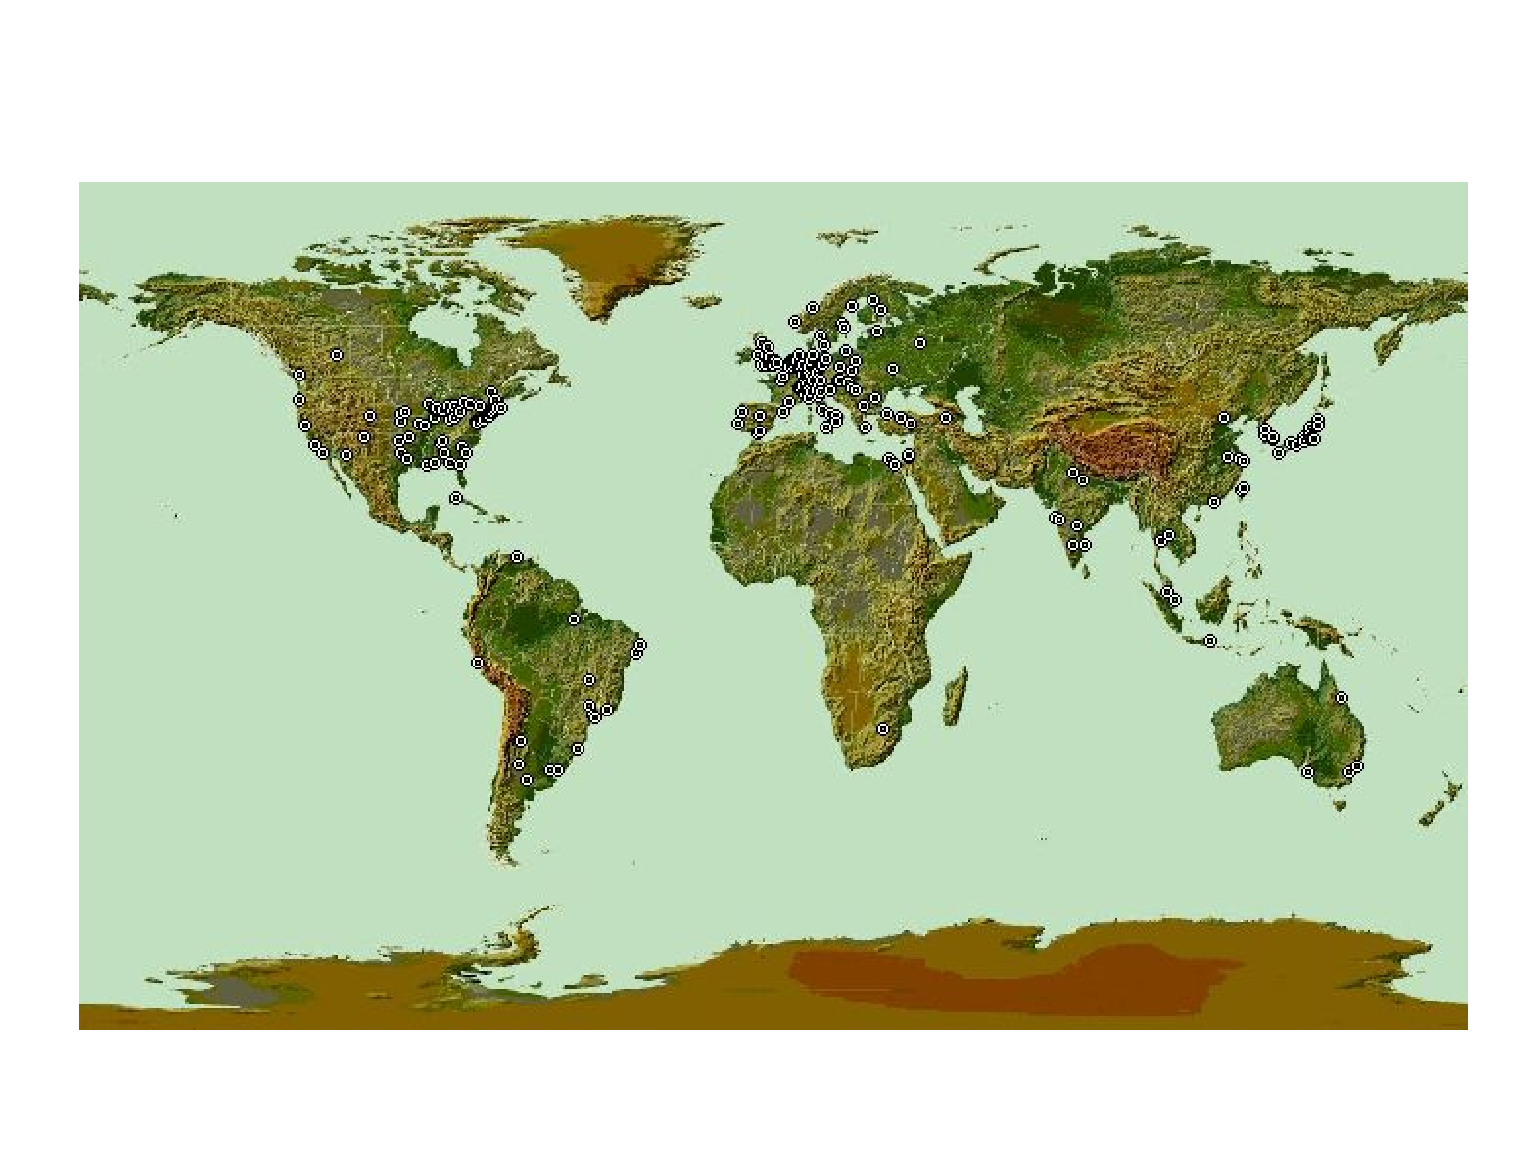
\includegraphics[width=\textwidth, height=!]
		    {figures/figure_1.eps}
  \end{center}
\end{figure}
\clearpage
\pagebreak[4] 

\begin{figure}[htbp]
  \begin{center}
    \caption[
      Illustration of the standard double-loop and the improved pairlist
      algorithm for a set of 10 atoms or charge groups. The standard
      algorithm scans the triangular atom-pair matrix row by row (top,
      unshaded box). A quadratic (top, light grey shade) or rhombic (top,
      dark grey shade) window scans more atom pairs for a given number of
      atoms loaded into processor cache. The triangular
      atom-pair matrix may be
      reordered to become rectangular (bottom), in which case the rhombic window
      becomes quadratic.
    ]{}
    \labfig{dirk}
    \includegraphics[width=\textwidth, height=!]
		    {figures/figure_2.eps}
  \end{center}
\end{figure}
\clearpage
\pagebreak[4] 


\begin{figure}[htbp]
  \begin{center}
    \caption[Interface of the {\tt Algorithm} class.]{}
    \labfig{gXX-algorithm}
    \vspace{0.7cm}
    \begin{lstlisting}[breaklines=true, caption={}, frame=, label=]
      class Algorithm{
	public:
	Algorithm(string name) : name(name) {}
	~Algorithm() {}
	virtual int init(Topology & topo,
	                 Configuration & conf,
			 Simulation & sim) = 0;

	virtual int apply(Topology & topo,
	                  Configuration & conf,
			  Simulation & sim) = 0;

	string name;
      };
    \end{lstlisting}
  \end{center}
\end{figure}
\clearpage
\pagebreak[4] 

\begin{figure}[htbp]
  \begin{center}
    \caption[Interface of the {\tt Algorithm\_Sequence} class.]{}
    \labfig{gXX-algorithmseq}
    \vspace{0.7cm}
    \begin{lstlisting}[breaklines=true, caption={}, frame=, label=]
      class Algorithm_Sequence : public vector<Algorithm *> {
	public:
	Algorithm_Sequence();
	~Algorithm();

	int init(Topology & topo,
	         Configuration & conf,
		 Simulation & sim);

	int run(Topology & topo,
	        Configuration & conf,
		Simulation & sim);

	Algorithm * algorithm(string name);
      };
    \end{lstlisting}
  \end{center}
\end{figure}
\clearpage
\pagebreak[4] 


\begin{figure}[ht]
  \begin{center}
    \caption[
      Illustration of the {\tt Interaction} classes in \noun{MD++}. The red
      arrows denote a {\em is-a} relationship, the black arrows {\em
	has-a}. All {\tt Interaction} classes inherit from {\tt Interaction}
      and, therefore, can be stored in the {\tt Forcefield}, which is a
      {\tt vector} of {\tt Interaction} classes. The {\tt
	Nonbonded\_Interaction} consists of a {\tt Pairlist\_Algorithm} (either
      a {\tt Standard\_Pairlist\_Algorithm} or a {\tt
	Grid\_Pairlist\_Algorithm}) and (depending on parallelisation) one or
      more {\tt Nonbonded\_Set}s. Those, in turn, consist of {\tt Storage}
      (to locally store forces, energies, virial tensor and pair lists) and
      an {\tt Outerloop} (to calculate the interactions). The {\tt Outerloop}
      relies on the {\tt Innerloop} and on {\tt Term} to calculate the
      interactions.
    ]{}
    \labfig{gXX-classes}
    \vspace{0.7cm}
    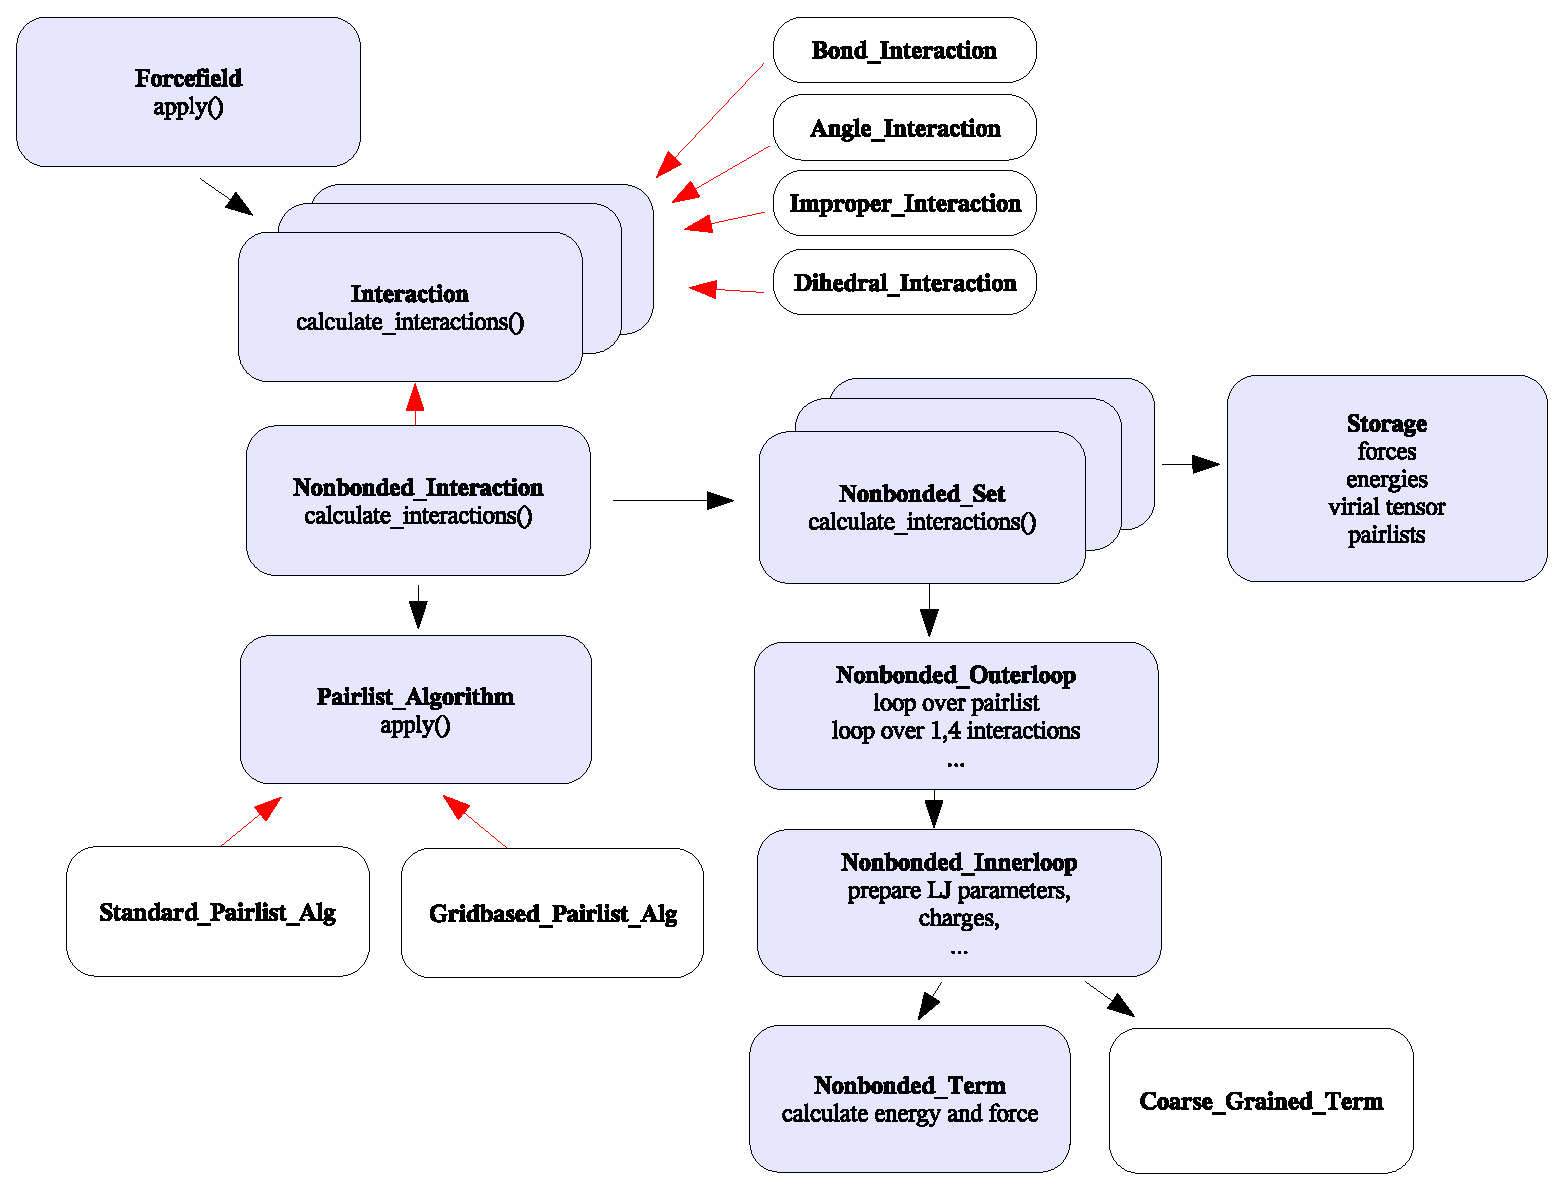
\includegraphics[width=\textwidth, height=!]
		    {figures/figure_5.eps}
  \end{center}
\end{figure}
\clearpage
\pagebreak[4] 

\begin{figure}[htbp]
%\doublespacing
\begin{center}
  \caption[Specialised code generation using templates.]{}
  \labfig{templates}
  \vspace{0.7cm}
  \begin{lstlisting}[breaklines=true, caption={}, frame=, label=]
  enum boundary_type {vacuum, rectangular, triclinic};
  template<boundary_type boundary>
  class Periodicity;
    
  template<>
  class Periodicity<vacuum>{
    public:
    void nearest_image(Vec const & v1, Vec const & v2,
                       Vec & v3);
  };

  template<>
  class Periodicity<rectangular>{
    public:
      void nearest_image(Vec const & v1, Vec const & v2,
                         Vec & v3);
  };

  template<>
  class Periodicity<triclinic>{
    public:
      void nearest_image(Vec const & v1, Vec const & v2,
                         Vec & v3);
  };

  template<boundary_type boundary>
  class Interaction{
    public:
      virtual int calculate_interactions(
        Topology const & topology,
	Configuration & configuration,
	Simulation const & simulation){

	  Vec v;
	  Periodicity<boundary>
	    periodicity(configuration.current().box);

	  periodicity.nearest_image(
	    configuration.current().pos(0),
	    configuration.current().pos(1),
	    v);

	  // and so on
        }
  };
\end{lstlisting}
\end{center}
\end{figure}
\clearpage
\pagebreak[4] 

\begin{figure}[htbp]
%\doublespacing
\begin{center}
\caption[Using the periodicity class.]{}
\labfig{templates2}
\vspace{0.7cm}
\begin{lstlisting}[breaklines=true, caption={}, frame=, label=]

  int main(int argc, char **argv){

    Interaction<triclinic> interaction;
    interaction.calculate_interactions(
      topology, configuration, simulation);
      
    return 0;
  }
\end{lstlisting}
\end{center}
\end{figure}
\clearpage
\pagebreak[4] 

\begin{figure}[ht]
  \begin{center}
    \caption[
      Glucose molecule with atom numbering
    ]{}
    \labfig{glucose}
    \includegraphics[width=\textwidth, height=!]
		    {figures/figure_8.eps}
  \end{center}
\end{figure}
\clearpage
\pagebreak[4] 

\begin{figure}[ht]
  \begin{center}
    \caption[
      Time course of the six torsional dihedral angles of the glucose ring
      as obtained from standard MD (A) and local-elevation (LE-) MD
      (B). The LE weight factor was $E_{\phi}^{le} = 2\,kJ\,mol^{-1}$ and
      the four torsional angles C(1)-C(2)-C(3)-C(4), C(2)-C(3)-C(4)-C(5),
      C(3)-C(4)-C(5)-O(5) and C(5)-O(5)-C(1)-C(2) were chosen as LE
      degrees of freedom.
    ]{}
    \labfig{glucose-LE}
    \vspace{2.0cm}
    \rotatebox[origin=c]{270}{
      \includegraphics[width=!, height=\textwidth]
		      {figures/figure_9.epsi}
    }
  \end{center}
\end{figure}
\clearpage
\pagebreak[4] 

\begin{figure}[ht]
  \begin{center}
    \caption[
      REMD of liquid butane, starting from an all {\em trans} configuration of
      the torsional angle.
      The path in $\lambda$ - space for the 11 replicas (starting at
      $\lambda$ values 0.0, 0.1, 0.2, 0.25, 0.3, 0.35, 0.4, 0.45, 0.5,
      0.55 and 0.6) is shown. Exchanges were attempted every 0.5 ps, in
      total 250. The overall exchange probability was 0.25.
    ]{}
    \labfig{re-lambda}
    \vspace{2.0cm}
    \rotatebox[c]{270}{
      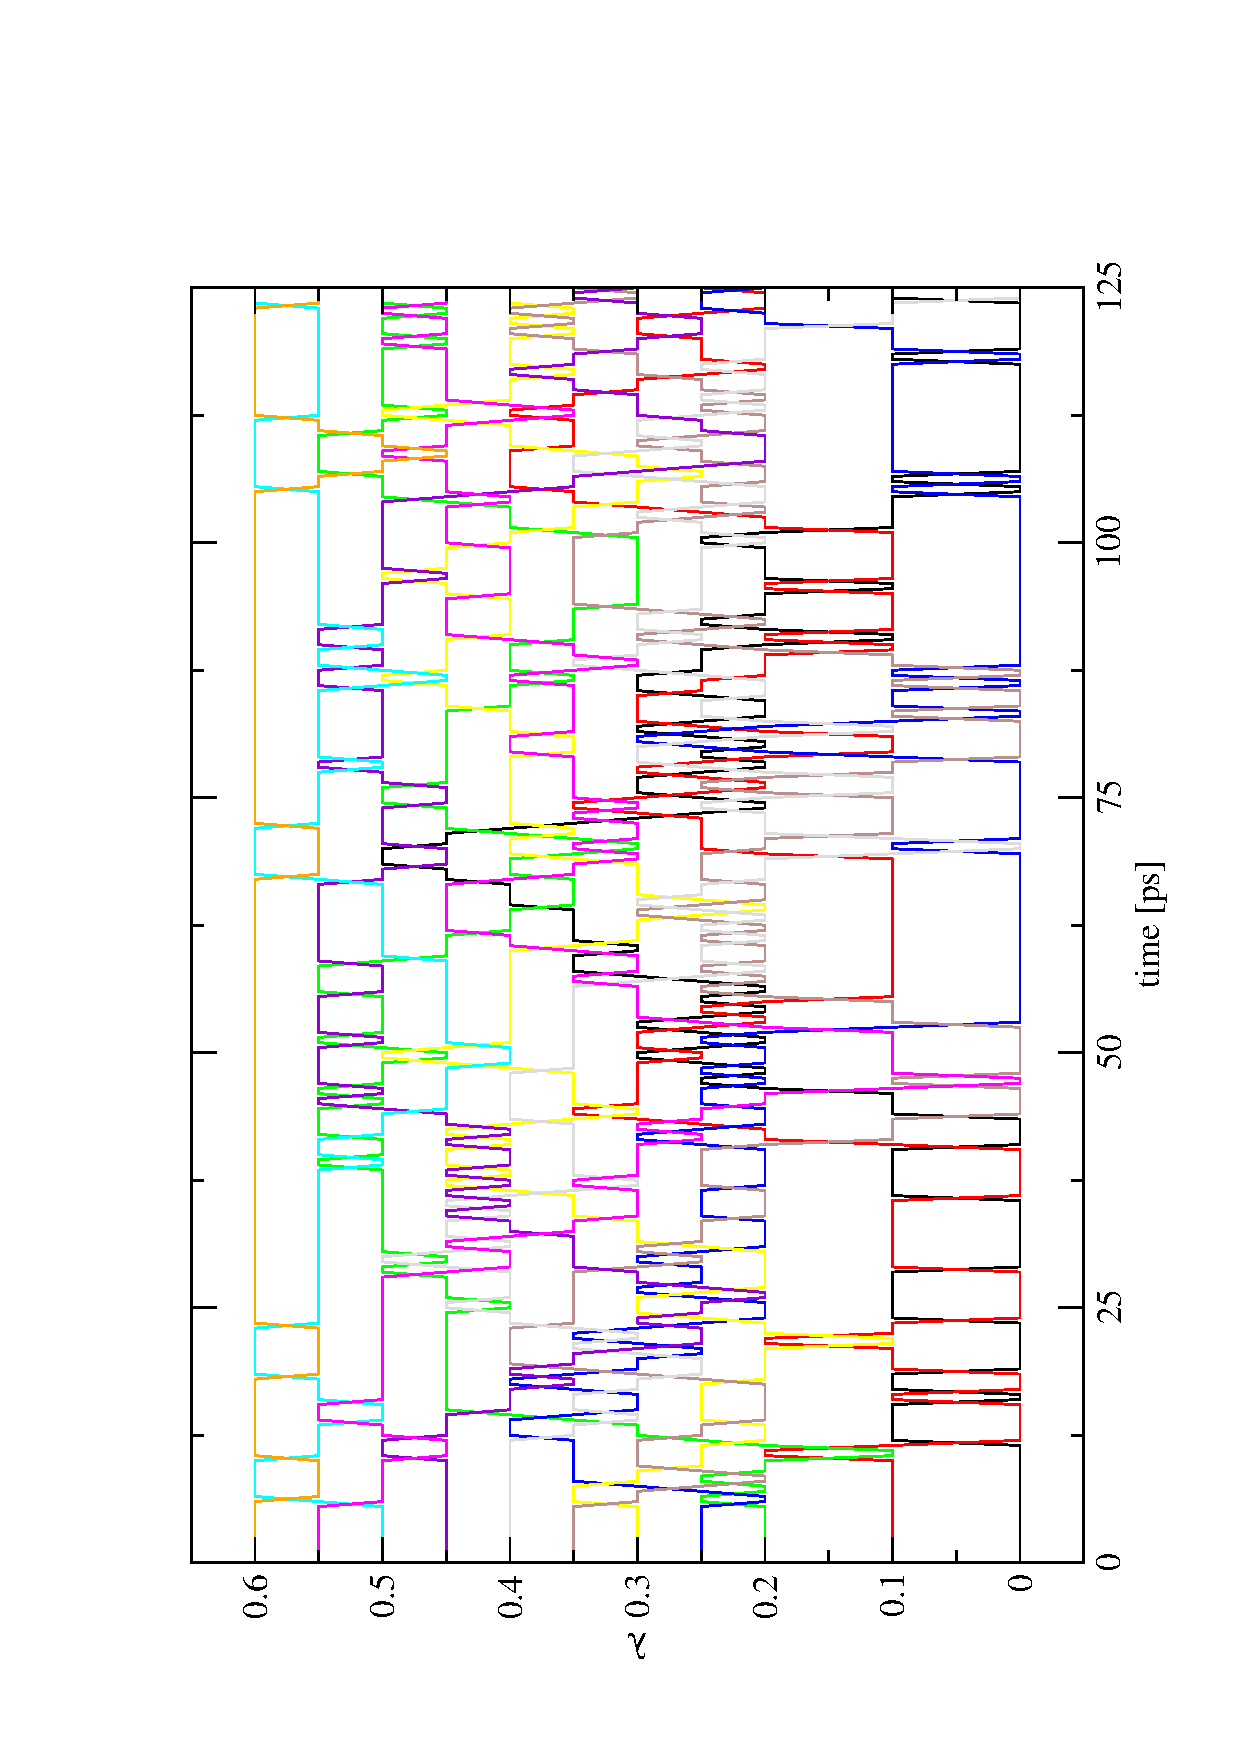
\includegraphics[width=!, height=\textwidth]
		      {figures/figure_10.epsi}
    }
  \end{center}
\end{figure}
\clearpage
\pagebreak[4] 

\begin{figure}[ht]
  \begin{center}
    \caption[
      Simulation of liquid butane, starting from an all {\em trans}
      configuration of the torsional angle. The time series of the
      root-mean-square deviation (rmsd) from the average torsional angle is
      shown. The bold black line depicts the rmsd in the standard MD
      simulation. No
      broadening of the distribution is visible. The bold red line
      denotes the rmsd of the replica at  $\lambda_i = 0.0$ (corresponding
      to the standard
      MD simulation). Clearly, the relaxation towards the equilibrium
      state is much faster using the replica-exchange method than in the
      standard MD simulation. The other
      lines denote the other replicas (at $0.0 < \lambda_i \le 1.0$, many
      of them reaching their
      equilibrium state already after about 50 ps.
    ]{}
    \labfig{re-rmsd}
    \vspace{2.0cm}
    \rotatebox[c]{270}{
      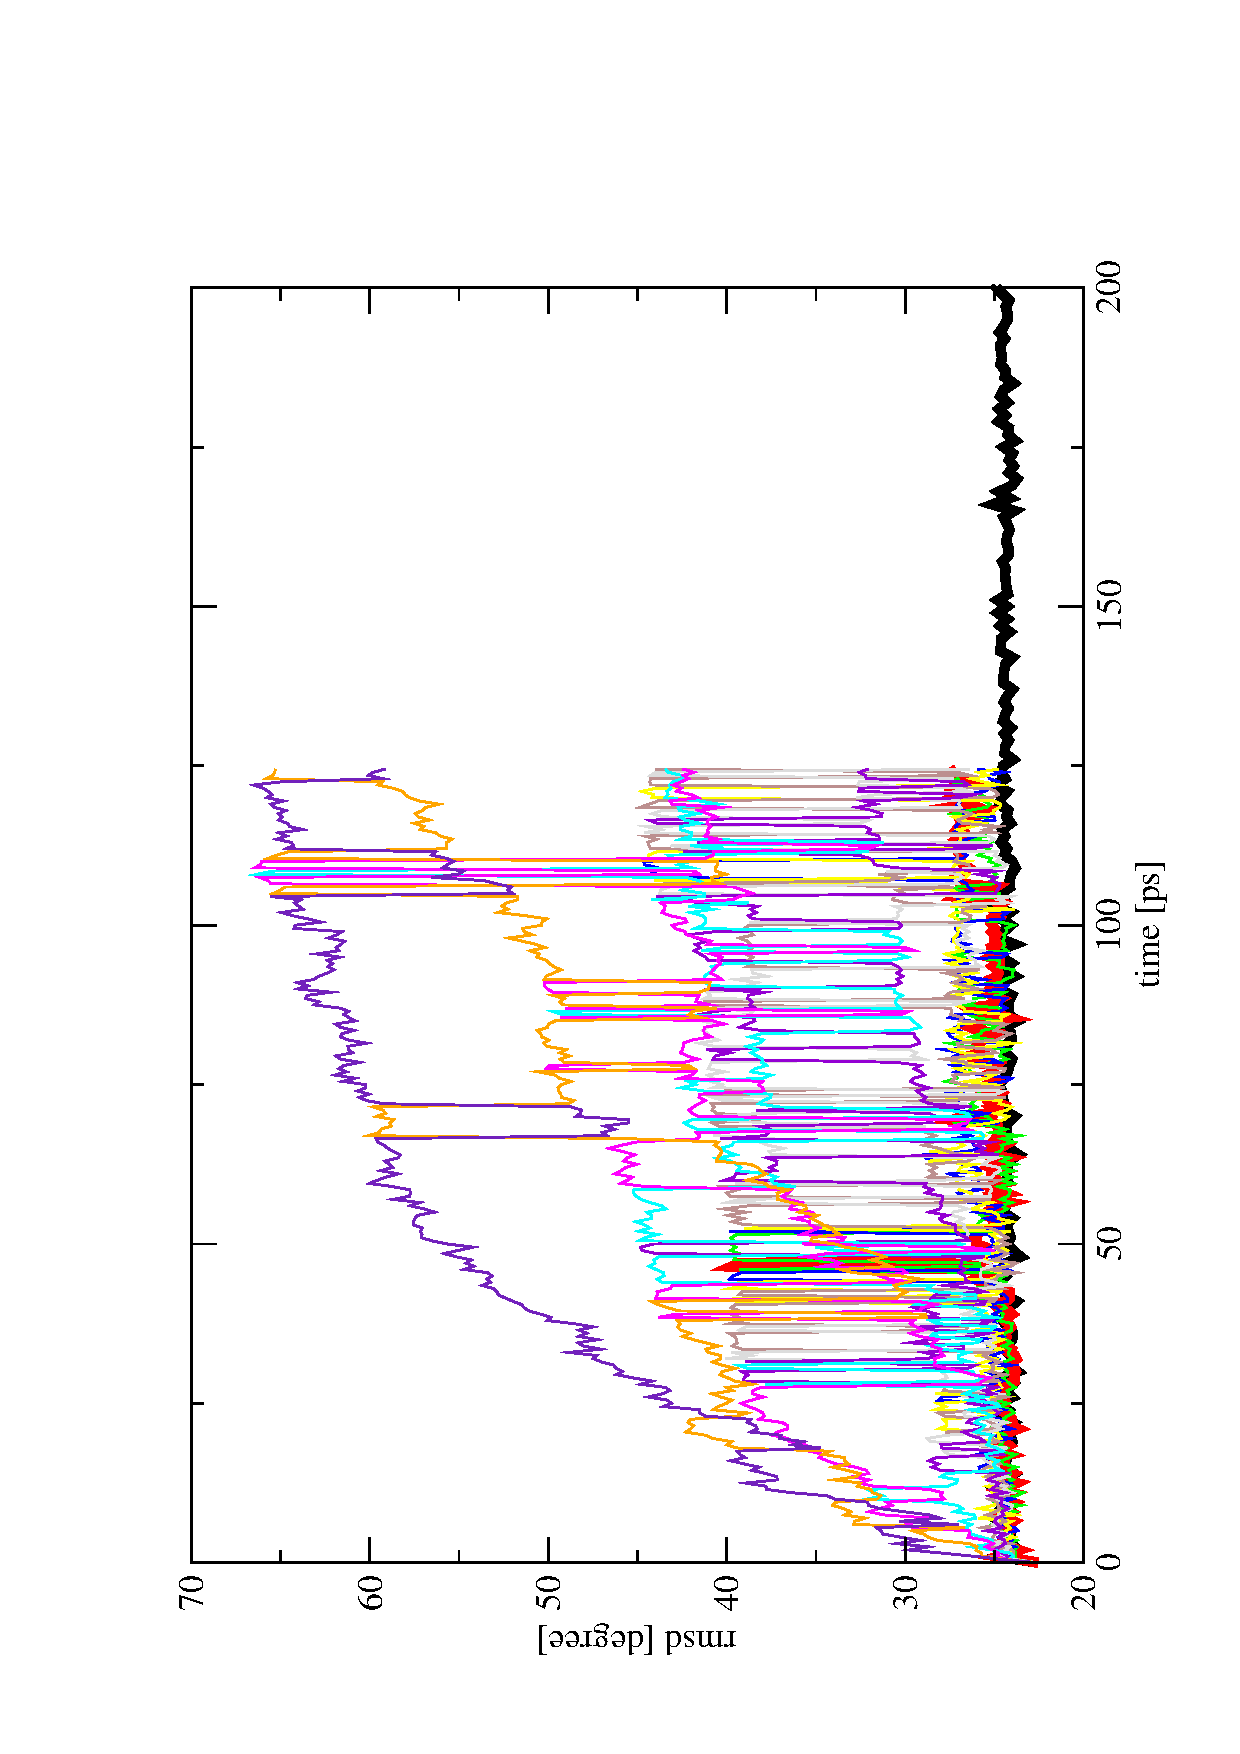
\includegraphics[width=!, height=\textwidth]
		      {figures/figure_11.epsi}
    }
  \end{center}
\end{figure}
\clearpage
\pagebreak[4] 

\begin{figure}[ht]
  \begin{center}
    \caption[
      Bond-angle (A-B-C, B-C-D) and torsional dihedral angle (A-B-C-D)
      distributions at the coarse-grained level. Grey: A-D are centres of
      mass of fragments consisting of four united atoms as obtained from
      AL trajectories. Black: A-D are beads of the CG model obtained from
      CG simulations.
    ]{}
    \labfig{cg-dist}
    \vspace{6.0cm}
    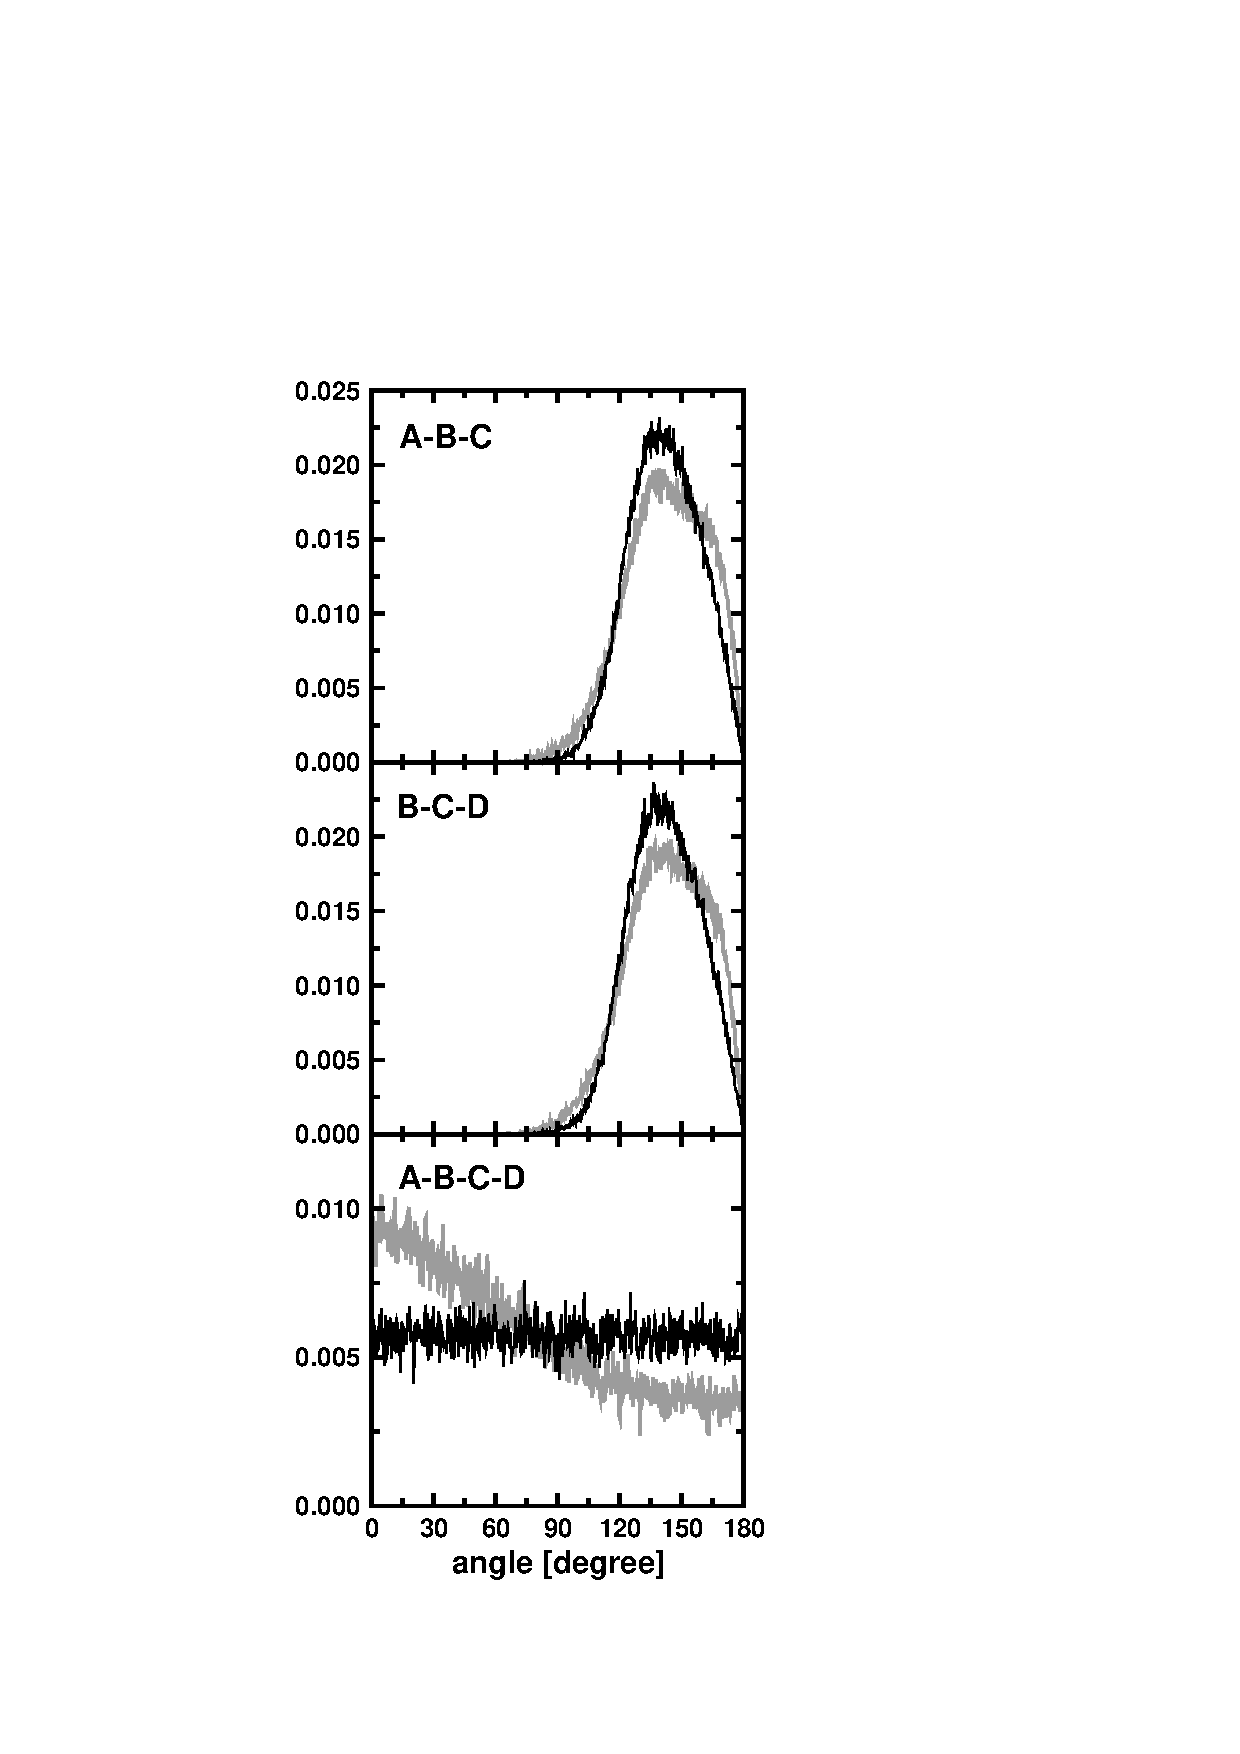
\includegraphics[width=7cm, height=!]
		    {figures/figure_12.epsi}
  \end{center}
\end{figure}
\clearpage
\pagebreak[4] 

\begin{figure}[ht]
  \begin{center}
    \caption[
      Polysubstituted byphenyls. Soft-core sites in the reference state
      are indicated as spheres. Of the $4 \cdot 2^9$ real ligands for
      which the relative free energy of binding to the estrogen receptor
      were calculated, the ones with lowest free energy of binding (in
      $kJ\,mol^{-1}$) are shown.
    ]{}
    \labfig{1step-biphenyl}
    \vspace{0.7cm}
    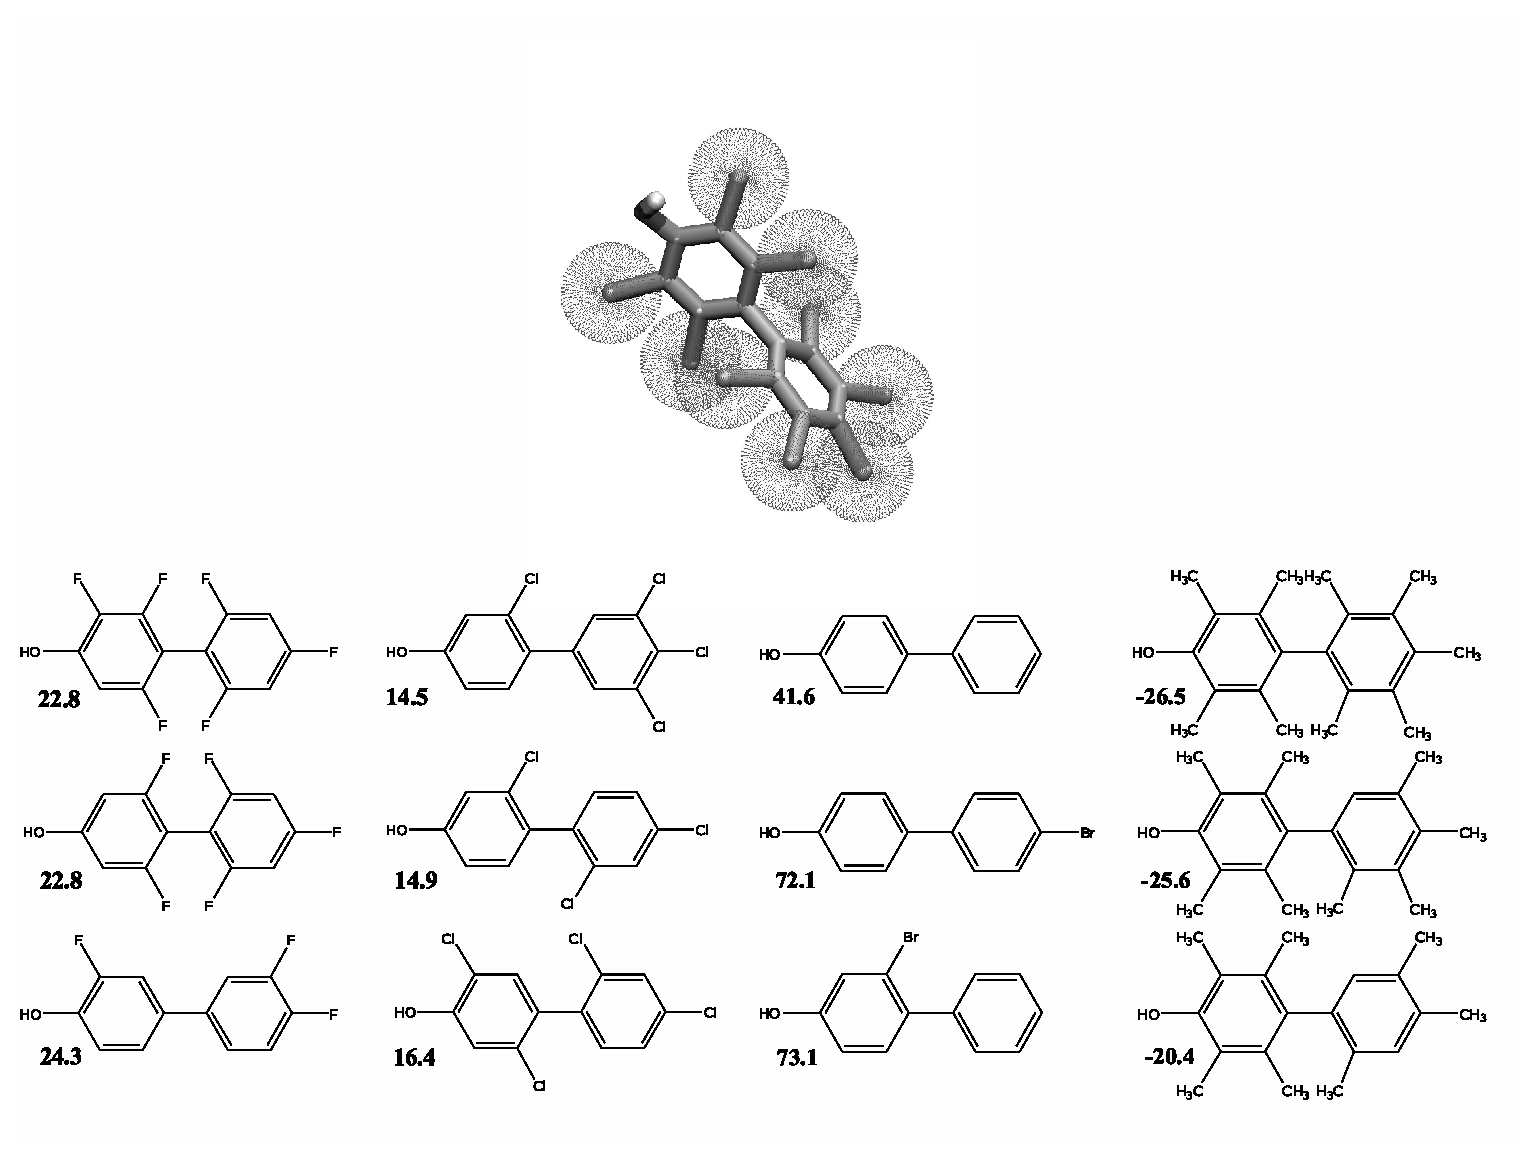
\includegraphics[width=\textwidth, height=!]
		    {figures/figure_13.eps}
  \end{center}
\end{figure}


\clearpage
\pagebreak[4] 

\clearpage
\end{document}
